\documentclass[11pt]{article}
\usepackage[margin=1in]{geometry}
\usepackage{amsmath,booktabs,array,longtable,fontspec,unicode-math,graphicx,xcolor,pgfplots}
\setmainfont{texgyrepagella-regular.otf}[BoldFont=texgyrepagella-bold.otf,ItalicFont=texgyrepagella-italic.otf]
\setmathfont{latinmodern-math.otf}
\usepackage[colorlinks=true,linkcolor=blue,citecolor=blue,urlcolor=blue]{hyperref}
\pgfplotsset{compat=1.18}
\emergencystretch=3em
\newtheorem{theorem}{Theorem}[section]
\newtheorem{proposition}[theorem]{Proposition}
\newtheorem{lemma}[theorem]{Lemma}
\newtheorem{corollary}[theorem]{Corollary}
\newenvironment{proof}{\par\noindent\textit{Proof.}\ }{\hfill$\mdlgwhtsquare$\par\medskip}
\newcommand{\E}{\mathbb E}
\newcommand{\R}{\mathbb R}
\newcommand{\Prob}{\mathbb P}
\newcommand{\Var}{\operatorname{Var}}
\newcommand{\Cov}{\operatorname{Cov}}
\newcommand{\PCS}{\operatorname{PCS}}
\newcommand{\KL}{\operatorname{KL}}
\newcommand{\diag}{\operatorname{diag}}
\newcommand{\argmax}{\operatorname*{arg\,max}}
\newcommand{\argmin}{\operatorname*{arg\,min}}
\newcommand{\one}{\mathbf1}
\newcommand{\pos}[1]{\left(#1\right)_+}
\title{Learning from Correlated and Persistent Web Rewards:\\Graph Alignment, General Autoregressive Bandits,\\Prediction, Regret, and Correct Selection}
\author{Extended working manuscript}
\date{9 October 2026}
\begin{document}
\maketitle
\begin{abstract}
Web alternatives share both long-run structure and persistent fluctuations. We collect a research program on sequential decisions with fixed unknown means, graph restrictions on their differences, and heterogeneous autoregressive deviations driven by spatially correlated innovations. The two graph roles are distinct: a covariance of transient shocks does not certify similar permanent means. We develop graph-regularized likelihood estimation, adaptive innovation regression, simultaneous confidence, correct stopping, and objective-specific UCB and correlated Gaussian sampling policies. A conservative certified-UCB bound gives sublinear stationary mean pseudo-regret under known stable dynamics; regret against an oracle observing every current state has an irreducible linear innovation term. Graph-energy information design distinguishes normalized paths from cliques even when their resistance diameters agree. Exact short-horizon control and Gaussian selection calculations clarify why sampling for immediate reward differs from sampling for final identification. We synthesize fixed-truth 100-arm AR(20) simulations, smaller general-AR schedule experiments, an alternative Bayesian toy, and KuaiRec graph and daily-engagement studies. A new laptop-sized Wikipedia experiment uses two fixed 24-article panels, pre-2024 hyperlink graphs, 2024 fitting, and selectively observed 2025 attention.
The application comparisons show budget-dependent gains from joint filtering, strong static baselines with mature history, and little measurable advantage of real hyperlink topology over degree-preserving rewiring.

Full derivations and source evidence accompany this deliberately uncompressed manuscript. Known-parameter guarantees, fitted-model heuristics, and exploratory application evidence are stated separately.
\end{abstract}
\clearpage
\tableofcontents
\clearpage
\section{A common question across Web learning and ranking-and-selection}

An item can be attractive because its permanent quality is high, because a persistent event temporarily raises demand, or because a shared platform shock affects many items. A measurement mixes these effects. Its usefulness depends on the decision: earning reward now, predicting a later reward, learning the best long-run alternative, or making a correct final selection. A graph can constrain permanent differences, correlate innovation noise, or do both. Treating these mechanisms as interchangeable obscures both the regret comparator and the information in a reading.

On the Web, navigation and co-engagement graphs arise naturally, while observations of detailed engagement or downstream opportunities can be selectively available. Our application interpretation is budgeted attention monitoring and opportunity selection. Recorded attention is an exogenous utility proxy; it does not measure the incremental engagement caused by displaying or promoting an item. This distinction is essential when interpreting offline panels.

The research began with similarity-based ranking and selection and developed along two streams. The graph stream asks how a supplied restriction eliminates statistically difficult alternatives and when graph construction is accurate enough to justify pooling. The temporal stream asks how sampling loses or preserves predictive information when unobserved arms continue evolving. Their combination retains fixed unknown means and a joint spatial innovation distribution, while allowing general, heterogeneous AR orders.

This document is a full research manuscript and evidence collection for later reduction. It includes the current mathematical results, algorithm definitions, experiments, negative findings, and application limitations. Appendices preserve complete technical derivations rather than omitting them for a conference page limit. An evidence manifest fingerprints the source versions used in the collection.

\subsection{Results and assumptions at a glance}
\begin{center}\small
\begin{tabular}{>{\raggedright\arraybackslash}p{.25\textwidth}>{\raggedright\arraybackslash}p{.32\textwidth}>{\raggedright\arraybackslash}p{.33\textwidth}}
\toprule
Result & What is established & Main condition \\
\midrule
Joint innovation likelihood & Exact predictable experiments and adaptive mean information & Known stable AR parameters, correct covariance/noise \\
Mean confidence and stopping & All-time contrast bounds and correct stopped recommendation & Fixed graph, supplied norm/energy bounds \\
Mean-UCB regret & Conservative sublinear mean pseudo-regret & Same assumptions, coverage probes \\
Current-state oracle floor & Positive expected linear innovation coefficient & Stationary Gaussian model, nondegenerate innovation contrasts \\
Graph information geometry & General design, resistance sensitivity, path--clique separation & Trusted graph-energy class; iid Gaussian information calculation \\
Selection formulas & Exact fixed-design Gaussian PCS and special allocation optima & Specific clock, prior, gap and observation conditions \\
Practical sampling & Mean, state, predictable-state and contrast rules & UCB/TS variants without a general optimality claim \\
Web data & Temporal modelling and topology controls on KuaiRec and Wikipedia & Exploratory selective-observation emulation \\
\bottomrule
\end{tabular}\end{center}

The current guarantees do not establish optimal restless control, sharp general graph-dependent temporal constants, learned-parameter confidence, or a universally best policy. These are meaningful future questions, rather than conditions silently assumed satisfied by the applications.

\section{Relation to existing theory}

Classical bounded stationary stochastic bandits have minimax regret of order $\sqrt{NT}$ for $T\ge N$, and important families have algorithms matching fixed-instance asymptotic information lower bounds~\cite{collected20,collected21,collected22}. A useful dependency model therefore restricts the alternatives the learner must distinguish, changes the information per observation, or changes the objective. It does not improve an unrestricted classical problem merely by smoothing estimates.

Spectral bandits and graph pure exploration already use graph-smooth reward means~\cite{collected1,collected17,collected2}. Clustered bandits already connect width and separation to regret~\cite{collected18,collected19}. Structured-bandit information programs and effective-resistance experimental design are established tools~\cite{collected11,collected24}. Our graph stream specializes them to quantitative energy restrictions, graph geometry and cumulative decisions. Its candidate incremental contribution is the explicit information sensitivity and a geometry-dependent achieved separation, not the general idea that similar arms share information. The original spectral selection index and its Operations Research follow-up motivate this question in ranking-and-selection~\cite{collected14,collected15,collected16}.

Time-varying Gaussian-process bandits already combine spatial and temporal kernels~\cite{collected3}. Shared linear-Gaussian and latent-AR bandits already use one action to learn about other actions and future rewards~\cite{collected4,collected5}. Predictive Sampling studies the remaining lifetime of information~\cite{collected10}; knowledge gradient studies the value of information for later decisions~\cite{collected6,collected30}. General AR processes become linear state-space models after stacking lags. Consequently, the joint filter itself is established machinery~\cite{collected33}. Our synthesis emphasizes the distinction between deterministic permanent-mean structure and correlated transient noise, adaptive likelihood under general orders, and sampling rules matched to different objectives.

Feedback graphs are a different observation model: they reveal neighbours' outcomes after a pull. Here an edge supplies a statistical restriction or covariance, and a pull directly reveals only selected coordinates. Neither the graph nor the filter manufactures additional observations. Full publication priority for each specialization remains unestablished; the original novelty audit is preserved in the evidence directory.

\section{Fixed means, restless rewards and two graph roles}

There are $N$ arms with deterministic unknown means $\mu_i$. Before observing the current field, select $a_t$ and receive
\begin{equation}
X_{i,t}=\mu_i+z_{i,t},\qquad
z_{i,t}=\sum_{r=1}^{p_i}a_{i,r}z_{i,t-r}+\eta_{i,t},\qquad
Y_t=X_{a_t,t}+\xi_t.
\label{eq:mainmodel}
\end{equation}
The innovations satisfy $\eta_t\stackrel{\mathrm{iid}}\sim N(0,Q_\eta)$, $Q_\eta\succ0$, while independent observation noise has variance $r\ge0$. AR polynomials are stable. All arms evolve every calendar time, whether sampled or not. For the theoretical results, orders, coefficients, innovation covariance, observation noise and stationary initialization are known.

Put $c_i=1-\sum_ra_{i,r}$. The raw AR intercept is $c_i\mu_i$, not $\mu_i$. Means are not regenerated between repeated-noise experiments. Algorithmic Gaussian draws represent uncertainty at a fixed truth. Some older special-case results explicitly average over a Gaussian prior; they are separately marked in the appendices.

Let $L_\mu$ be a candidate mean Laplacian and impose, when justified,
\begin{equation}
\mu^\top L_\mu\mu\le S^2,\qquad \|\mu\|_2\le B.
\end{equation}
This is deterministic side information. Independently, an innovation graph can supply a covariance such as a rescaled inverse of $\alpha_\eta I+\lambda_\eta L_\eta$. One graph may serve both roles, but that is an additional substantive assumption. Shared noise alone cannot identify the mean of an arm that never appears in the measurement design: the likelihood has no column for that mean. Mean regularization needs its own justification.

\subsection{The full lag process}
Stack lag deviations into $s_t$ and write
\begin{equation}
s_{t+1}=Fs_t+E\eta_{t+1},\qquad z_t=Cs_t,\qquad
\Gamma=F\Gamma F^\top+EQ_\eta E^\top.
\end{equation}
The stationary node-time covariance is
\begin{equation}
G_h=CF^h\Gamma C^\top,\qquad
(G_h)_{ij}=(Q_\eta)_{ij}\sum_{k\ge0}\psi_i(k+h)\psi_j(k),\quad h\ge0,
\end{equation}
where $\psi_i$ is the impulse-response sequence. Reverse-time covariances are transposes. Heterogeneous AR filters generally make $G_h$ asymmetric for positive lags and prevent a separable spatial-times-temporal kernel. A lag-20 process can have no one-period correlation but substantial dependence twenty periods later.

\subsection{Comparators must be fixed before designing a policy}
Let $b^*=\argmax_i\mu_i$. Four regrets are distinct:
\begin{align}
R_{\rm current}(T)&=\sum_t[\max_iX_{i,t}-X_{a_t,t}],\\
R_\mu(T)&=\sum_t[\mu_{b^*}-\mu_{a_t}],\\
R_{\rm stationary}(T)&=T\mu_{b^*}-\sum_tX_{a_t,t},\\
R_{\rm fixed}(T)&=\sum_t[X_{b^*,t}-X_{a_t,t}].
\end{align}
The first two are nonnegative pathwise. The latter two may be negative because adaptive decisions exploit predictable positive deviations. Under stationary initialization,
\begin{equation}
\E R_{\rm stationary}=\E R_{\rm fixed}
=\E R_\mu-\sum_t\E z_{a_t,t}.
\end{equation}
Terminal PCS is $\Pr(\widehat b_T=b^*)$ over repeated noise at a fixed truth. It is not the probability of finding the largest last reward. Pure exploration can spend reward to resolve a difficult permanent contrast, while a tracking policy can earn high actual reward from an arm with a lower permanent mean.

\section{Graph estimation using the correct trajectory likelihood}

For a fixed sampling schedule, let $M$ select the observed coordinates and $\Xi$ be their joint AR covariance including measurement noise. Then $Y\sim N(M\mu,\Xi)$ and
\begin{equation}
\mathcal I=M^\top\Xi^{-1}M,\quad q=M^\top\Xi^{-1}Y,\quad
\widehat\mu_H=(\mathcal I+H)^{-1}q,\qquad H=\alpha I+\lambda L_\mu.
\end{equation}
Spatial smoothness enters estimation through $H$; the graph-correlated AR likelihood enters through $\Xi$. Ignoring either changes the inference problem.

For a deterministic design and penalty, with $J=\mathcal I+H$,
\begin{equation}
\E\widehat\mu_H-\mu=-J^{-1}H\mu,\qquad
\Var(\widehat\mu_H)=J^{-1}\mathcal I J^{-1}.
\end{equation}
Inverse penalized information is not the repeated-noise covariance of a biased estimator. With $H=\lambda L_\mu$, the graph-energy bias of contrast $v$ is bounded by
\begin{equation}
\lambda S\sqrt{v^\top J^{-1}L_\mu J^{-1}v}.
\end{equation}
The common offset is unpenalized by a Laplacian. A proper $\alpha I$ regularizer is used for adaptive confidence.

An energy-constrained estimator literally imposes $\nu^\top L_\mu\nu\le S^2$. If its constraint is active, KKT gives
\begin{equation}
\widehat\mu_S=(\mathcal I+\lambda_*L_\mu)^{-1}q,
\qquad \widehat\mu_S^\top L_\mu\widehat\mu_S=S^2.
\end{equation}
Energy decreases monotonically along the positive multiplier, allowing a scalar search. Enforcing an estimate's radius does not establish that the unknown truth satisfies that radius. Same-data tuning of the graph or multiplier needs an uncertainty argument beyond fixed-penalty Gaussian calculations.

\subsection{Adaptive actions require predictable innovations}
Before time $t$, conditional on a candidate fixed $\mu$, maintain
$s_t\mid\mu,\mathcal H_t\sim N(g_t+D_t\mu,P_t)$. With $\ell_a=C^\top e_a$, define
\begin{equation}
v_{t,a}=e_a+D_t^\top\ell_a,\qquad d_{t,a}=\ell_a^\top P_t\ell_a+r,\qquad u_{t,a}=v_{t,a}/\sqrt{d_{t,a}}.
\end{equation}
The selected normalized observation is exactly
\begin{equation}
R_t=\frac{Y_t-\ell_{a_t}^\top g_t}{\sqrt{d_{t,a_t}}}
=u_t^\top\mu+\epsilon_t,\qquad \epsilon_t\mid\mathcal H_t,a_t\sim N(0,1).
\label{eq:maininnovation}
\end{equation}
Gaussian conditioning updates the affine mean and covariance, and propagation uses $F$. The designs $u_t$ are predictable even under adaptive actions. Thus
$\mathcal I_T=\sum_tu_tu_t^\top$ and $q_T=\sum_tu_tR_t$ match the recorded-path dense likelihood. This is an algebraic equality; it does not make an adaptively selected schedule an independent fixed design.

\section{Confidence, stopping, and stationary mean regret}

\begin{theorem}[Fixed-mean all-time contrast confidence]
Assume the correct known model, a graph fixed before measurement, $\mu^\top L_\mu\mu\le S^2$, $\|\mu\|\le B$, and $H=\alpha I+\lambda L_\mu\succ0$. With $J_T=H+\mathcal I_T$ and
\begin{equation}
\beta_T=\sqrt{\log\frac{\det J_T}{\det H}+2\log(1/\delta)}
+\sqrt{\alpha B^2+\lambda S^2},
\end{equation}
with probability at least $1-\delta$, simultaneously for all times and contrasts,
\begin{equation}
|v^\top(\widehat\mu_T-\mu)|\le\beta_T\sqrt{v^\top J_T^{-1}v}.
\end{equation}
\end{theorem}
\begin{proof}
The Gaussian innovation score $W_T=\sum_tu_t\epsilon_t$ admits the exponential martingale for every fixed vector. Mixing it with $N(0,H^{-1})$ yields
$\sqrt{\det H/\det J_T}\exp(\|W_T\|_{J_T^{-1}}^2/2)$. A crossing bound supplies the log-determinant term. The regularization contribution in $\widehat\mu_T-\mu=J_T^{-1}(W_T-H\mu)$ is bounded by $\sqrt{\mu^\top H\mu}$. Contrast Cauchy--Schwarz completes the result. The Gaussian mixing variable is a proof device, not a prior on the physical means.
\end{proof}

Stop and recommend $b=\argmax_i\widehat\mu_i$ only when every comparison exceeds its contrast width. The probability of an incorrect stopped recommendation is then at most $\delta$. A forced budget-terminal recommendation without passing the certificate has no such guarantee.

Let $A_i(e^{-\mathrm i\omega})$ be the AR polynomial on the unit circle and define
$a_{\min}=\min_{i,\omega}|A_i|$, $a_{\max}=\max_{i,\omega}|A_i|$. Put
\begin{equation}
v_-={\lambda_{\min}(Q_\eta)}/{a_{\max}^2}+r,
\qquad v_+={\lambda_{\max}(Q_\eta)}/{a_{\min}^2}+r.
\end{equation}
For every recorded schedule,
\begin{equation}
v_+^{-1}\diag(N_i(T))\preceq\mathcal I_T\preceq v_-^{-1}\diag(N_i(T)).
\end{equation}
These conservative spectral bounds permit consistency with growing coverage.

\begin{theorem}[Conservative certified mean-UCB bound]
After one initial reading of each arm, force cyclic probes at square calendar ages, with total forced count $F_T\le N+\sqrt T$. On other rounds select the largest $\widehat\mu_i+\beta\sqrt{(J^{-1})_{ii}}$. On the simultaneous event,
\begin{equation}
R_\mu(T)\le2BF_T+4\beta_T\sqrt{v_+NT},
\qquad
\beta_T\le\sqrt{N\log(1+T/(\alpha v_-))+2\log(1/\delta)}
+\sqrt{\alpha B^2+\lambda S^2}.
\end{equation}
For fixed dimensions and stable parameters this is sublinear.
\end{theorem}
\begin{proof}
Optimism bounds an ordinary action gap by twice its mean width. After initial coverage, $(J^{-1})_{ii}\le v_+/N_i$. Summing inverse square-root counts bounds ordinary regret by $4\beta_T\sqrt{v_+NT}$. Forced gaps are at most $2B$. The information upper bound and $H\succeq\alpha I$ bound the determinant.
\end{proof}
The expectation adds $2BT\delta$. A horizon-specific choice $\delta=1/T$ bounds that remainder. The experiment's practical UCB coefficient differs from the certified coefficient; a theorem for the latter must not be assigned to the former. This guarantee is conservative and does not give the sharp spatial or temporal regret coefficient.

\section{Graph alignment changes the alternative class}

Graph correctness has a quantitative meaning: a supplied restriction on means is actually true. Graph usefulness depends on the difficult alternatives that remain. Ordinal agreement or a lower smoothness quotient does not imply safe smoothing or a smaller regret constant for every policy.

Effective resistance gives
$|\mu_i-\mu_j|\le S\sqrt{(e_i-e_j)^\top L^\dagger(e_i-e_j)}$. This converts an energy radius into a component width. Certified pooling can then reject an entire suboptimal component when its uncertainty and supplied width are below its gap. Incorrectly small widths can remove the best arm and cause linear regret. Enlarging a valid certificate is safe but can remove most of the benefit.

\subsection{An exact graph-energy information design}
Consider a homogeneous suboptimal component of $m$ arms, gap $\Delta_c$, iid Gaussian observation variance $\sigma^2$, and supplied energy radius $S$. Let $s=S/\Delta_c$ and
\begin{equation}
F_L(p,s)=\min_i\min_{\substack{z\in[0,1]^m,\ z_i=1\\z^\top Lz\le s^2}}\sum_jp_jz_j^2,
\qquad F_L^*(s)=\max_{p\in\Delta_m}F_L(p,s).
\end{equation}
The structured information program gives component constant
\begin{equation}
C_{L,S}=\frac{2\sigma^2}{\Delta_cF_L^*(S/\Delta_c)}.
\end{equation}
For a fixed graph, $F_L^*$ decreases as the supplied uncertainty expands, lies in $[1/m,1]$, and equals one at zero energy. A finite-strength resolvent $(\diag(p)+\tau L)^{-1}$ solves the inner quadratic optimization. This connects the original spectral index with an information calculation; it is not itself a regret theorem for choosing the largest smoothed value.

Define the resistance radius
\begin{equation}
\rho_L=\min_{p\in\Delta_m}\max_i\sqrt{(e_i-p)^\top L^\dagger(e_i-p)}.
\end{equation}
It equals the radius of the minimum enclosing ball in the effective-resistance embedding, an established geometric object. Its local information sensitivity is
\begin{equation}
\frac{C_{L,S}}{2\sigma^2/\Delta_c}
=1+2(S/\Delta_c)\rho_L+O((S/\Delta_c)^2D),
\end{equation}
where $D$ is the resistance diameter. The radius, rather than diameter alone, sets the first-order price of the supplied uncertainty.

\subsection{A path--clique separation and an achieved policy result}
A clique with edge weight $1/m$ and a path with weight $(m-1)/2$ have resistance diameter two. At $S=\Delta_c$, every clique coordinate can independently become optimal, giving $C_{\rm clique}=2\sigma^2m/\Delta_c$. A half-and-half endpoint design on the path gives
\begin{equation}
C_{\rm path}\le\frac{2\sigma^2}{\Delta_c(1-1/\sqrt2)^2},
\end{equation}
which has no factor $m$. Identical component diameters therefore conceal a growing information separation.

Graph-design elimination with UCB fallback uses a preselected resistance design, valid energy allowances, capped stages and ordinary-arm fallback. Its proved finite-time result protects the optimal component and attains logarithmic regret without linear component-size dependence on the normalized path. It is not proved to match the exact information constant on general positive-uncertainty classes. Small-instance pilot overhead can make it substantially worse than ordinary UCB.

Certified Laplacian error also has an explicit price. If $(1-\zeta)L\preceq\widehat L\preceq(1+\zeta)L$, a radius $S$ under $L$ is safely enlarged to $\sqrt{1+\zeta}S$ under $\widehat L$. This repairs the mean restriction when the likelihood remains correct. It cannot repair a covariance likelihood fitted from the wrong graph.

\section{Combining pooling with persistent observations}

An innovation-regression confidence set permits certified component bounds even when observations are correlated over space and time. For a component $C$, a supplied diameter $\varepsilon_C$, estimate $m$, inverse information $V$, and confidence coefficient $\beta$, define
\begin{equation}
U_i=m_i+\beta\sqrt{V_{ii}},\qquad
U_C=\min\left\{\max_{i\in C}U_i,
\min_{w\in\Delta(C)}(w^\top m+\beta\sqrt{w^\top Vw})+\varepsilon_C\right\}.
\end{equation}
On the all-contrast event, both terms upper-bound the largest permanent mean in $C$. A selected suboptimal component with gap $\Delta_C>\varepsilon_C$ must satisfy
\begin{equation}
\min_{w\in\Delta(C)}w^\top Vw
\ge\frac{(\Delta_C-\varepsilon_C)^2}{4\beta^2}.
\end{equation}
This is a valid realized-information rejection condition. Converting it into a count-based regret formula needs an information-growth condition for the actual schedule. The spatially correlated case does not inherit an arbitrary per-pull constant from a full-field experiment.

\subsection{Two corrections needed when reusing the bridge notes}
The collected bridge notes contain proposed extensions, not a blanket new theorem. First, with independent-arm AR(1), one pull adds at least $(1-\phi)^2/(V+r)$ information to that arm under the stated positive-persistence filter conditions. The inverse variance of a pooled component depends on the \emph{sum} of arm information. Its per-pull increase has this same lower bound, not $|C|$ times that bound. A component-size factor requires $|C|$ scalar readings and must be charged accordingly.

Second, a simultaneous observation of a subset $S$ has innovation covariance $Q_{SS}$ and precision $(Q_{SS})^{-1}$. It does not generally have precision $(Q^{-1})_{SS}$: the latter conditions on the unobserved contemporaneous coordinates. For common coefficients and a continuously observed subset, the long-run comparison covariance is $Q_{SS}/c^2$, giving pair contrast variance $2q(1-\rho)/c^2$ in the equal-variance case. Arbitrary partial restless schedules need the exact conditional filter, rather than substitution of a full-field precision.

These corrections preserve the useful validity bridge while narrowing unverified information-growth claims. The main certified mean-UCB theorem does not rely on either incorrect factor.

\subsection{Persistence breaks iid confidence under bursty exposure}
For consecutive observations from stationary AR(1) with variance $V$,
\begin{equation}
\Var(\bar Y_n)=\frac Vn\left[\frac{1+\phi}{1-\phi}
-\frac{2\phi(1-\phi^n)}{n(1-\phi)^2}\right].
\end{equation}
An iid radius based on $V/n$ underestimates uncertainty. The limiting variance inflation is $(1+\phi)/(1-\phi)$. Widely separated UCB pulls may avoid much of this effect; bursty exposure reveals it. The coverage experiments report high iid miscoverage and erroneous irreversible elimination at strong persistence, whereas innovation-based certificates remain valid but can be so wide that they eliminate nothing. Correctness and the reward cost of that correctness must both be reported.

\section{Sampling rules for reward and permanent selection}

\subsection{Shared forecast and three uncertainty sources}
For past readings, define $K=\Cov(z_t,\text{selected past deviations})$, $A=K\Xi^{-1}$, $W=I-AM$, $V=(H+M^\top\Xi^{-1}M)^{-1}$ and $m=VM^\top\Xi^{-1}Y$. Then
\begin{equation}
f=AY+Wm,\qquad P=G_0-K\Xi^{-1}K^\top,\qquad \Sigma=P+WVW^\top.
\end{equation}
These working quantities distinguish uncertainty in fixed means, uncertainty about past lag states, and the current innovation. $\Sigma$ supports randomized decisions; frequentist confidence additionally includes regularization bias and adaptive uncertainty.

Mean UCB/TS acts on $m,V$. Full-state UCB/TS acts on $f,\Sigma$. Predictable-state UCB/TS acts on $f,\Sigma-Q_\eta$. The last matrix is positive semidefinite under the correct model because
\begin{equation}
z_t=CFs_{t-1}+\eta_t,
\qquad P-Q_\eta=\Var(CFs_{t-1}\mid\mathcal H_t,\mu)\succeq0.
\end{equation}
Removing fresh innovations retains learnable mean and past-state uncertainty. It can reduce futile randomized exploration. It remains a one-step heuristic and can undervalue delayed AR information. It is distinct from both future-information Predictive Sampling and the older KuaiRec mean-only perturbation rule.

All joint Gaussian perturbations preserve cross-arm covariance. Drawing independent arm marginals is an approximation and must be labelled. No standard linear-TS theorem is imported: the whitened design vector differs from the physical reward coordinate and changes with the history.

\subsection{Permanent-contrast allocation}
For contrast $v$ and a candidate normalized reading $u_{t,a}$, the exact reduction in inverse regularized information is
\begin{equation}
g_t(v,a)=\frac{(v^\top Vu_{t,a})^2}{1+u_{t,a}^\top Vu_{t,a}}
=\frac{(v^\top VW_{a,:}^\top)^2}{\Sigma_{aa}+r}.
\end{equation}
Contrast LUCB chooses a current best estimate and an optimistic challenger, then measures the arm maximizing this gain. Top-two Thompson contrast sampling draws plausible competing mean winners and uses the same gain. A third arm can best resolve their comparison. These are practical fixed-budget heuristics, not proved globally PCS-optimal allocations.

An observation's conditional reduction in a future target variance is
\begin{equation}
\Delta_{i,h}(a)=\frac{(e_i^\top CF^hP_t\ell_a)^2}{\ell_a^\top P_t\ell_a+r}.
\end{equation}
Replace $e_i$ by a contrast to value a future comparison. The entire impulse profile matters; one lag-one correlation coefficient is insufficient.

\subsection{What is the best policy in principle?}
With known parameters, the finite-horizon optimal policy solves the belief-state Bellman equation
\begin{equation}
J_h(b)=\max_a\{f_a(b)+\E[J_{h-1}(\mathcal T_a(b,Y_a))]\},\quad J_0=0.
\end{equation}
The state includes every mean and lag belief. Exactly two remaining decisions have a Gaussian knowledge-gradient score: immediate forecast plus the expected maximum of next forecasts after one observation. Independent arms admit a normal-density/CDF expression. In a joint graph state, one observation moves every next forecast, producing an expected maximum of correlated affine functions of one normal variable. Rolling that two-period score is feasible; it does not solve the general Bellman equation.

Long-horizon approximations can outperform Predictive Sampling at moderate persistence and lose at near-unit persistence. The optimality statements in the two-period and special selection theorems therefore do not imply a uniformly best indefinite-horizon sampling algorithm.

\section{Information limits and exact allocation cases}

\subsection{A linear floor against current-state information}
Let $\mathcal G(\mu,K)=\E\max_i(\mu_i+Z_i)$ for $Z\sim N(0,K)$. A genie seeing all past lag states and the true means has current conditional covariance $Q_\eta$. Its forecast field has covariance $G_0-Q_\eta$. Thus every causal policy's expected current-oracle regret satisfies
\begin{equation}
\E R_{\rm current}(T)\ge T\left[\mathcal G(\mu,G_0)-\mathcal G(\mu,G_0-Q_\eta)\right].
\end{equation}
Nondegenerate innovation contrasts make the coefficient positive. This is an expected floor, not a pathwise inequality, and generally not attainable with one selected reading per round. A known-mean greedy filter is a benchmark, not an optimal causal policy. For simultaneous $b$-arm sets replace the maximum by the sum of the largest $b$ coordinates and charge $bT$ measurements.

\subsection{Mean information and long-run covariance}
For noiseless full fields, with $p=\max_i p_i$ and $D_c=\diag(c_i)$,
\begin{equation}
\mathcal I_n=\mathcal I_p+(n-p)D_cQ_\eta^{-1}D_c,
\qquad \mathcal K_{\rm LR}=D_c^{-1}Q_\eta D_c^{-1}.
\end{equation}
Persistence can strengthen prediction while making permanent means harder to learn. In adaptive selected feedback,
\begin{equation}
\KL(P_\mu^{\pi,T},P_\nu^{\pi,T})
=\tfrac12\E_\mu[(\mu-\nu)^\top\mathcal I_T(\mu-\nu)].
\end{equation}
This identity yields comparison lower bounds by change of measure. It does not turn an arbitrary schedule into a consecutive full-field experiment.

\subsection{Two independent AR(1) means: exact schedules}
For exact stationary AR(1) observations separated by gaps $h_r$, variance $V$ and known $0\le\phi<1$,
\begin{equation}
I(\mathcal T_i)=\frac1V\left[1+\sum_{r=2}^{n_i}\frac{1-\phi^{h_r}}{1+\phi^{h_r}}\right].
\end{equation}
At fixed positive gap $\Delta$, fixed-schedule GLS comparison has PCS
$\Phi(\Delta/\sqrt{I_1^{-1}+I_2^{-1}})$. For even budget $T$, strict alternation is the optimal fixed calendar schedule, with per-arm information
\begin{equation}
I_*=\frac{T(1-\phi^2)+4\phi^2}{2V(1+\phi^2)}.
\end{equation}
Under the separate symmetric prior $\mu_i\sim N(0,\tau^2)$, alternation also attains the optimal prior-averaged adaptive PCS
$1/2+\arctan(\tau\sqrt{I_*})/\pi$. The prior-averaged theorem is not a uniform adaptive frequentist statement at every fixed pair.

For next-round terminal-state selection with known means, observing different arms in the last two rounds is adaptively optimal; older observations add no forecast information once exact latest states are known. The next-round PCS is
\begin{equation}
\frac12+\frac1\pi\arcsin\left(\phi\sqrt{(1+\phi^2)/2}\right).
\end{equation}
Changing the target to the last observed round changes the formula. This explains why large budgets can improve permanent identification without improving a particular terminal-state objective.

\subsection{General AR changes the allocation geometry}
For correlated lag-two processes $z_{i,t}=az_{i,t-2}+\eta_{i,t}$ with marginal variance $V$ and innovation correlation $\rho$, four-calendar-sample GLS contrast variances are
\begin{equation}
\sigma^2_{AABB}=V+r-a\rho V,\qquad
\sigma^2_{ABAB}=V+r+aV.
\end{equation}
At $V=1,r=.1,a=.8,\rho=.6,\Delta=.4$, PCS is .6943 versus .6142. Blocks reduce within-arm redundancy and access shared noise at informative lags. This is a strict comparison of two designs, not a universal four-step optimum.

For three or more arms, balanced information need not maximize Bayesian PCS. With heterogeneous AR, the latest observation is not generally a sufficient prediction summary. Exact multi-arm fixed-design PCS has a one-dimensional Gaussian integral, while adaptive designs require different probability arguments.

In separately advanced \emph{rested} AR streams, mean information becomes affine in the sample count after the initial lag block. With long-run variance constants $\kappa_i$, supplied gaps $\Delta_i$, and best arm $b$, the fixed-proportion error exponent is
\begin{equation}
E(w)=\min_{i\ne b}\frac{\Delta_i^2}{2(\kappa_b/w_b+\kappa_i/w_i)}.
\end{equation}
Its optimal proportions follow from one root
\begin{equation}
\frac{\kappa_b}{u^2}=\sum_{i\ne b}\frac{\kappa_i}{(\Delta_i^2-u)^2},\qquad
w_b\propto\kappa_b/u,\quad w_i\propto\kappa_i/(\Delta_i^2-u).
\end{equation}
This is an exact asymptotic allocation benchmark in that clock, not a finite-budget optimal policy for restless Web arms.

\section{Controlled numerical evidence}

\subsection{Fixed-truth 100-arm AR(20) study}
The primary controlled study uses a 10-by-10 graph, 100 arms, order twenty, 32 independent paired noise worlds per configuration, and 1,000 calendar decisions including initial coverage. Five configurations isolate persistent dense filters, weak dense filters, lag-20 seasonality, heterogeneous/oscillatory filters, and diagonal innovations. The same deterministic mean vector is used in every replicate and configuration; the top gap is .20. Stationary marginal deviation variance is one and sensor variance is .09.

Fourteen learning rules and four information benchmarks share innovation paths and potential sensor noises within a world. Practical UCB scale .7, Thompson scale one, $H=.1I+.5L$ and supplied bounds $B=6,S=3$ are fixed, not optimized by configuration. Numerical verification contains 642 assertions against dense likelihood, heterogeneous covariance orientation, independent filters and contrast gains; a recorded exact reproduction matches one complete world across all policies.

\begin{center}\small
\begin{tabular}{lrrrr}
\toprule
Configuration & IID UCB & Joint state UCB & Joint predictive UCB & Innovation floor \\
\midrule
Persistent & 1.397 & 1.248 & 1.426 & .493 \\
Weak & 2.131 & 1.838 & 2.008 & 1.556 \\
Lag twenty & 2.160 & 1.760 & 1.838 & .340 \\
Heterogeneous & 1.717 & 1.647 & 1.617 & .789 \\
Diagonal shocks & 1.453 & 1.270 & 1.491 & .515 \\
\bottomrule
\end{tabular}\end{center}
Entries are current-state-oracle regret per decision; the floor is separately estimated expected Gaussian regret. Full intervals and all methods are in Appendix~\ref{app:st} and the frozen result tables. State UCB beats IID UCB on these instances, but the predictive UCB rule is not uniformly better than full-state UCB or temporal-only UCB.

The objectives produce different leaders. In weak dependence, joint mean UCB has mean pseudo-regret .487 versus IID UCB .607; predictive UCB has PCS 29/32 = .906, with Wilson interval [.758,.968]. In lag-20 dependence, contrast LUCB has PCS 27/32 = .844 versus round robin 9/32 = .281; the paired difference is .5625 with interval [.339,.786]. Persistent dynamics make permanent selection harder even when immediate tracking improves.

Removing fresh noise from Thompson perturbations improves current-oracle regret over full-state TS by .043--.327 per decision across the five configurations, with positive paired pointwise intervals. It still need not beat other policy families. In the persistent instance, full-state UCB has stationary actual-reward regret $-.308$ per decision despite positive mean pseudo-regret .686. Tracking positive deviations explains this apparent reversal.

\subsection{Smaller general-AR and policy-control experiments}
Six-arm fixed-truth studies compare lag-two, oscillatory and heterogeneous order-two/order-three dynamics on smooth and rough mean vectors. Graph contrast allocation improves some smooth instances and loses on some rough instances. The exact AR(2) schedule formula is directly verified. These results illustrate mechanisms rather than uniform superiority.

Known-mean AR(1) control uses forty paired long-horizon worlds. At $\phi=.9$, two-period control has oracle regret .4334 per round, versus Predictive Sampling .5669 and lifetime-weighted knowledge gradient .4574. At $\phi=.99$, Predictive Sampling .1495 beats lifetime-weighted KG .1659 and two-period .1997. Near-unit persistence favours a longer useful-information horizon, but one-observation lifetime weighting is not an optimal Bellman continuation.

Two-arm allocation checks use 40,000 replications at budget ten and confirm the corresponding prior-averaged or terminal-state formulas within Monte Carlo uncertainty. For example, at $\phi=.9$, optimal mean Bayes-PCS is .67103 and optimal next-state PCS is .82717. Those experiments explicitly use a mean prior for the first target, unlike the fixed-truth AR(20) study.

\subsection{Alternative random-mean toy and coverage tests}
The separate toy benchmark samples a graph-correlated mean population, uses 100 grid arms, AR(20), eight seeds and 2,000 rounds. It is supplemental Bayesian evidence, not a fixed-mean replication of the primary experiment. Its joint predictable-state rule has oracle regret .950 versus IID TS 1.329 and temporal-only predictable sampling 1.121 in the persistent configuration. A UCB multiplier selected on the reported runs attains .850, but that selection has evaluation bias and must not become an independently tuned headline.

Coverage experiments compare iid pooling with the innovation certificate across persistence and block exposure. Under blocks of twenty-five and $\phi=.97$, iid certificates are violated in 90--100\% of runs; successive elimination removes the best arm in 65--75\% for some configurations. Certified methods show no violations in the reported runs but the conservative multivariate certificate often eliminates nothing at budget 5,000. A valid scalar certificate for independent shocks reduces the conservatism; it does not extend automatically to correlated designs. These are finite simulation frequencies, not a replacement for theoretical coverage statements.

\subsection{Graph geometry and invalid certificates}
The path--clique simulations measure the overhead of geometry-aware elimination as well as its eventual advantage. At component size 256, path graph-design elimination has regret about 46.08 versus ordinary UCB 191.83 in the reported experiment; at size sixteen it has 40.32 versus 10.81. On the clique it is worse than UCB at the smaller sizes. Geometry can reduce the arm-count dependence without guaranteeing a gain at every finite budget. Invalid-certificate stress tests demonstrate elimination errors and near-linear regret. Full parameter definitions, pointwise uncertainty and tables remain in Appendix~\ref{app:alignment}.

\section{KuaiRec: static structure and persistent engagement}

KuaiRec~\cite{kuairecdata} supplies both a nearly complete static user--video matrix and daily aggregate engagement. These are different observation experiments. The repository's raw data and scripts are local; application results below are the existing pilot evidence, preserved without rerunning or altering them.

\subsection{Static graph alignment and pooling}
Sixteen user/item graphs are assessed with mean-degree-normalized Laplacians and degree-preserving nulls. Co-engagement is the best user graph: smoothness quotient .649 against .791 for its rewiring. Item factorization and co-engagement carry personal-taste signal, whereas author, tag and category links mostly group popularity. The social graph covers only eighty evaluation users with forty-seven edges, insufficient for a broad social claim.

Mean-square smoothness is not safe-ranking evidence. Smoothing on real item graphs can change the best video more than smoothing on rewirings does. In 60-user, 300-video, 20,000-round bandit instances, strong spectral TS often helps the typical user but has heavy tails. Its median ratio to Bernoulli TS on I-mf is .68, while strong I-coeng smoothing has 90th-percentile ratio 18.78. Uncertified author pooling has 90th-percentile ratio 29.61. Oracle-certified pooling roughly halves UCB1 regret on some graphs, but the oracle diameter is supplied by the truth and is not a practical certificate.

Graph-free shrinkage is a necessary control. A rewired item graph matches real I-mf performance for spectral methods. In the 300-user by 100-video cold-user experiment, complete-graph shrinkage has mean regret ratio .726 to per-user TS versus .759 for co-engagement and .745 for its rewiring. Population shrinkage explains much of the gain. Energy certificates are typically too loose: the energy-to-gap ratio is about five. UCB-style comparisons also used a conservative noise proxy that disadvantages them against Bernoulli TS; new application comparisons must match variances or use appropriate KL indices.

\subsection{Daily engagement pilot}
The existing daily study uses 253 evaluation videos with records on all 63 dates, ten daily slots, full prefixes of 28, 35 or 42 days, pooled lags $\{1,2,7\}$, and five stochastic seeds. The reward is a transformed daily completion rate. Averaging origins gives:
\begin{center}\small
\begin{tabular}{lr}
\toprule Policy & Current-field regret per day \\
\midrule
ST greedy & 2.411 \\
Temporal-only greedy & 2.436 \\
Mean-only perturbation, graph & 2.630 \\
Mean-only perturbation, rewired & 2.635 \\
Mean-only perturbation, common shock & 2.615 \\
ST UCB & 2.742 \\
Last value & 2.883 \\
IID Gaussian TS & 3.902 \\
Full-current-state TS & 4.576 \\
Fit-window ranking & 4.906 \\
\bottomrule
\end{tabular}\end{center}
Temporal modelling is promising, while the incremental graph improvement over temporal greedy is only about 1\%. With substantial historical information, greedy is strong. The older mean-only perturbation rule is not the new $\Sigma-Q$ rule: it omits uncertain past-state deviations as well as fresh shocks. At the last origin, stale last value beats the fitted models, suggesting lifecycle drift beyond a fixed-mean stationary process.

\subsection{A chronology and missingness audit}
The newly executed audit finds 343,341 video-days, 10,728 videos and 63 dates, with no duplicate video-days. The 253-video complete-by-presence cohort has six zero-play cells on two videos. A pseudocount logit at zero plays has no observed completion-quality information.

The static graph pipeline excludes evaluation pairs, but it uses all interaction dates. At the earliest daily cutoff, 79.1\% of item-graph side-input rows occur later than the cutoff; the later origins still include 34.9\% and 24.9\% later rows. Consequently, the daily graph comparison cannot be treated as a leakage-free chronological result. The three windows overlap, and algorithm seeds do not create independent data fields.

The pilot remains useful exploratory evidence. A corrected replication must rebuild co-engagement, IDF and factors using only dated prefix interactions, distinguish missing/zero-play quality, and disclose any hindsight survivor cohort. It cannot infer exact permanent means, PCS or a stationary innovation floor from this short drifting panel. Those endpoints remain controlled-model measurements.

\section{A new laptop-sized Wikipedia experiment}
\label{sec:wiki}
The new application is selective monitoring of observed Web attention. A fixed topic catalog supplies opportunities with daily utility proportional to observed attention; inspecting selected articles reveals their current statistic. Public views are inexpensive, so the budget emulates a more costly downstream inspection rather than demonstrating measured production savings. No claim of promotion lift or causal click-through improvement is made.

\subsection{Data and historical graph}
Two panels are chosen before test retrieval: twenty-four astronomy/space articles and twenty-four football articles. Each has complete daily human-traffic page views from 1 January 2024 to 30 June 2025, obtained from Wikimedia's public API~\cite{wikiapi}. Titles, request URLs, raw responses and hashes are saved. The panel choices are a small purposive sample rather than representative Web content.

For each article, retrieve the final available revision dated no later than 31 December 2023 using the revisions API~\cite{wikihistory}. Extract direct hyperlinks to the other panel members and symmetrize their binary adjacency. No test attention, current link structure, or current redirect resolution enters the graph. This is a historical hyperlink graph, not a clickstream graph. A degree-preserving rewiring supplies a null with identical node degrees; its completed swap count is recorded. Neighbourhood structure may still poorly describe attention shocks.

The reward is $\log(1+\text{daily human views})$. All arms use the same transformation. No per-arm standardization is applied, since it would change the ranking task. Training-only weekday effects are subtracted during filtering and added back to decision scores. Raw-view opportunity loss is reported alongside transformed regret. A transformed long-run mean is not necessarily the raw-count mean.

\subsection{Fitting, feedback and budgets}
The primary dynamics are pooled general AR(7) with nonzero lags $\{1,2,7\}$, fitted by ridge regression. A dense AR(20) sensitivity tests the higher-order model. The first 274 days of 2024 fit preprocessing and dynamics; its remaining 92 days select covariance shrinkage settings by forward residual Gaussian score and practical UCB multipliers by development regret. After choosing these settings, parameters are refitted on all 366 days of 2024. No 2025 values select the configuration.

Innovation covariance is compared across a diagonal temporal-only model, a historical graph kernel plus common factor, the rewired kernel, a common-factor model and graph-free empirical-covariance shrinkage. Arm-specific innovation scales are shared across covariance families. Every covariance is positive definite. If an AR fit is unstable, an explicitly recorded absolute-sum constraint rescales its coefficients; the original radius and scale are reported. A $10^{-8}$ observation variance is a numerical regularizer, not injected synthetic feedback noise.

All learners receive the same full 2024 history. This mature-catalog initialization costs 8,784 historical scalar readings per panel and is disclosed separately from test observations. The joint filter appends a static mean with diffuse working Gaussian uncertainty to the AR lag state; these beliefs are algorithmic uncertainty at fixed physical means. Historical observations are assimilated once. There is no random mean population and no theorem transferred to the fitted real-data model.

The test is the continuous 181-day field from January through June 2025. Each day select one article or five distinct articles simultaneously, then reveal only those coordinates. A batch is chosen before any same-day feedback. There is no full-field test refresh and no overlapping test-origin replication. State dimensions are 192 for AR(7) and 504 for AR(20), small enough for exact covariance filtering on the laptop.

\subsection{Comparisons, endpoints and uncertainty}
The main comparison includes fit-history ranking, last observation, round robin, variance-matched iid UCB/TS, sliding-window UCB, temporal-only greedy and predictable-state UCB/TS, joint greedy, full-state UCB/TS, joint predictable-state UCB/TS, and predictable-state sampling with rewired, common-factor and graph-free covariance. Mean regularization is omitted to isolate innovation dependence. Thompson scale is fixed at one; UCB multipliers are selected from $.5,1,2$ on development data. Stochastic AR(7) methods use ten seeds; deterministic methods run once. AR(20) sensitivity uses three stochastic seeds and the matched UCB/TS pairs.

The evaluation oracle knows the current \emph{observed} full panel and selects the best batch. Report its nonnegative regret per slot, raw views captured as a fraction of the observed oracle, top-batch overlap, time and memory. Permanent latent means, their true PCS, and a theoretical stationary innovation floor are not identified from real attention and are not estimated as if known. The only legitimate terminal target available from the panel would be a separately specified finite-window statistic.

Random seeds repeat policy randomness on the same observed trajectory. Intervals over seeds are Monte Carlo intervals conditional on that field; they do not establish cross-topic or cross-year significance. Per-day paired differences and a block sensitivity help describe temporal variation, while the two purposive panels remain too small for a broad population claim. Dense-transition and Gaussian-update checks validate the implementation; every predictive covariance is checked for positive semidefiniteness before use.

\subsection{Completed results}

\begin{center}\small
\begin{tabular}{lrrrr}
\toprule
Policy & Astro., $b=1$ & Astro., $b=5$ & Football, $b=1$ & Football, $b=5$ \\
\midrule
Static ranking & 0.0603 & 0.0726 & 0.1364 & 0.1783 \\
Last value & 0.0623 & 0.0726 & 0.1460 & 0.1803 \\
Round robin & 1.2396 & 0.7498 & 1.5487 & 0.9725 \\
IID UCB & 0.0603 & 0.0730 & 0.1364 & 0.1808 \\
IID TS & 0.0603 & 0.0721 & 0.1364 & 0.1811 \\
Window UCB & 0.0603 & 0.1119 & 0.6193 & 0.2994 \\
AR greedy & 0.0625 & 0.0800 & 0.1453 & 0.1296 \\
AR predictive UCB & 0.0650 & 0.0714 & 0.1803 & 0.1437 \\
AR predictive TS & 0.0823 & 0.0817 & 0.5313 & 0.2336 \\
Joint greedy & 0.0603 & 0.0670 & 0.1408 & 0.1417 \\
Joint state UCB & 0.0603 & 0.0528 & 0.1507 & 0.1315 \\
Joint state TS & 0.0797 & 0.0811 & 0.4872 & 0.2515 \\
Joint predictive UCB & 0.0603 & 0.0539 & 0.1647 & 0.1362 \\
Joint predictive TS & 0.0628 & 0.0663 & 0.3911 & 0.2053 \\
Rewired predictive TS & 0.0628 & 0.0653 & 0.3871 & 0.2059 \\
Graph-free factor/shrink TS & 0.0712 & 0.0716 & 0.4302 & 0.2107 \\
Graph-free shrink/factor TS & 0.0712 & 0.0716 & 0.4302 & 0.2107 \\
\bottomrule
\end{tabular}\end{center}


The study completed 352 runs and 63,712 daily decisions in 197.9 seconds, with 166.8 MB peak process memory. AR(7) filter covariances contain 192 state coordinates; AR(20) contains 504. End-to-end experiment time includes development, fitting, initialization, both batch budgets and the sensitivity runs.

With five readings per day, joint predictable-state UCB reduces regret relative to its matched temporal-only rule by 24.5\% in astronomy and 5.2\% in football. Against static ranking the football reduction is 23.6\%. Temporal-only greedy attains .1296 on football and remains slightly better than the corresponding joint UCB rules; there is no uniform joint-policy winner.

With one reading per day, static ranking and IID rules are very strong. The dominant article is already well identified by the full training history. Joint predictable-state TS improves on full-state TS but still loses substantially to static or greedy policies in the football panel. Exploration of learnable uncertainty can be unnecessary at this mature-catalog budget; removing fresh noise is useful but insufficient to ensure good finite-horizon allocation.

The real and rewired hyperlink covariances give essentially the same predictive-sampling regret. Astronomy one-arm policies coincide to the reported precision; five-arm differences are small, and football results are similarly close. The experiment demonstrates effects of correlated covariance and temporal modelling, but does not establish added value of the actual historical hyperlink topology. Common-factor and empirical-covariance controls select identical fits because their target families overlap here.

The dense AR(20) sensitivity is stable without coefficient rescaling. Astronomy five-arm joint predictive UCB regrets .0522 versus .0655 for the AR-only rule, a 20.4\% reduction. Football gives .1320 versus .1356. Higher order is feasible on this laptop, but benefits depend on the instance and metric.

\begin{figure}[t]\centering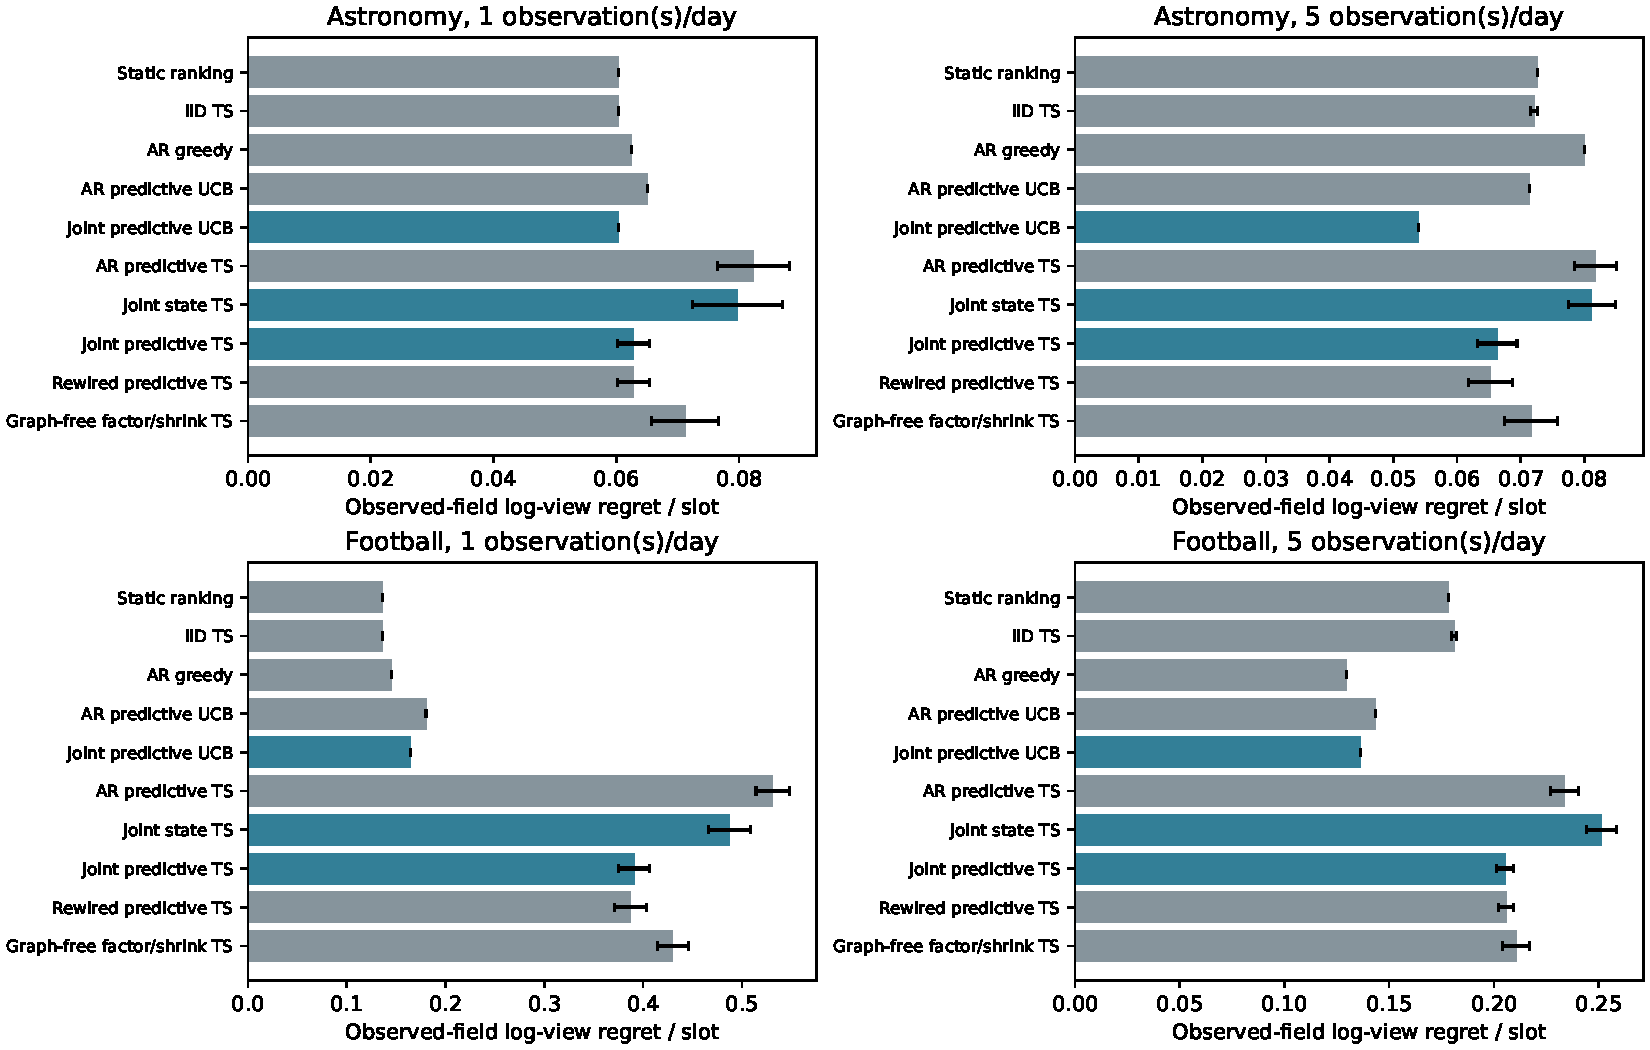
\includegraphics[width=\textwidth]{results/wikipedia/comparison.pdf}\caption{Completed Wikipedia AR(7) comparisons. Error bars are conditional 95\% Monte Carlo intervals over policy randomization on the same observed field; they are not population confidence intervals. Deterministic policies have no randomization interval.}\end{figure}

\begin{figure}[t]\centering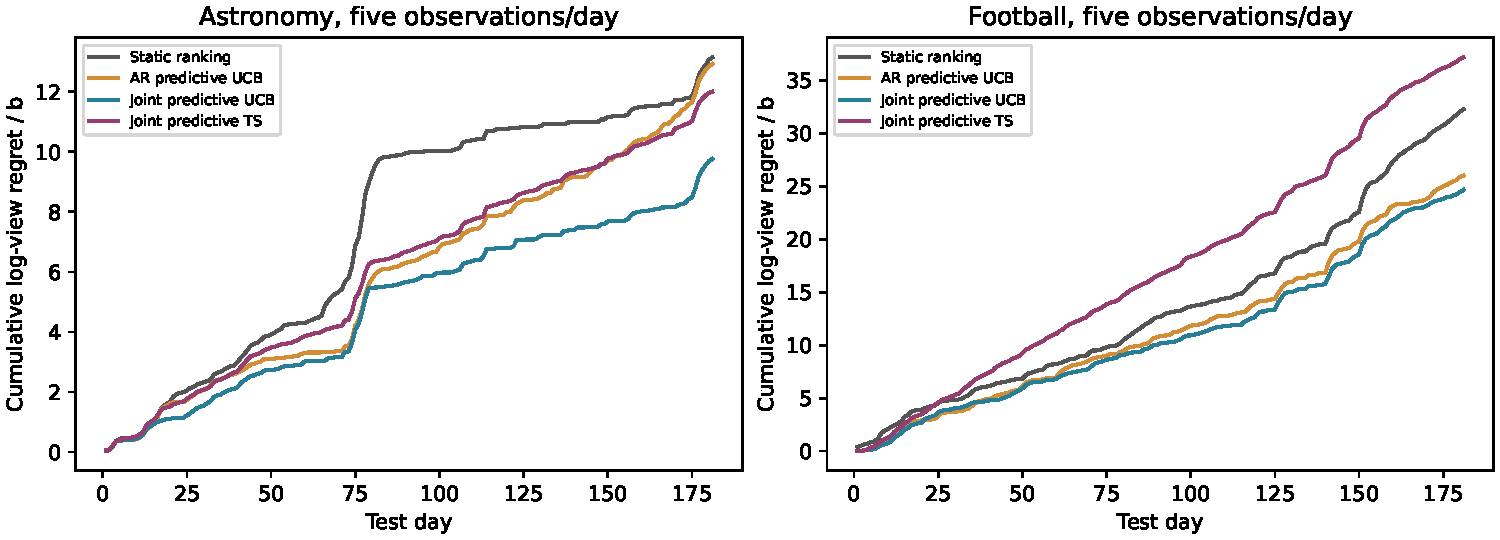
\includegraphics[width=\textwidth]{results/wikipedia/cumulative.pdf}\caption{Cumulative opportunity loss in the five-reading setting. One fixed test field per topic; no full-field test refresh is supplied to the learner.}\end{figure}

\subsection{What this application establishes}

A historical-graph, learned-general-AR selective-feedback study is feasible with a small data footprint and exact filtering. The outcomes also strengthen the negative controls: most apparent correlation benefit cannot be assigned to graph topology, and strong historical information can make simple static policies competitive. These conclusions are confined to two panels and the stated utility proxy. Raw-scale captured attention, conditional seed intervals, paired differences, monthly-block summaries, action traces and all fitted matrices are released; no theoretical floor or true stationary PCS is claimed for this real panel.


\section{Synthesis, practical implications and unresolved questions}

The results support objective-specific use of dependence. Persistent states can make a recently observed arm valuable for reward prediction while making its permanent mean difficult to identify. Correlated innovations can cancel in comparisons, but a graph that predicts permanent preferences need not predict transient shocks. The exact selected-history likelihood accounts for both effects without changing fixed physical means into a random population.

The strongest theoretical statements are conditional guarantees with explicit assumptions: graph-energy information geometry, predictable innovation regression, all-time fixed-mean confidence, correct stopping, a conservative mean-UCB bound, the current-oracle innovation floor, and exact restricted allocation cases. The strongest empirical statements are qualified by their designs: graph-free shrinkage accounts for much of KuaiRec's static gain; temporal modelling explains most of its daily pilot improvement; the fixed-truth AR(20) study shows different policy leaders for regret and selection; and the new Wikipedia evaluation tests learned general-AR models using genuinely historical graphs.

No graph benefit should be inferred from a joint-versus-iid comparison alone. The relevant test holds the temporal inference and decision rule fixed while comparing real topology with diagonal, common-factor, learned covariance and degree-preserving controls. A benefit in average prediction may also fail to change the top decision. Conversely, a small forecast improvement near a top-arm tie can have a useful decision effect.

Open theoretical questions include matching graph-and-time regret constants, finite-budget optimal contrast allocation, robust learned-model confidence, endogenous exposure and graph learning, and efficient long-horizon belief planning. Open application questions include identifying the actual observation cost, testing catalog births/deaths and drift, and validating whether measured attention is the intended business utility. Our public-data emulation provides counterfactual observed-field evaluation under selective masking; it does not constitute an online randomized platform deployment.

\section{Reproducibility and source provenance}

The package contains this manuscript, compiled PDF, editable sections, generated tables, raw Wikipedia API responses, historical revision identifiers and hashes, model matrices, daily action traces, per-run summaries, conditioning checks, and acquisition/run/analysis scripts. The evidence directory freezes compact source results and the five original technical derivations. Large original raw simulation runs are fingerprinted or linked rather than duplicated indiscriminately. The file \texttt{evidence\_manifest.json} records the source versions used in this synthesis.

The Wikipedia acquisition is sequential and cached, with an identifying user agent and rate-limit backoff. Page-view data use human traffic across access methods; missing dates are not filled with zero. Historical hyperlinks come only from revisions before 1 January 2024. The graph preserves isolated vertices and does not use current redirects to recover missing edges. Public attention data are CC0; revision material retains Wikipedia attribution/share-alike conditions and revision URLs.

The new experiment runs with one BLAS thread. Development is confined to 2024, and the final 2025 field is only exposed to the evaluation logger after each selected batch has been chosen. Code and source metadata disclose every fit, hyperparameter, privilege and numerical observation regularizer. Stochastic repeats quantify policy randomization on one realized panel, not population uncertainty across independent Web histories. The README supplies exact commands and a route for shrinking this reference manuscript into a venue-specific submission.

\clearpage
\appendix
\section{Complete fixed-mean spatial and heterogeneous-AR derivations}
\label{app:st}
This appendix preserves the current technical source, with its original assumptions and detailed proofs. Labels and references are namespaced. Its numerical experiments are the fixed-truth studies summarized in the main text.
\subsection{Introduction}
Choosing a business location using costly traffic measurements requires distinguishing permanent location quality from shared, persistent traffic fluctuations. A reading at one location can reveal a neighborhood shock and help forecast another location, even though both locations have fixed long-run means. General autoregressive dynamics also permit delayed and oscillatory dependence: an observation can be uninformative one period ahead and informative two periods ahead. A single persistence coefficient cannot capture that distinction.

We use fixed unknown constants $\mu_i$ and the model
\begin{equation}
\boxed{X_{i,t}-\mu_i
=\sum_{k=1}^{p_i}a_{i,k}(X_{i,t-k}-\mu_i)+\eta_{i,t},
\qquad \eta_t\stackrel{\mathrm{iid}}{\sim}N(0,Q_G).}
\label{spatiotemporal_bandits:eq:model}
\end{equation}
The AR polynomials are stable, the orders and coefficients are known, and $Q_G$ is a known positive definite covariance across locations. At each calendar time one chosen location is measured; all locations evolve whether measured or not. The mean vector is deterministic and may obey a supplied graph-energy bound.

This formulation keeps two spatial mechanisms separate. Correlated innovations explain shared transient deviations. A mean-energy restriction explains why neighboring permanent means should be similar. The first assumption alone does not imply the second. A covariance for $\eta_t$ does not make the fixed $\mu_i$ random or force them to be close.

We develop graph estimation using the trajectory likelihood, adaptive confidence, sampling for mean comparisons, and forecast information from complete impulse responses. The main terminal objective is selecting the largest permanent mean. Cumulative reward against a full-current-state oracle has a separate information limit.

\subsubsection{Existing research and contribution boundary}
Spectral bandits~\cite{collected1} and graph pure exploration~\cite{collected2} already exploit graph-smooth fixed means. Our mean-energy assumption follows that tradition; replacing independent noise with correlated AR observation error changes the trajectory likelihood and the information supplied by a schedule.

Time-varying Gaussian-process bandits~\cite{collected3} already combine spatial dependence with temporal evolution, and shared linear Gaussian bandits~\cite{collected4} already use one action's observations to predict another action's future rewards. General AR processes are finite-dimensional linear Gaussian systems after stacking lags. Kalman inference and that representation are established tools. Latent-AR bandits~\cite{collected5} further study shared temporal drivers and parameter learning.

Graph ARMA estimation~\cite{collected13} studies joint temporal and graph correlations for reconstruction. Our heterogeneous per-node AR coefficients need not be graph filters or share a graph Fourier eigenbasis. Spatial correlation is placed in the innovation covariance, while adaptive selection and comparison of fixed means are the decision tasks.

Correlated-normal knowledge gradient~\cite{collected6} uses Gaussian beliefs on means for final recommendations. A fixed physical parameter can be assigned a Bayesian belief. Our confidence results require no mean prior and report repeated-noise PCS at fixed truths. The randomized policies use algorithmic Gaussian uncertainty, equivalently a working Gaussian belief, without a random physical mean population. Our contrast rule uses regularized likelihood information, whose inverse is not interpreted as a mean-prior posterior covariance. Self-normalized concentration~\cite{collected7} and best-arm change of measure~\cite{collected11,collected12} supply the confidence and lower-bound arguments.

The contribution is a self-contained specialization connecting fixed graph-smooth means, correlated innovations, heterogeneous AR schedules, and adaptive information. We prove the stated estimation, confidence, information, and schedule-comparison results. We do not claim the first combination of spatial and temporal bandits, a generally optimal policy, matching sample complexity, learned graph validity, or unknown-dynamics guarantees.

\subsection{Fixed means and spatially correlated innovations}
There are $N$ arms and a supplied connected weighted graph with Laplacian $L$. Write $z_{i,t}=X_{i,t}-\mu_i$. The scalar polynomial
\[
A_i(s)=1-\sum_{k=1}^{p_i}a_{i,k}s^k
\]
has no zero in the closed unit disk, ensuring a causal stationary solution. Define $c_i=A_i(1)=1-\sum_k a_{i,k}\ne0$. In raw coordinates,
\begin{equation}
X_{i,t}=c_i\mu_i+\sum_k a_{i,k}X_{i,t-k}+\eta_{i,t}.
\end{equation}
Thus $\mu_i$ is the long-run mean; $c_i\mu_i$ is the AR intercept.

Innovation vectors are independent over time, but their coordinates can be correlated:
\begin{equation}
\Cov(\eta_{i,t},\eta_{j,s})=(Q_G)_{ij}\one\{t=s\}.
\end{equation}
A candidate graph covariance is $(\alpha_\eta I+\lambda_\eta L)^{-1}$, with $\alpha_\eta>0$, possibly rescaled to specified innovation variances. This models the shocks. It is not a distribution for $\mu$ or a hard energy bound on every shock realization. A mean graph and an innovation graph may differ; a common supplied graph is a substantive assumption.

Correlated shocks can improve prediction and comparison precision, but they do not identify an unrestricted mean at a never-measured arm: its column of $M$ is zero and its mean does not enter the observation likelihood. A separate mean restriction can bound or link that coordinate; innovation correlation alone cannot do so.

The fixed mean may satisfy
\begin{equation}
\mathcal M(S,B)=\{\mu:\mu^\top L\mu\le S^2,\ \|\mu\|_2\le B\}.
\label{spatiotemporal_bandits:eq:mean-class}
\end{equation}
The energy $\mu^\top L\mu=\sum_{\{i,j\}\in E}w_{ij}(\mu_i-\mu_j)^2$ constrains neighboring permanent differences. It does not assert a random covariance among fixed constants. The norm bound is used with a proper regularizer in the adaptive confidence theorem. A known common baseline can be subtracted without changing rankings or energy.

Choose a non-anticipating action $a_t$, then observe
\begin{equation}
Y_t=X_{a_t,t}+\xi_t,\qquad \xi_t\stackrel{\mathrm{iid}}{\sim}N(0,r),\quad r\ge0,
\end{equation}
with independent sensor noise. For a unique best mean $b^*=\argmax_i\mu_i$, define
\begin{equation}
\PCS_\mu(T)=\Pr_\mu(\widehat b_T=b^*),\qquad
\mathcal L_\mu(T)=\E_\mu[\mu_{b^*}-\mu_{\widehat b_T}].
\label{spatiotemporal_bandits:eq:target}
\end{equation}
Expectations are over observations and policy randomization at the same fixed $\mu$, not a mean prior.

\subsection{Joint lag state and nonseparable covariance}
Let $d=\sum_i p_i$. Stack each arm's centered current state and its $p_i-1$ lags into $s_t\in\mathbb R^d$. Let $F$ contain the AR companion blocks, $E\in\mathbb R^{d\times N}$ insert innovations into their first coordinates, and $C=E^\top$ select current coordinates. Then
\begin{equation}
s_{t+1}=Fs_t+E\eta_{t+1},\qquad z_t=Cs_t,\qquad X_t=\mu+Cs_t.
\label{spatiotemporal_bandits:eq:state}
\end{equation}
Although $F$ is block diagonal, $EQ_GE^\top$ couples arm-state covariances. Initialize $s_1\sim N(0,\Gamma)$, where
\begin{equation}
\Gamma=F\Gamma F^\top+EQ_GE^\top
=\sum_{h\ge0}F^hEQ_GE^\top(F^\top)^h.
\label{spatiotemporal_bandits:eq:lyapunov}
\end{equation}
Stability ensures convergence; positive definite innovations and the companion insertion structure make $\Gamma$ positive definite.

Define
\begin{equation}
G_h=CF^h\Gamma C^\top,\qquad h\ge0.
\label{spatiotemporal_bandits:eq:lags}
\end{equation}
For $t\ge s$, $\Cov(z_t,z_s)=G_{t-s}$; reverse-time covariance is its transpose. Heterogeneous $G_h$ need not be symmetric or equal a scalar temporal factor times a fixed spatial covariance.

If $z_{i,t}=\sum_{k\ge0}\psi_i(k)\eta_{i,t-k}$, then
\begin{equation}
\boxed{(G_h)_{ij}=(Q_G)_{ij}\sum_{k\ge0}\psi_i(k+h)\psi_j(k).}
\label{spatiotemporal_bandits:eq:impulses}
\end{equation}
The innovation distribution supplies spatial coupling; the arms' filters determine its lag profile. Only additional homogeneous-filter assumptions produce a separable covariance.

For a fixed schedule, let $M$ have rows $e_{a_t}^\top$. Its observation covariance is
\begin{equation}
\Xi_{ts}=
\begin{cases}
(G_{t-s})_{a_t,a_s},&t\ge s,\\
(G_{s-t})_{a_s,a_t},&t<s,
\end{cases}
\quad{}+r\one\{t=s\}.
\label{spatiotemporal_bandits:eq:xi}
\end{equation}
Thus $Y\sim N(M\mu,\Xi)$ for a fixed design. Conditioning repeated-sampling distributions on adaptive actions does not generally preserve that fixed-design Gaussian law.

\subsection{Estimating the fixed mean using spatial smoothness}
Set $\mathcal I=M^\top\Xi^{-1}M$ and $q=M^\top\Xi^{-1}Y$. For a deterministic regularizer $H\succeq0$ with $J=\mathcal I+H\succ0$,
\begin{equation}
\boxed{\widehat\mu_H
=\argmin_\nu\left\{\tfrac12(Y-M\nu)^\top\Xi^{-1}(Y-M\nu)
+\tfrac12\nu^\top H\nu\right\}=J^{-1}q.}
\label{spatiotemporal_bandits:eq:ridge}
\end{equation}
With $H=\lambda L$, spatial differences are penalized and a common offset is unpenalized. Connectivity and at least one observation make $J$ positive definite for $\lambda>0$. For adaptive confidence we use $H=\alpha I+\lambda L$, $\alpha>0$. Here $J^{-1}$ is an inverse regularized information matrix, not a declared covariance of a random mean.

\begin{proposition}[Fixed-design bias and variance]
For deterministic $H$ and a fixed design,
\begin{equation}
\E_\mu\widehat\mu_H-\mu=-J^{-1}H\mu,\qquad
\Var_\mu(\widehat\mu_H)=J^{-1}\mathcal I J^{-1}.
\label{spatiotemporal_bandits:eq:bias-var}
\end{equation}
For a contrast $v$, $H=\lambda L$, and $\mu^\top L\mu\le S^2$,
\begin{equation}
|v^\top(\E_\mu\widehat\mu_H-\mu)|
\le\lambda S\sqrt{v^\top J^{-1}LJ^{-1}v}.
\label{spatiotemporal_bandits:eq:bias-bound}
\end{equation}
A fixed-design $1-\delta$ contrast width is this bias allowance plus
$\Phi^{-1}(1-\delta/2)\sqrt{v^\top J^{-1}\mathcal I J^{-1}v}$.
\end{proposition}
\begin{proof}
The score is $\mathcal I\mu+M^\top\Xi^{-1}\epsilon$, with $\epsilon\sim N(0,\Xi)$. Substitution gives the estimator law. Graph bias is bounded by Cauchy--Schwarz for $L^{1/2}\mu$ and $L^{1/2}J^{-1}v$.
\end{proof}
Pairs use $v=e_i-e_j$. Smoothness bounds bias; it does not guarantee every smoothed ranking improves. A data-tuned penalty needs its own uncertainty argument.

\subsubsection{Literal enforcement of a supplied energy radius}
The constrained estimator is
\begin{equation}
\widehat\mu_S\in\argmin_{\nu^\top L\nu\le S^2}
\tfrac12(Y-M\nu)^\top\Xi^{-1}(Y-M\nu).
\end{equation}
For $S>0$, connected $L$, and at least one observation, a minimizer exists. The energy controls centered vectors; the observed fit controls the constant direction. Constant vectors satisfy Slater's condition. If no unconstrained minimizer is feasible, KKT gives
\begin{equation}
\widehat\mu_S=(\mathcal I+\lambda_*L)^{-1}q,\qquad
\widehat\mu_S^\top L\widehat\mu_S=S^2,\quad\lambda_*>0.
\end{equation}
Writing $\nu_\lambda=(\mathcal I+\lambda L)^{-1}q$ gives
\[
\frac{d}{d\lambda}(\nu_\lambda^\top L\nu_\lambda)
=-2\nu_\lambda^\top L(\mathcal I+\lambda L)^{-1}L\nu_\lambda\le0.
\]
A scalar bracketed search finds the active multiplier. A feasible unconstrained solution uses multiplier zero. This enforces the estimate's radius; it does not verify the radius at the truth. Its data-dependent multiplier is not automatically covered by the fixed-penalty Gaussian width.

Effective resistance also gives $|\mu_i-\mu_j|\le S\sqrt{(e_i-e_j)^\top L^\dagger(e_i-e_j)}$. This restriction on fixed means is independent of innovation correlation.

\subsection{Adaptive likelihood through a conditional lag-state filter}
Before decision $t$, conditional on a fixed candidate $\mu$, write
\begin{equation}
s_t\mid\mu,\mathcal H_t\sim N(g_t+D_t\mu,P_t).
\end{equation}
Initialize $g_1=0$, $D_1=0$, and $P_1=\Gamma$. For $\ell_a=C^\top e_a$, define
\begin{equation}
v_{t,a}=e_a+D_t^\top\ell_a,\quad
d_{t,a}=\ell_a^\top P_t\ell_a+r,\quad
u_{t,a}=v_{t,a}/\sqrt{d_{t,a}}.
\label{spatiotemporal_bandits:eq:experiment}
\end{equation}
\begin{theorem}[Predictable innovation experiments]
The chosen observation gives
\begin{equation}
\boxed{R_t=\frac{Y_t-\ell_{a_t}^\top g_t}{\sqrt{d_{t,a_t}}}
=u_t^\top\mu+\epsilon_t,\qquad
\epsilon_t\mid\mathcal H_t,a_t,\mu\sim N(0,1).}
\label{spatiotemporal_bandits:eq:regression}
\end{equation}
Its vector $u_t=u_{t,a_t}$ is predictable. With $k_t=P_t\ell_{a_t}/d_{t,a_t}$,
\begin{align}
g_t^+&=g_t+k_t(Y_t-\ell_{a_t}^\top g_t),&
D_t^+&=D_t-k_tv_{t,a_t}^\top,\nonumber\\
P_t^+&=P_t-\frac{P_t\ell_{a_t}\ell_{a_t}^\top P_t}{d_{t,a_t}},&
g_{t+1}&=Fg_t^+,\nonumber\\
D_{t+1}&=FD_t^+,&P_{t+1}&=FP_t^+F^\top+EQ_GE^\top.
\label{spatiotemporal_bandits:eq:filter}
\end{align}
The online information and score
\begin{equation}
\mathcal I_T=\sum_{t\le T}u_tu_t^\top,\qquad q_T=\sum_{t\le T}u_tR_t
\label{spatiotemporal_bandits:eq:online}
\end{equation}
agree algebraically with the dense likelihood for each recorded path.
\end{theorem}
\begin{proof}
The selected conditional mean is $\ell_a^\top g_t+v_{t,a}^\top\mu$ and its variance is $d_{t,a}$. Gaussian conditioning separates the state mean into its observable constant and coefficient of the fixed mean, giving the recursion. Companion propagation preserves the affine form. Its triangular innovation transform whitens the recorded covariance, giving the batch identities. Non-anticipating actions make the normalized design predictable. These pathwise identities do not imply fixed-design sampling laws conditional on adaptive actions.
\end{proof}

The scalar normalized error $\epsilon_t$ differs from the physical spatial innovation vector $\eta_t$. The latter has covariance $Q_G$ and drives every arm. The former is a selected-measurement residual after conditioning.

For $V_t=(H+\mathcal I_{t-1})^{-1}$ and $m_t=V_tq_{t-1}$, efficient estimator updates are
\begin{align}
V_t^+&=V_t-\frac{V_tu_tu_t^\top V_t}{1+u_t^\top V_tu_t},\nonumber\\
m_t^+&=m_t+\frac{V_tu_t(R_t-u_t^\top m_t)}{1+u_t^\top V_tu_t}.
\label{spatiotemporal_bandits:eq:update}
\end{align}
These are likelihood recursions without a mean prior. Temporal propagation changes future experiments but not accumulated static mean information.

\subsubsection{What a correlated second reading measures}
After measuring location $i$ at time one, consider location $j$ at time two. Let
\[
\gamma=\frac{(G_1)_{ji}}{(G_0)_{ii}+r},\qquad
d_2=(G_0)_{jj}+r-\frac{(G_1)_{ji}^2}{(G_0)_{ii}+r}.
\]
Then
\[
\frac{Y_2-\gamma Y_1}{\sqrt{d_2}}
=\frac{\mu_j-\gamma\mu_i}{\sqrt{d_2}}+\epsilon_2.
\]
Removing predictable shared noise also subtracts part of the first mean. The likelihood updates a weighted comparison, rather than treating the numerator as an unbiased reading of $\mu_j$. General AR dynamics can have $(G_1)_{ji}=0$ while $(G_2)_{ji}$ is large.

\subsection{Confidence, graph correctness, and stopping}
\begin{theorem}[All-time confidence at a fixed mean]
Suppose $\mu\in\mathcal M(S,B)$, $H=\alpha I+\lambda L\succ0$ and the graph are fixed before measurement, and the likelihood uses correct dynamics, $Q_G$, and $r$. Put
\begin{equation}
J_T=H+\mathcal I_T,\quad\widehat\mu_T=J_T^{-1}q_T,\quad
\beta_T=\sqrt{\log\frac{\det J_T}{\det H}+2\log\frac1\delta}
+\sqrt{\alpha B^2+\lambda S^2}.
\label{spatiotemporal_bandits:eq:beta}
\end{equation}
With probability at least $1-\delta$, for all $T\ge0$ and contrasts $v$ simultaneously,
\begin{equation}
\boxed{|v^\top(\widehat\mu_T-\mu)|\le\beta_T\sqrt{v^\top J_T^{-1}v}.}
\label{spatiotemporal_bandits:eq:confidence}
\end{equation}
\end{theorem}
\begin{proof}
Let $W_T=\sum_{t\le T}u_t\epsilon_t$. For deterministic $\theta$, the Gaussian exponential
$\exp\{\theta^\top W_T-\theta^\top\mathcal I_T\theta/2\}$ is a nonnegative martingale. Mixing $\theta$ with the Gaussian integration measure $N(0,H^{-1})$ gives
\[
Z_T=\sqrt{\frac{\det H}{\det J_T}}\exp\{\|W_T\|_{J_T^{-1}}^2/2\}.
\]
This mixing variable is a proof device, not a prior on $\mu$. The martingale crossing inequality bounds $Z_T$ by $1/\delta$ for all times outside an event of probability $\delta$, giving the square-root log-determinant term. This is established self-normalized concentration~\cite{collected7}. Also
\[
\widehat\mu_T-\mu=J_T^{-1}W_T-J_T^{-1}H\mu.
\]
Since $H\preceq J_T$, the regularization contribution in the $J_T$ norm is at most $\sqrt{\mu^\top H\mu}\le\sqrt{\alpha B^2+\lambda S^2}$. Contrast Cauchy--Schwarz completes the proof.
\end{proof}

\begin{corollary}[Correct stopped recommendation]
Recommend $\widehat b_T=\argmax_i\widehat\mu_{i,T}$ and stop only if every $j\ne\widehat b_T$ satisfies
\begin{equation}
\widehat\mu_{\widehat b_T,T}-\widehat\mu_{j,T}>
\beta_T\sqrt{(e_{\widehat b_T}-e_j)^\top J_T^{-1}(e_{\widehat b_T}-e_j)}.
\label{spatiotemporal_bandits:eq:stopping}
\end{equation}
The probability of an incorrect stopped recommendation is at most $\delta$.
\end{corollary}
\begin{proof}
On the simultaneous event every certified difference is positive at the truth. The event covers adaptive contrasts and stopping times.
\end{proof}
A forced terminal decision without a passed certificate has no such guarantee. This is fixed-confidence correctness, rather than finite-budget optimality.

\subsubsection{Termination for general stable AR dynamics}
Let
\[
a_{\min}=\min_{i,\omega}|A_i(e^{-{\rm i}\omega})|>0,\qquad
a_{\max}=\max_{i,\omega}|A_i(e^{-{\rm i}\omega})|<\infty,
\]
and
\begin{equation}
v_-=\lambda_{\min}(Q_G)/a_{\max}^2+r,\qquad
v_+=\lambda_{\max}(Q_G)/a_{\min}^2+r.
\end{equation}
The spectral covariance matrix is
\begin{equation}
\mathcal S_z(\omega)=
\operatorname{diag}(A_i(e^{-{\rm i}\omega})^{-1})Q_G
\operatorname{diag}(A_i(e^{-{\rm i}\omega})^{-1})^*.
\label{spatiotemporal_bandits:eq:spectrum}
\end{equation}
Its eigenvalues are bounded by the constants without $r$. Parseval's identity transfers them to finite block covariance; coordinate selection preserves them. For every realized design,
\begin{equation}
\boxed{\frac1{v_+}\operatorname{diag}(N_i(T))
\preceq\mathcal I_T\preceq\frac1{v_-}\operatorname{diag}(N_i(T)).}
\label{spatiotemporal_bandits:eq:information-bounds}
\end{equation}
If forced cyclic probes give every arm $n_T\ge cT-O(1)$ observations, pairwise squared widths are at most $2v_+/n_T$. Also
\[
\log(\det J_T/\det H)\le N\log\{1+T/(v_-\lambda_{\min}(H))\}.
\]
Thus confidence widths vanish. At a positive smallest gap, the stopping certificate eventually passes. Almost-sure termination follows by applying the estimator bound at arbitrary $\delta'>0$ and letting $\delta'$ decrease to zero. These conservative bounds do not determine optimal schedule-dependent allocation.

\subsubsection{What graph correctness permits}
Graph correctness means that a supplied graph actually restricts the fixed mean's differences. Usefulness means that the restriction excludes difficult competing mean vectors. It is not a claim of stochastic correlation among fixed constants.

If an external graph obeys
\[
(1-\zeta)L\preceq\widehat L\preceq(1+\zeta)L,\qquad0\le\zeta<1,
\]
then a truth with energy at most $S^2$ under $L$ has energy at most $(1+\zeta)S^2$ under $\widehat L$. Replacing the penalty by $\alpha I+\lambda\widehat L$ and bias allowance by $\sqrt{\alpha B^2+\lambda(1+\zeta)S^2}$ preserves confidence when the noise likelihood remains correct. The graph must be fixed before measurement or supplied by an independent experiment; same-data graph learning needs a uniform or selection-adjusted argument. Using an incorrect graph to fit $Q_G$ changes the likelihood and is not repaired by enlarging the mean-energy allowance.

\subsection{Sampling for permanent comparisons and predictions}
Adding a candidate normalized experiment to $J$ decreases inverse regularized information for contrast $v$ by exactly
\begin{equation}
\boxed{\mathcal G_t(v,a)=
\frac{(v^\top V_tu_{t,a})^2}{1+u_{t,a}^\top V_tu_{t,a}}.}
\label{spatiotemporal_bandits:eq:gain}
\end{equation}
This follows from Sherman--Morrison. It incorporates graph geometry through $V_t$ and spatial-temporal likelihood through $u_{t,a}$. It is not the actual frequentist variance reduction of a biased adaptive estimator.

Our implementable rule chooses the largest regularized mean, finds the challenger with the smallest standardized estimated gap, and measures the action maximizing~\eqref{spatiotemporal_bandits:eq:gain} for that pair. Forced probes ensure coverage; the stopping rule supplies a certificate when available. This is a heuristic: a single inverse-information reduction ignores other challengers, the changing determinant term, and future experiments. We assert no general PCS-optimality or finite-horizon regret theorem for it.

Conditional on a fixed $\mu$, measuring action $a$ reduces the variance of a future coordinate $z_{i,t+h}$ by
\begin{equation}
\boxed{\Delta_{i,h}(a)=
\frac{(e_i^\top CF^hP_t\ell_a)^2}{\ell_a^\top P_t\ell_a+r}.}
\label{spatiotemporal_bandits:eq:prediction-gain}
\end{equation}
For a future spatial contrast replace $e_i$ by $e_i-e_j$. Multiple future targets have the corresponding rank-one outer-product reduction. Future innovations are independent and do not change this reduction.

With unknown fixed means, the true conditional expected current field is $\mu+Cg_t+CD_t\mu$. The plug-in forecast substitutes $\widehat\mu_t$. Equation~\eqref{spatiotemporal_bandits:eq:confidence} bounds each linear mean contribution $(e_i+D_t^\top C^\top e_i)^\top(\widehat\mu_t-\mu)$, while $P_t$ describes state uncertainty conditional on $\mu$. These are separate uncertainty sources; $P_t$ alone does not cover mean-estimation error.

General AR prediction depends on $F^h$ and the complete lag-state covariance. Mean selection should value permanent comparisons; a reward policy must also value forecasts at its operating horizon.


\subsection{Objective-specific UCB and Thompson-style policies}
Let $b^*=\argmax_i\mu_i$. We distinguish four cumulative comparators:
\begin{align}
R_{\rm oracle}(T)&=\sum_{t\le T}(\max_iX_{i,t}-X_{a_t,t}),\nonumber\\
R_\mu(T)&=\sum_{t\le T}(\mu_{b^*}-\mu_{a_t}),\label{spatiotemporal_bandits:eq:three-regrets}\\
R_{\rm stationary}(T)&=T\mu_{b^*}-\sum_{t\le T}X_{a_t,t},\nonumber\\
R_{\rm fixed}(T)&=\sum_{t\le T}(X_{b^*,t}-X_{a_t,t}).\nonumber
\end{align}
Oracle regret and mean pseudo-regret are nonnegative pathwise. The two actual-reward comparators may be negative: adaptive actions can exploit positive predictable deviations. Since the deviation of the fixed arm has mean zero,
\begin{equation}
\E R_{\rm stationary}(T)=\E R_{\rm fixed}(T)
=\E R_\mu(T)-\sum_{t\le T}\E z_{a_t,t}.
\end{equation}
Even the full-current-state oracle can have positive mean pseudo-regret. Terminal PCS instead compares the recommendation's permanent mean with $\mu_{b^*}$.

\subsubsection{A shared inference engine}
For observations strictly before decision $t$, write their design, covariance and readings as $M,\Xi,Y$. Define
\begin{align}
V&=(H+M^\top\Xi^{-1}M)^{-1},&m&=VM^\top\Xi^{-1}Y,\nonumber\\
K&=\Cov(z_t,\hbox{selected past deviations}),&A&=K\Xi^{-1},\nonumber\\
W&=I-AM,&f&=AY+Wm,\label{spatiotemporal_bandits:eq:forecast-working}\\
P&=G_0-K\Xi^{-1}K^\top,&\Sigma&=P+WVW^\top.\nonumber
\end{align}
At the true fixed mean, the conditional expected field is $AY+W\mu$, with conditional noise covariance $P$. The matrix $\Sigma$ is a working Gaussian uncertainty for randomized decisions; $V$ remains inverse penalized information, not the repeated-noise sampling covariance. A Gaussian integration of the penalized likelihood produces these same working quantities, without specifying a random physical mean population. Correct frequentist uncertainty uses~\eqref{spatiotemporal_bandits:eq:confidence}, including its regularization allowance.

The selected-history implementation updates $\Xi^{-1}$ by its Schur complement. It is algebraically equivalent to the affine state filter, retains the full AR likelihood, and uses $O(T^2)$ history storage, $O(Nt^2)$ all-arm forecast work, and $O(t^2+N^2)$ selected-update work. The lag-state alternative has dimension $\sum_i p_i$. Neither is a constant-cost solution as all dimensions grow.

\subsubsection{Permanent-mean UCB and a regret bound}
Mean UCB chooses
\begin{equation}
a_t=\argmax_i\{m_i+c_t\sqrt{V_{ii}}\}.
\label{spatiotemporal_bandits:eq:mean-ucb}
\end{equation}
The certified version uses $c_t=\beta_{t-1}(\delta)$. The practical version uses $c_t=.7\sqrt{2\log(t+1)}$ for one-based decisions. The practical scale has no automatic coverage claim.

After initially measuring each arm, force cyclic probes at square calendar ages: if $t-N=k^2$ for $k\ge1$, select $(k-1)\bmod N$. Other rounds use the policy. Thus the forced count satisfies $F_T\le N+\sqrt T$, and each arm receives $\Omega(\sqrt T/N)$ forced samples eventually.

\begin{theorem}[Conservative stationary mean-regret guarantee]
Under the assumptions of the confidence theorem and the spectral covariance bounds~\eqref{spatiotemporal_bandits:eq:information-bounds}, certified mean UCB with the preceding probes obeys, with probability at least $1-\delta$,
\begin{equation}
\boxed{R_\mu(T)\le 2BF_T+4\beta_T\sqrt{v_+NT}.}
\label{spatiotemporal_bandits:eq:mean-regret-bound}
\end{equation}
Moreover,
\[
\beta_T\le\sqrt{N\log(1+T/(\alpha v_-))+2\log(1/\delta)}
+\sqrt{\alpha B^2+\lambda S^2}.
\]
This bound is sublinear for fixed $N$ and fixed stable dynamics. It does not claim sharp graph or temporal constants.
\end{theorem}
\begin{proof}
On the simultaneous confidence event, optimism bounds every ordinary action's gap:
\[
\mu_{b^*}-\mu_{a_t}\le2\beta_{t-1}\sqrt{V_{a_ta_t}}.
\]
After initial coverage, the information sandwich gives $V_{ii}\le v_+/N_i(t-1)$. Summing inverse square-root counts over ordinary rounds gives
\[
\sum_{t:\,\text{ordinary}}N_{a_t}(t-1)^{-1/2}
\le2\sum_i\sqrt{N_i(T)}\le2\sqrt{NT}.
\]
Forced actions cost at most $2B$ each. The determinant bound follows from $H\succeq\alpha I$ and the upper information bound.
\end{proof}
An expectation bound adds $2BT\delta$; choosing $\delta=1/T$ in a horizon-specific policy makes that remainder bounded. The experiment uses $\delta=.05$ for the certified policy. Because minimum forced counts grow as $\sqrt T$, the confidence widths vanish as $O(\sqrt{\log T}/T^{1/4})$ for fixed dimensions. Applying the confidence theorem with arbitrarily small failure probabilities gives consistent mean estimates and PCS tending to one at a positive fixed gap for every correctly specified joint policy with these probes. This asymptotic statement is not a finite-budget PCS guarantee.



\subsubsection{Current-reward optimism and predictable-state sampling}
The full-variance reward heuristic selects $\argmax_i\{f_i+c_t\sqrt{\Sigma_{ii}}\}$. A more targeted rule replaces $\Sigma$ by $\Sigma-Q_G$. Indeed,
\[
z_t=CFs_{t-1}+\eta_t,\qquad
P-Q_G=\Var(CFs_{t-1}\mid\mathcal H_t,\mu)\succeq0.
\]
The fresh innovation is independent of every past reading. Sampling can reveal permanent means and past lag states, but cannot predict that current innovation. Removing it from the exploration variance retains all learnable state and mean uncertainty. With zero temporal dependence, this predictive rule reduces to a mean rule.

A conservative upper bound covering actual current rewards uses
\begin{equation}
U_{i,t}=f_i+\beta_{t-1}(\delta/2)\sqrt{W_iVW_i^\top}
+\kappa_t\sqrt{P_{ii}},\qquad
\kappa_t=\sqrt{2\log\{2\pi^2Nt^2/(3\delta)\}}.
\end{equation}
The mean confidence event and a conditional two-sided Gaussian tail union bound give $|X_{i,t}-f_i|\le U_{i,t}-f_i$ simultaneously with probability at least $1-\delta$. On non-forced rounds choosing the largest $U_{i,t}$ gives oracle regret at most twice the selected width. Forced rounds contribute their realized oracle gap separately. Since $P\succeq Q_G$, this bound does not remove the irreducible linear oracle term and need not be sharp. The experiment evaluates the practical full and predictive variance rules, not this conservative current-field certificate.

\subsubsection{Correlated Gaussian perturbations}
Mean Thompson-style sampling draws $\widetilde\mu=m+\tau V^{1/2}\xi$, $\xi\sim N(0,I)$, and chooses its largest coordinate. Full-state sampling draws $f+\tau \Sigma^{1/2}\xi$, while predictable-state sampling draws
\begin{equation}
\widetilde f=f+\tau(\Sigma-Q_G)^{1/2}\xi.
\end{equation}
All joint draws preserve spatial covariance. The experiment uses $\tau=1$. These are algorithmic uncertainty draws at a fixed physical truth. Their covariance does not by itself calibrate regularization bias or adaptive frequentist uncertainty.

Randomized optimistic linear policies~\cite{collected8} motivate the construction. Their regret results do not automatically transfer: the whitened information vector differs from the physical mean reward coordinate, and the forecast experiment changes with the observation history. The predictive variant is a one-step rule, distinct from future-information Predictive Sampling~\cite{collected10}. It can undervalue readings whose benefit occurs only at later AR lags. No optimal restless-bandit control result or Thompson regret theorem is asserted.

\subsubsection{Two PCS-oriented designs}
Put $B_{\rm cross}=VW^\top$. For a permanent contrast $c$, measuring arm $a$ decreases $c^\top Vc$ by
\begin{equation}
g_t(c,a)=\frac{(c^\top B_{{\rm cross},:,a})^2}{\Sigma_{aa}+r}.
\end{equation}
Contrast LUCB takes $b=\argmax_i m_i$ and chooses
\[
j=\argmax_{j\ne b}\left\{m_j-m_b+c_t\sqrt{(e_b-e_j)^\top V(e_b-e_j)}\right\}.
\]
It measures the arm maximizing $g_t(e_b-e_j,a)$. This is a UCB challenger variant of the earlier standardized-gap rule.

Top-two Thompson contrast design draws a plausible mean winner $b$ and redraws until a different winner $j$ appears. It caps this search at 64 draws, using the LUCB challenger as fallback, and maximizes the same contrast gain. A third location can be the selected measurement. The design is inspired by top-two sampling~\cite{collected9}, but differs in correlated draws, indirect observations, and time-varying information. Published asymptotic optimality is not imported. Both rules recommend the largest permanent estimate at the budget and remain finite-budget PCS heuristics.



\subsection{Fixed-mean PCS and an exact AR(2) design comparison}
For a fixed full-rank design, $\widehat\mu_{\rm GLS}\sim N(\mu,\mathcal I_T^{-1})$. PCS for its largest coordinate is a Gaussian orthant probability. If $W=\mathcal I_T^{-1}$, difference covariance between challengers $j,k$ of the true best $b$ is $W_{bb}-W_{bj}-W_{bk}+W_{jk}$. Correlation generally precludes the independent-arm product formula.

For two arms with fixed true gap $\Delta>0$,
\begin{equation}
\boxed{\PCS_\mu(T)=\Phi\left(
\frac{\Delta}{\sqrt{(e_1-e_2)^\top\mathcal I_T^{-1}(e_1-e_2)}}\right).}
\label{spatiotemporal_bandits:eq:fixed-pcs}
\end{equation}
This is fixed-truth, fixed-design PCS without a mean prior. Graph ridge also changes the Gaussian numerator through bias; adaptive schedules do not generally admit this fixed-design sampling law.

\begin{proposition}[Correlated AR(2) blocks improve selection]
Let two arms follow
\begin{equation}
z_{i,t}=a z_{i,t-2}+\eta_{i,t},\qquad
Q_G=V(1-a^2)\begin{pmatrix}1&\rho\\\rho&1\end{pmatrix},
\quad0<a<1,\quad0\le\rho<1.
\label{spatiotemporal_bandits:eq:lag-two}
\end{equation}
Both stationary marginal variances equal $V$. For four calendar measurements with sensor variance $r$, GLS difference variances are
\begin{equation}
\boxed{\sigma^2_{\rm AABB}=V+r-a\rho V,\qquad
\sigma^2_{\rm ABAB}=V+r+aV.}
\label{spatiotemporal_bandits:eq:design-variance}
\end{equation}
AABB has strictly larger fixed-mean PCS than ABAB for every $\Delta>0$.
\end{proposition}
\begin{proof}
Odd-lag covariances vanish and $G_{2k}=a^kV\begin{pmatrix}1&\rho\\\rho&1\end{pmatrix}$. In AABB each arm's consecutive readings are independent, while readings two rounds apart on different arms have covariance $a\rho V$. Per-arm averages are GLS estimates, giving difference variance $V+r-a\rho V$. In ABAB each arm's readings have covariance $aV$, while cross-arm reading covariances vanish at odd gaps. GLS again averages each arm, giving variance $V+r+aV$. Equation~\eqref{spatiotemporal_bandits:eq:fixed-pcs} gives the ordering.
\end{proof}

For $V=1$, $r=.1$, $a=.8$, $\rho=.6$, and fixed gap $\Delta=.4$, variances are $.62$ and $1.90$, with PCS approximately $.6943$ and $.6142$. The gain combines reduced within-arm redundancy and cancellation of shared shocks at informative lags. It does not establish a universally optimal four-step adaptive policy.

\begin{figure}[t]
\centering
\begin{tikzpicture}
\begin{axis}[width=.82\textwidth,height=5cm,xlabel={Spatial innovation correlation $\rho$},
ylabel={Fixed-mean PCS},xmin=0,xmax=.95,ymin=.59,ymax=.76,
legend pos=north west,grid=major]
\addplot[blue,thick] table[col sep=comma,x=rho,y=pcs_aabb]{evidence/spatiotemporal_bandits/results/general_ar/pcs_schedule.csv};
\addlegendentry{AABB}
\addplot[orange,thick] table[col sep=comma,x=rho,y=pcs_abab]{evidence/spatiotemporal_bandits/results/general_ar/pcs_schedule.csv};
\addlegendentry{ABAB}
\end{axis}
\end{tikzpicture}
\caption{Exact fixed-mean GLS selection for the lag-two process at $V=1$, $r=.1$, $a=.8$, and $\Delta=.4$. Correlated innovations further help the block comparison; alternating samples do not access cross-arm correlation at even lags.}
\label{spatiotemporal_bandits:fig:pcs}
\end{figure}

Two readings of different arms at consecutive times have raw difference variance $(G_0)_{11}+(G_0)_{22}+2r-2(G_1)_{21}$. General AR coefficients determine it, without a universal scalar persistence replacement.

\subsection{Full-field information and long-run covariance}
A stronger feedback benchmark measures every arm exactly each calendar time, costing $Nn$ scalar readings. Put $p=\max_i p_i$, pad coefficients to order $p$, and write $D_c=\operatorname{diag}(c_i)$.

\begin{proposition}[General full-field information]
For $n\ge p$ noiseless full fields, let $\mathcal I_p$ be the stationary mean information in the first $p$ fields. Then
\begin{equation}
\boxed{\mathcal I_n=\mathcal I_p+(n-p)D_cQ_G^{-1}D_c.}
\label{spatiotemporal_bandits:eq:full-field}
\end{equation}
The long-run covariance of the sample-mean field is
\begin{equation}
\boxed{\mathcal K_{\rm LR}=D_c^{-1}Q_GD_c^{-1}.}
\label{spatiotemporal_bandits:eq:long-run}
\end{equation}
\end{proposition}
\begin{proof}
After the initial $p$ fields, the innovation transform is
\[
X_t-\sum_{k=1}^p\operatorname{diag}(a_{i,k})X_{t-k}=D_c\mu+\eta_t.
\]
It has parameter-independent triangular Jacobian. Innovations are independent of the initial fields and of each other, so each adds information $D_cQ_G^{-1}D_c$. Evaluating the spectral covariance at zero frequency gives the long-run covariance; stable AR covariance sequences are absolutely summable.
\end{proof}

The identity permits different orders without a separable temporal kernel. For common coefficients, $D_c=cI$. If additionally $Q_G$ shares $L$'s eigenvectors, asymptotic information in graph mode $k$ is $nc^2/q_k$, and a Laplacian penalty adds $\lambda\ell_k$. Under heterogeneity these matrices generally do not commute.

Small $c_i$ makes permanent-mean estimation difficult even when recent data predict near-future rewards well. In the lag-two example, $c_i=1-a$ and long-run marginal variance is $V(1+a)/(1-a)$, although lag-one prediction gain vanishes.

\subsection{Information limits and the reward comparator}
For fixed means $\mu,\nu$ under a finite-horizon non-anticipating policy,
\begin{equation}
\boxed{\KL(P_\mu^{\pi,T},P_\nu^{\pi,T})
=\tfrac12\E_\mu[(\mu-\nu)^\top\mathcal I_T(\mu-\nu)].}
\label{spatiotemporal_bandits:eq:kl}
\end{equation}
Action probabilities cancel; each conditional Gaussian divergence is $(u_t^\top(\mu-\nu))^2/2$. If the recommendation is $\delta$-correct at both means and their unique best arms differ, data processing gives
\[
\tfrac12\E_\mu[(\mu-\nu)^\top\mathcal I_T(\mu-\nu)]
\ge\operatorname{kl}(1-\delta,\delta),\qquad\delta<1/2.
\]
Trusted graph restrictions reduce the alternative set, while AR schedules alter its information separation. This is established change-of-measure reasoning~\cite{collected11,collected12}; no matching attainable information program is proved here.

For cumulative reward put $K_0=C\Gamma C^\top$ and $\mathcal G(\mu,K)=\E\max_i(\mu_i+Z_i)$, $Z\sim N(0,K)$. A genie seeing the complete past lag-state lacks only the current innovation, and its predictive-mean covariance is $K_0-Q_G=CF\Gamma F^\top C^\top$. Consequently
\begin{equation}
\boxed{R_T^\pi\ge
T\{\mathcal G(\mu,K_0)-\mathcal G(\mu,K_0-Q_G)\}.}
\end{equation}
The genie is stronger than the learner; its maximum conditional mean bounds any causal expected reward. Convexity yields a nonnegative coefficient, strictly positive for nondegenerate contrast innovations when $Q_G\succ0$. At initialization the genie can be granted an additional stationary past state. This linear full-current-state-oracle regret obstruction does not prevent consistent fixed-mean selection.

\subsection{Experiments with fixed means and higher orders}
The six arms form a path, with two fixed mean vectors:
\[
\mu^{\rm smooth}=(0,.2,.45,.65,.75,.7),\qquad
\mu^{\rm rough}=(0,.65,.2,.75,.1,.7).
\]
Each is held fixed across repeated-noise runs. Innovations have covariance $.25$ times a diagonally normalized path resolvent $(I+2L)^{-1}$. Sensor variance is $.1$; the mean penalty is $H=.05I+.5L$. The fixed supplied bounds $B=2$, $S=2$ contain both means.

Three dynamics configurations are used:
\begin{itemize}
\item Lag-two: every arm has coefficients $(0,.75)$.
\item Oscillatory: every arm has coefficients $(.7,-.45)$.
\item Heterogeneous: $(.6,-.2)$, $(.35,.1,.2)$, $(0,.75)$, $(.1,.4,-.1)$, $(.7,-.3)$, and $(.2,0,.45)$.
\end{itemize}
All substantive AR processes have order two or three. Each configuration uses 200 paired independent noise trajectories and 60 measurements; policies share latent paths and potential readings within a run.

Seven policies are compared. Graph--AR contrast uses correct joint dynamics and the mean graph. Unstructured--AR removes the Laplacian penalty. Diagonal-noise--AR removes innovation cross-covariances while retaining marginal variances. Wrong-mean-graph--AR permutes the mean graph and retains correct noise. Graph--iid discards temporal dependence while matching stationary marginal observation covariance. Round robin cycles one reading per location; block cyclic measures each location for $p$ consecutive rounds. Adaptive rules force a cyclic probe every seven rounds.

Policies recommend their largest regularized mean. Reported PCS is repeated-noise success at a fixed truth. The confidence audit tests graph--AR contrast with the supplied bounds, repeating per-configuration coverage and certificate rates in CSV rows. An unpassed terminal certificate gives no fixed-confidence guarantee. Graph variants are estimator stress tests, not demonstrations of learning graph validity.

\begin{table}[p]
\centering\scriptsize

\begin{tabular}{lllrrr}
\toprule
Dynamics & Mean & Policy & Loss & PCS & MSE \\
\midrule
lag two & smooth & Graph--AR contrast & 0.068 & 0.420 & 0.143 \\
lag two & smooth & Unstructured--AR & 0.075 & 0.405 & 0.187 \\
lag two & smooth & Graph--iid contrast & 0.103 & 0.365 & 0.165 \\
lag two & smooth & Round robin & 0.079 & 0.380 & 0.109 \\
lag two & smooth & Block cyclic & 0.072 & 0.415 & 0.076 \\
lag two & rough & Graph--AR contrast & 0.051 & 0.360 & 0.149 \\
lag two & rough & Unstructured--AR & 0.061 & 0.365 & 0.177 \\
lag two & rough & Graph--iid contrast & 0.063 & 0.345 & 0.164 \\
lag two & rough & Round robin & 0.098 & 0.335 & 0.119 \\
lag two & rough & Block cyclic & 0.058 & 0.380 & 0.083 \\
oscillatory & smooth & Graph--AR contrast & 0.039 & 0.455 & 0.090 \\
oscillatory & smooth & Unstructured--AR & 0.051 & 0.415 & 0.112 \\
oscillatory & smooth & Graph--iid contrast & 0.056 & 0.420 & 0.097 \\
oscillatory & smooth & Round robin & 0.067 & 0.360 & 0.051 \\
oscillatory & smooth & Block cyclic & 0.057 & 0.375 & 0.060 \\
oscillatory & rough & Graph--AR contrast & 0.035 & 0.470 & 0.092 \\
oscillatory & rough & Unstructured--AR & 0.032 & 0.520 & 0.117 \\
oscillatory & rough & Graph--iid contrast & 0.039 & 0.455 & 0.096 \\
oscillatory & rough & Round robin & 0.041 & 0.415 & 0.054 \\
oscillatory & rough & Block cyclic & 0.048 & 0.385 & 0.059 \\
heterogeneous & smooth & Graph--AR contrast & 0.058 & 0.380 & 0.107 \\
heterogeneous & smooth & Unstructured--AR & 0.070 & 0.370 & 0.128 \\
heterogeneous & smooth & Graph--iid contrast & 0.062 & 0.380 & 0.107 \\
heterogeneous & smooth & Round robin & 0.076 & 0.355 & 0.057 \\
heterogeneous & smooth & Block cyclic & 0.064 & 0.420 & 0.061 \\
heterogeneous & rough & Graph--AR contrast & 0.048 & 0.390 & 0.105 \\
heterogeneous & rough & Unstructured--AR & 0.040 & 0.425 & 0.124 \\
heterogeneous & rough & Graph--iid contrast & 0.052 & 0.400 & 0.108 \\
heterogeneous & rough & Round robin & 0.068 & 0.440 & 0.056 \\
heterogeneous & rough & Block cyclic & 0.048 & 0.420 & 0.063 \\
\bottomrule
\end{tabular}


\caption{Fixed-mean selection over 200 paired noise runs per configuration, six arms, and budget 60. Loss is opportunity loss; PCS is repeated-noise recommendation accuracy. Full CSVs include omitted graph and noise baselines, standard errors, paired comparisons, and confidence audits.}
\label{spatiotemporal_bandits:tab:results}
\end{table}

For lag-two dynamics and smooth fixed means, graph--AR contrast gives opportunity loss $.0675$, versus $.1030$ for the iid likelihood; the paired improvement is $.0355$ with approximate 95\% half-width $.0193$. For oscillatory rough means, unstructured--AR gives PCS $.520$ versus $.470$ for the graph rule, although graph MSE is smaller ($.0917$ versus $.1166$). At lag-two smooth means, block cyclic gives overall MSE $.0757$ versus $.1426$ for the graph contrast policy, despite slightly greater selection loss. These examples distinguish estimation and selection objectives.

All 1,200 graph-policy noise trajectories satisfy the audited confidence bound, but no terminal certificate passes at budget 60. The conservative theorem therefore provides no certificate for these fixed-budget recommendations. Paired uncertainty is reported instead of claiming uniform superiority. The exact AR(2) result compares two designs; the six-arm policies are heuristics. The two mean profiles also have different gaps, so they do not isolate a monotone alignment effect at fixed decision difficulty.

The revised script passes 1,525 counted assertions. Recursive information, scores, and estimates agree with independent dense trajectory likelihoods. A stationary Lyapunov solve agrees with an independently summed impulse-response covariance. Mixed-order full-field information and certified spectral bounds are checked. Dense GLS validates the AR(2) schedule comparison; 30,000 paired direct process simulations at the same fixed mean vector agree with its PCS formulas within Monte Carlo uncertainty.


\subsection{One hundred arms with AR(20): regret and PCS}
We evaluate the objective-specific policies on a $10\times10$ grid. The same deterministic two-peak mean surface is held fixed across configurations and noise replicates; the best-minus-second gap is $.20$, its norm is $3.807$, and its graph energy is $3.672$. Supplied bounds $B=6$, $S=3$ contain this truth. The mean regularizer is $H=.1I+.5L$ and the sensor variance is $.09$.

Innovation spatial correlation is the diagonally normalized resolvent $(I+3L)^{-1}$. Innovation scales are chosen so every marginal stationary deviation variance is one. Each arm has order 20. The configurations are:
\begin{itemize}
\item Persistent: $a_k$ proportional to $\exp(-k/6)$, with coefficient sum $.95$.
\item Weak: the same lag shape with coefficient sum $.35$.
\item Lag 20: $a_{20}=.85$ and the other coefficients are zero.
\item Heterogeneous: cyclic assignment of the persistent filter, a positive filter proportional to $\exp(-k/3)$ with sum $.65$, and alternating coefficients proportional to $(-1)^k\exp(-k/6)$ with absolute sum $.80$.
\item Independent shocks: the persistent filter with diagonal innovation covariance, retaining the same fixed mean surface and mean graph.
\end{itemize}
All filters are stable. Heterogeneous stationary cross-covariances use the pairwise companion Lyapunov equations; a separable covariance is not substituted.

There are 32 independent noise worlds per configuration, 1,000 calendar decisions per world, 14 learning rules, and four information benchmarks. Policies share the complete latent path and potential sensor readings within a world, but see only their selected reading after choosing. All learning rules initially measure each arm and then use square-age probes; round robin retains its strict cyclic schedule. The budget includes initial coverage. Gaussian policy draws use separate reproducible seeds. Practical UCB scale $.7$ and Thompson scale one are fixed across configurations.

Benchmarks always choose the true best-mean arm, greedily filter with known means and bandit readings, observe all past lag states, or observe all current rewards. The known-mean greedy filter is not an optimal causal policy. The past-state genie chooses the largest current conditional mean and lacks only fresh innovations. Known-mean benchmarks have artificial PCS one and are excluded from learning-policy PCS comparisons.

\begin{table}[p]
\centering\scriptsize

\begin{tabular}{llrrr}
\toprule
Dynamics & Policy & Oracle/$T$ & Mean/$T$ & PCS\\
\midrule
Persistent & IID UCB & 1.397 & 0.668 & 0.188\\
 & Independent AR UCB & 1.429 & 0.701 & 0.250\\
 & Joint mean UCB & 1.453 & 0.680 & 0.125\\
 & Joint predictive UCB & 1.426 & 0.715 & 0.125\\
 & Joint full-state UCB & 1.248 & 0.686 & 0.219\\
 & Joint predictive TS & 1.675 & 0.768 & 0.219\\
 & Contrast LUCB & 1.646 & 0.734 & 0.188\\
 & Top-two contrast TS & 2.064 & 0.809 & 0.250\\
\midrule
Weak & IID UCB & 2.131 & 0.607 & 0.719\\
 & Independent AR UCB & 1.890 & 0.367 & 0.656\\
 & Joint mean UCB & 1.994 & 0.487 & 0.812\\
 & Joint predictive UCB & 2.008 & 0.493 & 0.906\\
 & Joint full-state UCB & 1.838 & 0.321 & 0.531\\
 & Joint predictive TS & 2.160 & 0.608 & 0.719\\
 & Contrast LUCB & 2.088 & 0.570 & 0.844\\
 & Top-two contrast TS & 2.251 & 0.710 & 0.781\\
\midrule
Lag 20 & IID UCB & 2.160 & 0.622 & 0.531\\
 & Independent AR UCB & 1.841 & 0.545 & 0.656\\
 & Joint mean UCB & 1.943 & 0.427 & 0.688\\
 & Joint predictive UCB & 1.838 & 0.549 & 0.750\\
 & Joint full-state UCB & 1.760 & 0.534 & 0.688\\
 & Joint predictive TS & 2.230 & 0.773 & 0.562\\
 & Contrast LUCB & 2.025 & 0.502 & 0.844\\
 & Top-two contrast TS & 2.269 & 0.715 & 0.719\\
\midrule
Heterogeneous & IID UCB & 1.717 & 0.705 & 0.000\\
 & Independent AR UCB & 1.725 & 0.518 & 0.406\\
 & Joint mean UCB & 1.659 & 0.624 & 0.125\\
 & Joint predictive UCB & 1.617 & 0.700 & 0.250\\
 & Joint full-state UCB & 1.647 & 0.397 & 0.469\\
 & Joint predictive TS & 1.897 & 0.758 & 0.344\\
 & Contrast LUCB & 1.817 & 0.605 & 0.406\\
 & Top-two contrast TS & 2.211 & 0.751 & 0.562\\
\midrule
Independent shocks & IID UCB & 1.453 & 0.582 & 0.188\\
 & Independent AR UCB & 1.381 & 0.640 & 0.281\\
 & Joint mean UCB & 1.506 & 0.498 & 0.281\\
 & Joint predictive UCB & 1.491 & 0.633 & 0.375\\
 & Joint full-state UCB & 1.270 & 0.583 & 0.312\\
 & Joint predictive TS & 1.767 & 0.711 & 0.250\\
 & Contrast LUCB & 1.691 & 0.581 & 0.250\\
 & Top-two contrast TS & 2.151 & 0.724 & 0.375\\
\bottomrule
\end{tabular}


\caption{AR(20), 100 arms, budget 1,000, and 32 paired noise worlds per configuration. Oracle and permanent mean pseudo-regret are per decision; PCS targets the fixed best mean. Selected policies are shown; CSVs report all policies, Student-$t$ mean intervals, Wilson PCS intervals, actual best-mean-arm reward regret, MSE, and paired differences. Observed rankings are not simultaneous statistical claims.}
\label{spatiotemporal_bandits:tab:ar20}
\end{table}

\begin{figure}[p]
\centering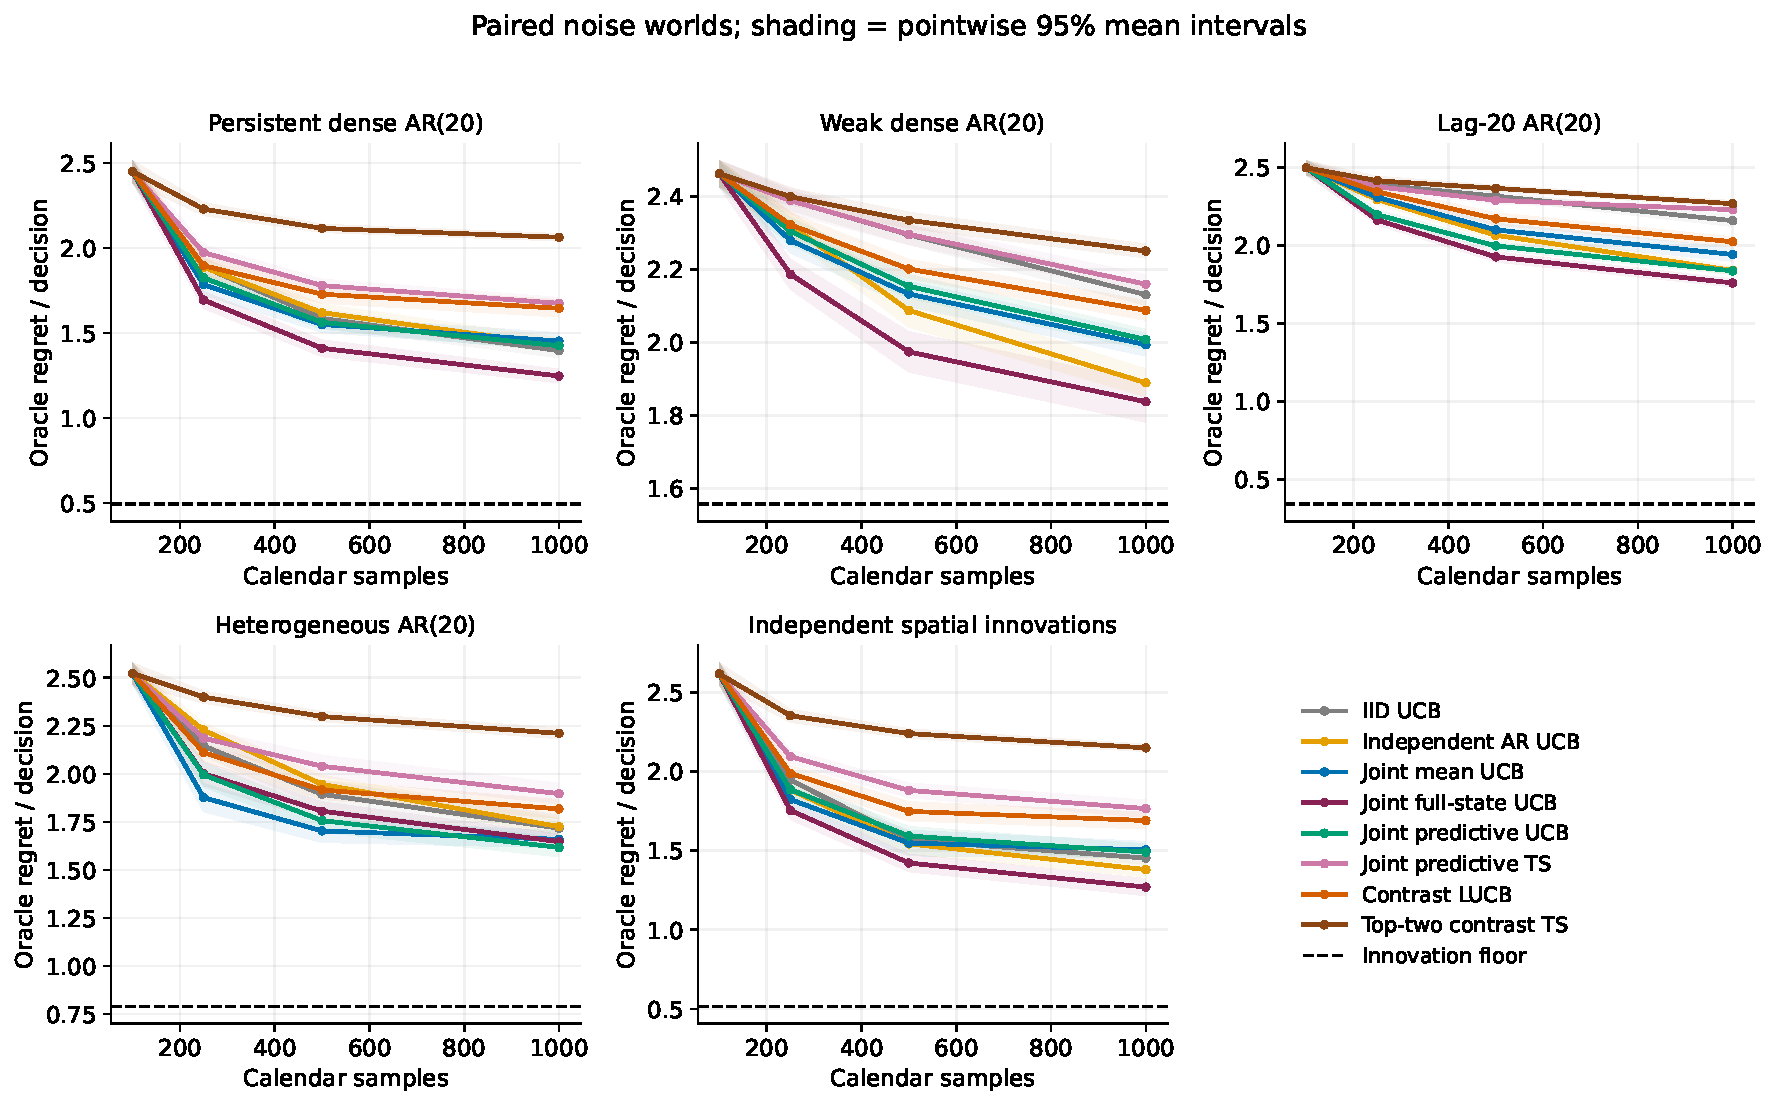
\includegraphics[width=\textwidth]{figures/spatiotemporal_bandits_oracle_regret.pdf}
\caption{Regret against the full-current-state oracle per decision. Dashed lines estimate the irreducible innovation coefficient. Shading gives pointwise 95\% intervals across independent worlds. The horizon includes 100 initial coverage observations.}
\label{spatiotemporal_bandits:fig:ar20-oracle}
\end{figure}
\begin{figure}[p]
\centering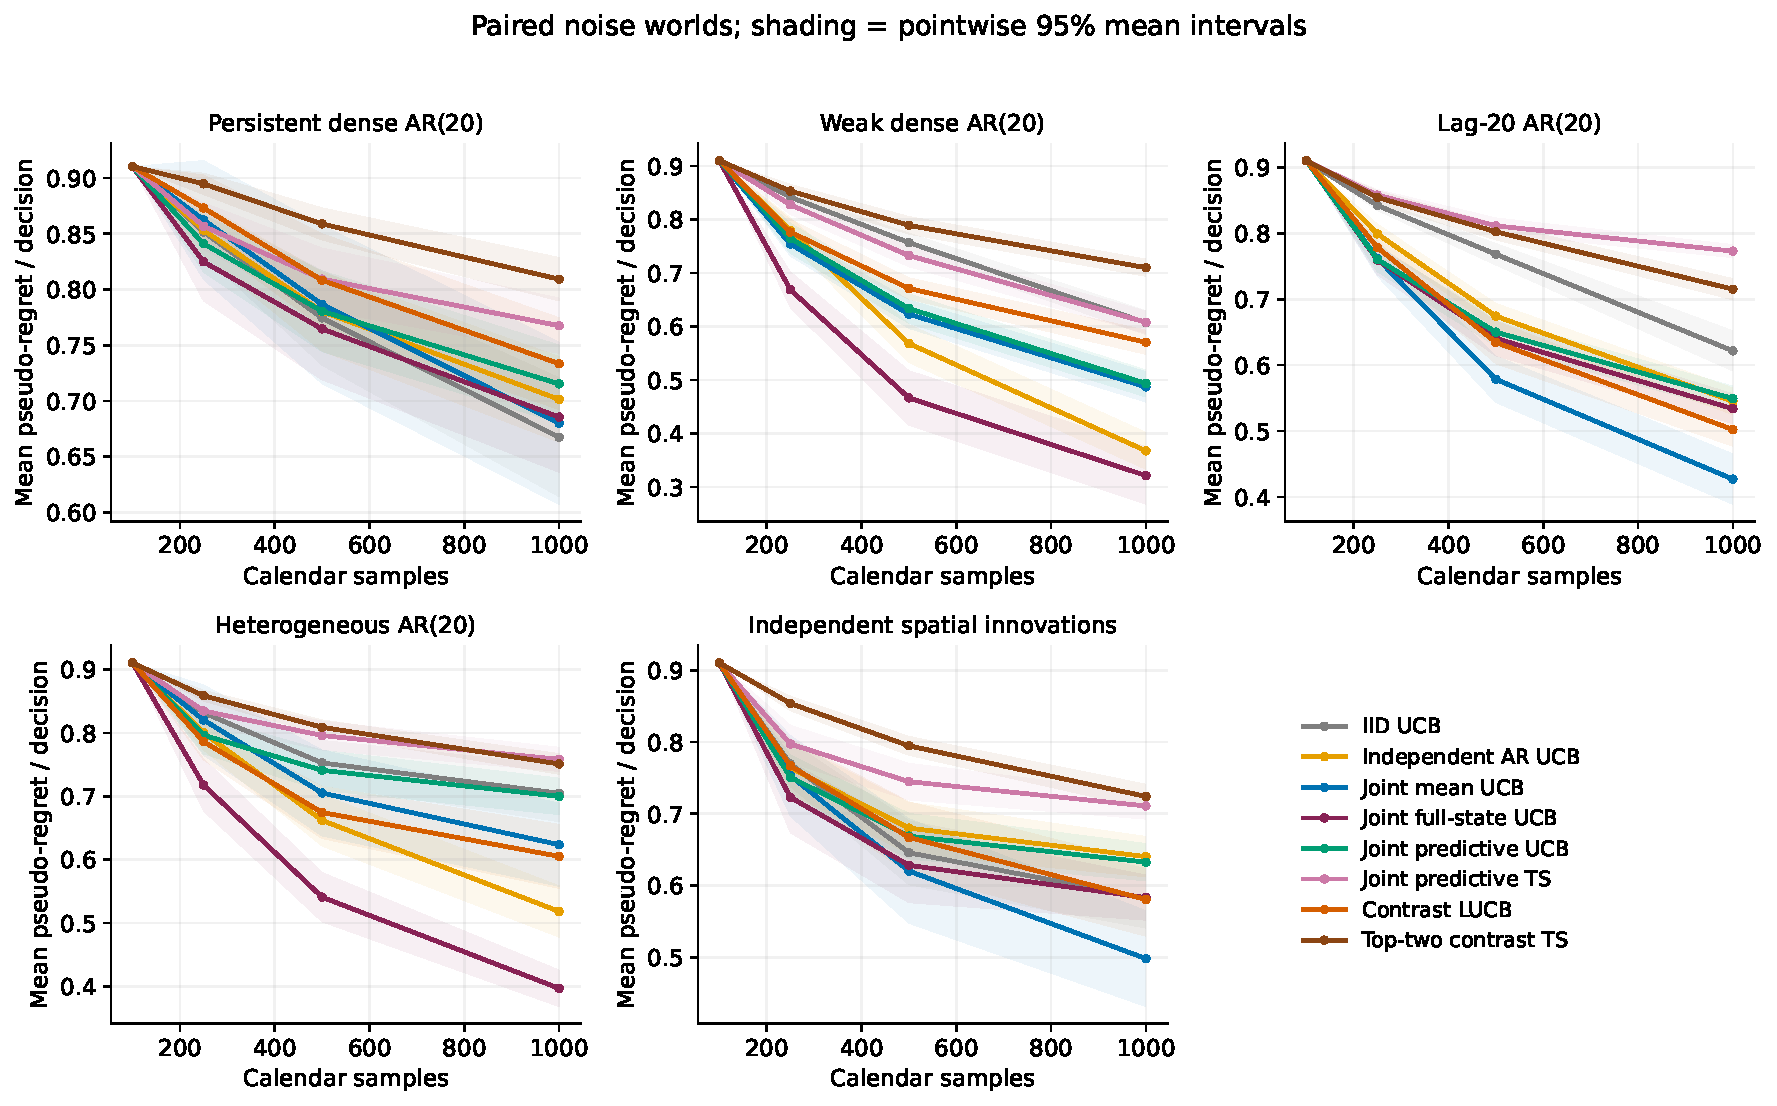
\includegraphics[width=\textwidth]{figures/spatiotemporal_bandits_mean_regret.pdf}
\caption{Permanent mean pseudo-regret per decision under the same paths. This comparator differs from both the current-state oracle and actual reward from the best permanent arm. Exploiting fluctuations can increase mean pseudo-regret while improving actual reward.}
\label{spatiotemporal_bandits:fig:ar20-mean}
\end{figure}
\begin{figure}[p]
\centering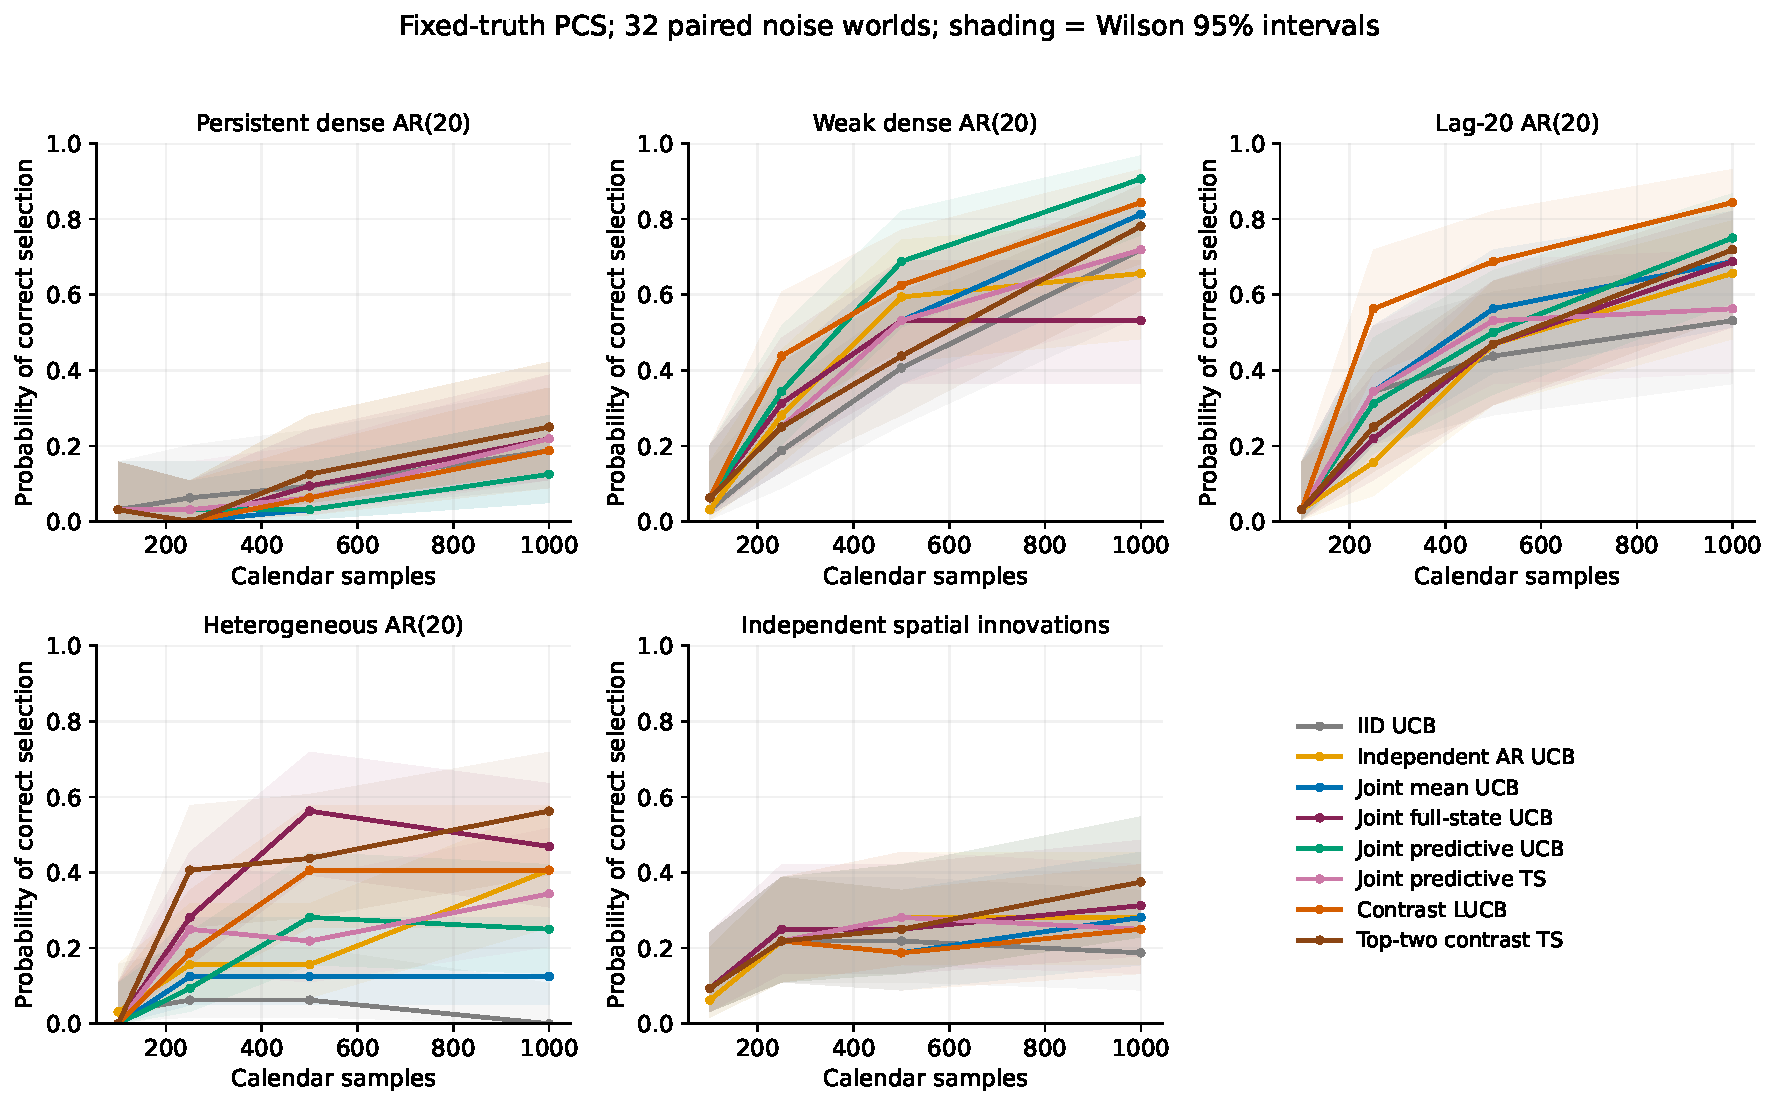
\includegraphics[width=\textwidth]{figures/spatiotemporal_bandits_pcs.pdf}
\caption{Fixed-truth PCS versus budget. Recommendations use permanent mean estimates. With 32 worlds, binomial uncertainty is substantial; Wilson intervals are reported in the CSV and findings. The fixed-budget decisions are not certified recommendations.}
\label{spatiotemporal_bandits:fig:ar20-pcs}
\end{figure}
\begin{figure}[p]
\centering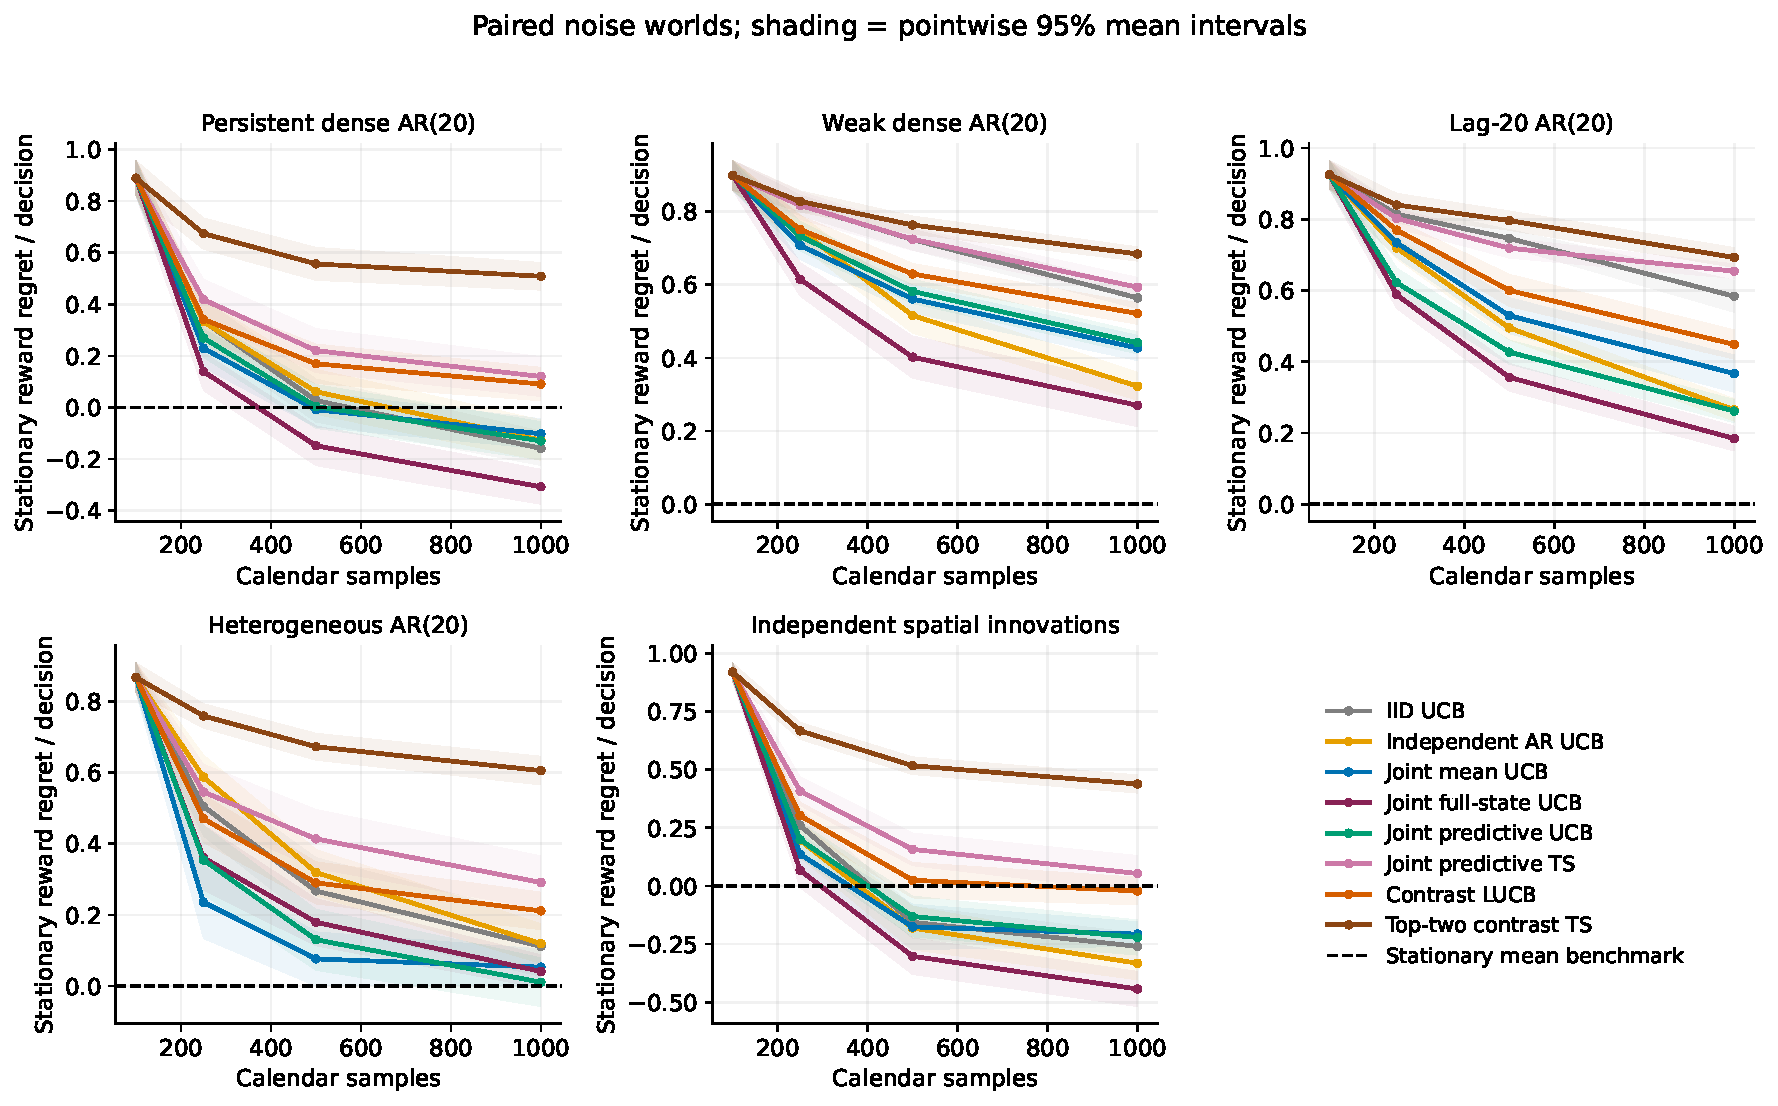
\includegraphics[width=\textwidth]{figures/spatiotemporal_bandits_stationary_reward_regret.pdf}
\caption{Actual reward regret against $T\mu_{b^*}$ per decision. Negative values mean the learner earns more than the stationary best mean by exploiting fluctuations. Its expectation equals reward regret against the fixed best-mean arm, but their finite-path realizations differ.}
\label{spatiotemporal_bandits:fig:ar20-stationary}
\end{figure}

The innovation-floor coefficients, estimated independently with 200,000 paired stationary Gaussian samples per configuration, are

Persistent $0.493$, Weak $1.556$, Lag 20 $0.340$, Heterogeneous $0.789$, Independent shocks $0.515$.


These are expectation bounds; a finite-world sampled regret need not exceed the estimated floor exactly. The full-past genie provides a separate path-simulation check. A declining finite-horizon regret ratio does not establish an asymptotic optimal coefficient.


For weak dependence, joint predictive UCB has PCS $0.906$, with Wilson interval $[0.758,0.968]$. The full-variance state UCB has smaller mean and oracle regret in this experiment. Selection accuracy and accumulated reward thus favor different decisions.

For lag-20 dependence, contrast LUCB gives PCS $0.844$ versus $0.281$ for round robin. The paired improvement is $0.562$ with approximate interval $[0.339,0.786]$. Joint mean UCB has smaller mean pseudo-regret, while full-state UCB has smaller oracle regret. The PCS-focused rule pays for comparison information rather than only extracting immediate reward.

For persistent dynamics, joint full-state UCB gives oracle regret $1.248$ per round versus $1.397$ for iid UCB. PCS remains poor, and joint mean UCB does not uniformly improve over iid UCB. Persistence helps state prediction while making permanent means harder to estimate. For a fully observed single arm, the long-run mean-noise scale is $q_i/(1-\sum_k a_{i,k})^2$; it is about 156 for the persistent profile. This full-observation scale illustrates the difficulty, without replacing the actual schedule-dependent likelihood.

For the same persistent state-UCB policy, mean pseudo-regret is $0.686$ per round, while actual reward regret against the stationary mean is $-0.308$ with interval $[-0.375,-0.240]$. The policy earns more than the best permanent mean by using predictable fluctuations, despite often choosing inferior permanent locations.

Removing fresh-innovation variance from Thompson draws improves oracle regret by 0.043--0.327 per round across these configurations. It does not uniformly improve the UCB rule. For homogeneous filters, adding a common positive variance inside a square root compresses differences between optimism bonuses; finite-budget performance also depends on exploration scale. These experiments compare fixed practical scales, not optimally tuned policy families.



The study validates computation and compares policies at one fixed mean surface. It does not establish general finite-budget optimality, robustness to incorrect graphs or unknown dynamics, or matching graph-dependent regret constants. The new implementation passes 642 assertions against dense likelihood and independent state calculations; large-model pilots exercise both 100-arm predictive policies. The analysis also checks paired-result completeness, nonnegative oracle/mean regret, and the pathwise identity $R_{\rm oracle}^{\pi}-R_{\rm oracle}^{b^*}=R_{\rm fixed}^{\pi}$.



\subsection{Discussion}
The physical model has fixed means, general autoregressive dynamics, and spatial correlation in the innovations. Graph regularization requires a separate deterministic restriction on permanent means. Shared traffic shocks alone do not imply similar permanent location quality.

Use the joint trajectory covariance, constrain or penalize graph differences, and retain smoothing bias in uncertainty statements. Joint lag-state filtering retains spatial information and delayed temporal prediction. General AR dependence replaces scalar freshness with a sequence of cross-arm impulse-response covariances.

The framework specializes established graph and linear Gaussian methods. Optimal allocation depends on evolving experiments and graph-constrained alternatives. A scalar sample-count allocation or automatic extension of a short-budget rule is insufficient. Unknown dynamics, innovation-graph uncertainty, measurement duration and costs, and attaining the information limits require further work.


\subsection{Reproduction and scope}
Use \path{experiments/graph_ar_mean.py} and the accompanying \path{results/general_ar/} directory. The superseded common-order-one paper, Bayesian mean-prior result, and experiments are preserved under \path{archive/common_ar1/} and \path{results/mean_selection/}; they do not establish the current fixed-mean higher-order claims.
\begin{verbatim}
python3 experiments/graph_ar_mean.py --verify
python3 experiments/graph_ar_mean.py --runs 200 --budget 60
python3 experiments/graph_ar_mean.py --render-only
.venv/bin/python -I experiments/spatiotemporal_policies.py --verify
.venv/bin/python -I experiments/spatiotemporal_policies.py \
  --runs 32 --horizon 1000 --jobs 4
.venv/bin/python -I experiments/spatiotemporal_policies_analysis.py
cd research/spatiotemporal_bandits
tectonic --only-cached --keep-logs manuscript.tex
\end{verbatim}
Exact confidence assumes known stable dynamics, positive definite Gaussian innovations, stationary initialization, and correct noise parameters. Mean bounds are supplied assumptions. The constrained-estimator helper covers positive definite information; the KKT statement also permits partially observed designs with an active positive multiplier. Gaussian deviations represent baseline-adjusted observations rather than literal negative traffic counts.


\clearpage
\section{Complete graph-alignment and resistance-design derivations}
\label{app:alignment}
The following results initially assume iid noise. Their graph information constants are not automatically a regret theorem for arbitrary restless sampling schedules.
\subsection{Introduction}
Consider a finite collection of stochastic alternatives with unknown mean rewards. A similarity graph can express prior information that two alternatives should perform similarly. An observation at one alternative can then inform estimates at another without directly observing its reward. The similarity selection index introduced by Sun, Li, and Fu~\cite{collected14}, and developed by Zhou, Fu, and Ryzhov~\cite{collected15}, formalizes this intuition through Laplacian smoothing. Their objective is final selection. The present question is how such information changes the cumulative regret of sequential decisions.

For classical stationary stochastic bandits, the principal targets are established. Worst-case expected regret for bounded rewards has optimal order $\sqrt{KT}$, and fixed-instance asymptotic lower bounds admit matching algorithms for important distribution families~\cite{collected20,collected21,collected22}. Consequently, a graph-based algorithm must be assessed against a restricted class of reward vectors that encodes what the graph tells the learner. A lower regret bound is possible because fewer alternative environments remain plausible, rather than because smoothing creates additional observations.

The phrase ``better alignment'' needs care. A graph can preserve the ordering of all means while providing no improvement in the information needed to distinguish them. Conversely, a graph may accurately identify several groups of nearly equivalent suboptimal alternatives, allowing a whole group to be rejected after a small pooled sample. Its usefulness depends on its geometry, the amount of reward variation allowed within it, and the gaps between groups. No scalar measure of visual resemblance or ranking agreement guarantees monotone regret improvement for arbitrary algorithms and graphs.

Our principal result shows why the full graph geometry matters. A complete graph with edge weights $1/m$ and a path with edge weights $(m-1)/2$ both have resistance diameter two. At homogeneous suboptimal means and supplied energy radius equal to the gap, every clique arm can independently become optimal within the model class. The path excludes these independent deviations: an average of its endpoints controls every interior mean. The clique requires an information coefficient proportional to $m$, while a concrete endpoint-based policy on the path has no linear dependence on $m$. This is a separation between graph-energy classes with identical diameter summaries, not a claim that spectral bandits or graph-aware exploration are new.

We develop the result in three steps. First, we express the information constant as an experimental design over least informative graph-energy alternatives. A finite-strength resolvent evaluates its inner optimization. Second, we show that the first-order cost of loosening alignment is governed by the minimum enclosing radius in the resistance embedding, equivalently an established maximum graph variance quantity. Third, a capped graph-design elimination algorithm uses this geometry and falls back to ordinary arm exploration on competitive components. We prove its regret bound, the achieved path separation, and a quantitative comparison under certified Laplacian perturbations. A simpler diameter-based pooling policy remains as a baseline and clarifies the connection to the original selection index.

The distinctions among results remain explicit. The information design gives the exact value of a lower-bound program for homogeneous components. The radius expansion describes that program's local sensitivity. The proposed policy achieves the path's improved arm-count dependence with conservative constants; it is not proved to attain the information constant for positive uncertainty. A separate standard lower-bound argument explains why unrestricted graph validation cannot preserve the reduced logarithmic constant for free.

\subsection{Related research and contribution boundary}
The original spectral selection index minimizes a squared estimation term plus a graph-Laplacian penalty~\cite{collected14}. Subsequent work develops sequential allocation for selecting the best alternative and permits updating similarity information~\cite{collected15}. Those allocation objectives differ from cumulative reward: a positive limiting sampling fraction assigned to a suboptimal arm produces linear cumulative regret. We retain the graph estimator's interpretation while changing the allocation objective.

Graph-smooth cumulative-regret bandits already appear in SpectralUCB and related algorithms~\cite{collected1,collected17}. They use graph spectral structure to reduce effective statistical complexity. We therefore do not claim that graph arms, Laplacian regularization, or a spectral confidence index constitute a new problem or algorithmic principle.

Clustered bandits are also established. Carlsson, Dubhashi, and Johansson~\cite{collected18} analyze hierarchical Thompson sampling and show how clustering quality affects regret under dominance assumptions. Gore and Chaporkar's Clus-UCB preprint~\cite{collected19} directly studies known clusters with bounded mean differences, derives an information lower bound, and proposes an index that shares observations within clusters. This is a close comparator for our pooling analysis. The preprint is cited as such; no publication status is assumed.

Our lower-bound starting point is the structured-bandit change-of-measure program of Combes, Magureanu, and Proutiere~\cite{collected11}. The maximum graph variance construction underlying our resistance design is established by Devriendt, Martin-Gutierrez, and Lambiotte~\cite{collected24}. Graph-aware pure exploration and resistance-based influence measures also appear in GRUB~\cite{collected2}. We do not claim to introduce experimental design, resistance geometry, or eliminating unsampled graph arms. The candidate contributions are the graph-energy information sensitivity, its explicit separation from diameter compression, and the accompanying cumulative-regret analysis and certified perturbation comparison.

The clique formula needs particularly careful positioning. For homogeneous clusters, Clus-UCB's information expression has the form $m\Gamma/[d+(m-1)b]$. Substituting Gaussian divergences gives the same algebraic shape as our clique constant with effective width $S/\sqrt{w(m-1)}$. This is our comparison, not a Gaussian theorem proved in that Bernoulli paper. It motivates making the general-graph separation, rather than the clique interpolation, the central result. We inspected Clus-UCB v2, including its discussion of incorrect widths~\cite{collected19}.

Model misspecification and unknown error are established topics in kernelized bandits~\cite{collected25}. Gap-adjusted approximation error~\cite{collected26} and graph-specific residual and eigenspace perturbation bounds~\cite{collected27} further constrain broad novelty claims. Our perturbation result assumes a certified comparison to a reference graph. We do not claim to learn that comparison from unrestricted selected-arm feedback. Independent mathematical review and a broader literature comparison remain necessary before asserting publication priority.

Similarity graphs must also be distinguished from feedback graphs. In our setting, a pull reveals only one reward. An edge restricts the possible means; it does not supply observations of adjacent arms. Observation noise is independent in the experiments. Dependence of the unknown means through a model class is sufficient for information sharing.

\subsection{Model and definitions of alignment}
\subsubsection{Bandit observations}
There are $K$ arms. At time $t$, an adapted policy selects $A_t$ and observes
\begin{equation}
 Y_t=\mu_{A_t}+\xi_t,\qquad \mu\in[0,1]^K.
 \label{alignment_paper:eq:model}
\end{equation}
Conditional on the past and the chosen arm, the noise has zero mean and satisfies
$\E[\exp(u\xi_t)\mid\mathcal F_{t-1},A_t]\le\exp(u^2\sigma^2/2)$ for every $u\in\R$.
Independent iid arm streams with common known sub-Gaussian proxy $\sigma$ suffice. Our lower bounds specialize to independent $N(\mu_i,\sigma^2)$ rewards with known variance. Define
\begin{equation}
 \mu^\star=\max_i\mu_i,\quad \Delta_i=\mu^\star-\mu_i,
 \quad \mathcal R_T=\sum_{t=1}^T\Delta_{A_t},\quad
 R_T=\E[\mathcal R_T].
\end{equation}
All regret is measured with the original means, even when the selection index is smoothed.

\subsubsection{Ordinal alignment}
Let $W$ be symmetric with nonnegative off-diagonal weights, write $\one$ for the all-ones vector, and let
$L=\diag(W\one)-W$. Write
\begin{equation}
 Q_\lambda=(I+\lambda L)^{-1},\qquad z_\lambda=Q_\lambda\bar Y.
 \label{alignment_paper:eq:sindex}
\end{equation}
We call a filter ordinally aligned at $\mu$ when $Q_\lambda\mu$ preserves its strict reward comparisons. This describes the order-preservation property relevant here. It does not replace the specific structural definitions of an aligned graph used in the earlier selection literature. In particular, the original WSC definition includes equal-degree and reward-distance conditions, while the later dissertation relaxes the structural condition~\cite{collected14,collected16}.

\begin{proposition}[Order preservation need not improve a comparison]
For the complete graph with common edge weight $w>0$,
\begin{equation}
 Q_\lambda=qI+(1-q)\frac{\one\one^\top}{K},\qquad
 q=(1+\lambda wK)^{-1}.
\end{equation}
For every vector $y$, $z_i-z_j=q(y_i-y_j)$. Thus the smoothed and raw sample means select exactly the same maximizer. With independent Gaussian sample means based on equal fixed counts $n$, both the true pairwise gap and its standard deviation are multiplied by $q$, leaving the signal-to-noise ratio unchanged.
\label{alignment_paper:prop:ordinal}
\end{proposition}
\begin{proof}
The complete-graph Laplacian is $w(KI-\one\one^\top)$. Its eigenvalue is zero on constants and $wK$ on their orthogonal complement. Inverting on these two subspaces gives the displayed expression. Pairwise differences remove the common-average term. Their raw variance is $2\sigma^2/n$, and their filtered variance is $q^2 2\sigma^2/n$.
\end{proof}
This example shows the limitation of rank preservation as a performance claim. It does not claim that every algorithm using a complete graph behaves identically to UCB.

\subsubsection{Quantitative alignment through graph energy}
Choose a fixed partition $\mathcal P=\{C_1,\ldots,C_M\}$ of the arms. A graph may already have these connected components, or a partition may be constructed and cross-partition edges removed. Let $L_c$ denote the resulting connected component Laplacian; singletons are permitted. Removing edges is part of the model construction, not an assumption that a connected original graph has zero cross edges.

The learner is supplied with valid local certificates
\begin{equation}
 \mu_c^\top L_c\mu_c\le S_c^2.
 \label{alignment_paper:eq:energy}
\end{equation}
The corresponding model class is
\begin{equation}
 \mathcal M_{\mathcal P,L,S}=\{\nu\in[0,1]^K:
       \nu_c^\top L_c\nu_c\le S_c^2\ \text{for all }c\}.
 \label{alignment_paper:eq:class}
\end{equation}
The certificates are prior information available to the policy. Their true values cannot silently be computed from unknown rewards during a real deployment.

For a connected component, define effective resistance
$r_{ij}^{\rm eff}=(e_i-e_j)^\top L_c^\dagger(e_i-e_j)$ and resistance diameter
$D_c^{\rm eff}=\max_{i,j\in C_c}r_{ij}^{\rm eff}$. Use $D_c^{\rm eff}=0$ for a singleton.

\begin{lemma}[Energy certifies reward diameter]
If \eqref{alignment_paper:eq:energy} holds, then
\begin{equation}
 |\mu_i-\mu_j|\le S_c\sqrt{r_{ij}^{\rm eff}},\qquad
 \max_{i\in C_c}\mu_i-\min_{i\in C_c}\mu_i
 \le\varepsilon_c:=\min\{1,S_c\sqrt{D_c^{\rm eff}}\}.
 \label{alignment_paper:eq:width}
\end{equation}
\label{alignment_paper:lem:resistance}
\end{lemma}
\begin{proof}
The vector $e_i-e_j$ is orthogonal to constants. On this subspace, factor its inner product with $\mu_c$ through $L_c^{\dagger/2}$ and $L_c^{1/2}$. Cauchy--Schwarz gives
$|(e_i-e_j)^\top\mu_c|^2\le
((e_i-e_j)^\top L_c^\dagger(e_i-e_j))(\mu_c^\top L_c\mu_c)$.
Bounded means additionally give diameter at most one.
\end{proof}
The product $S_c\sqrt{D_c^{\rm eff}}$ is invariant to a common rescaling of all component weights, provided the energy certificate is rescaled consistently. Shrinking weights without changing the information they represent is therefore not a substantive improvement in alignment.

Let $v_c=\max_{i\in C_c}\mu_i$, $\Gamma_c=\mu^\star-v_c$, and
$\mathcal O=\{c:\Gamma_c=0\}$. The relevant dimensionless uncertainty for rejecting a suboptimal component is $\varepsilon_c/\Gamma_c$. Neither $\Gamma_c$ nor this ratio is an algorithm input.

\subsection{From the spectral index to a pooling policy}
\subsubsection{Count-weighted spectral pooling}
Let $n_i$ and $\bar Y_i$ denote observed counts and sample means. The count-weighted analogue of the selection index solves
\begin{equation}
 \widehat f_\lambda\in\argmin_f
       \sum_{i:n_i>0}n_i(f_i-\bar Y_i)^2+\lambda f^\top Lf,
 \label{alignment_paper:eq:weighted}
\end{equation}
where $L$ is the block-diagonal Laplacian of the chosen partition. After every component has an observation, the solution is unique: a vector in the null spaces of both $\diag(n_i)$ and $L$ must vanish on every component. As $\lambda\to\infty$, nonconstant component modes are suppressed. Minimizing the remaining squared-error objective over constants gives
\begin{equation}
 \widehat f_{\infty,i}=\widehat p_c
 =\frac{\sum_{s:A_s\in C_c}Y_s}{N_c},\qquad i\in C_c,
 \quad N_c=\sum_{i\in C_c}n_i.
 \label{alignment_paper:eq:pool}
\end{equation}
This is a spectral pooling limit. It weights observations by counts; it is not the unweighted average of available arm averages. For unequal counts it differs from applying a fixed $Q_\lambda$ to the raw means. We do not invoke the earlier order-preservation theorem for this modified estimator.

The conditional mean of the pooled observation sequence is the average of the actual means of the sampled arms. Because selection is adaptive, $\widehat p_c$ is not an iid estimate of a fixed component mean when its arms differ. The component diameter certificate controls this drift.

\subsubsection{Algorithm}
Assume horizon $T\ge M$ and confidence level $\delta\in(0,1)$. Put
\begin{equation}
 \ell=\log\frac{2(K+M)T}{\delta},\qquad
 b(n)=\sigma\sqrt{\frac{2\ell}{n}},\quad b(0)=+\infty.
 \label{alignment_paper:eq:radius}
\end{equation}
For an unsampled arm set $u_i=+\infty$; otherwise set
$u_i=\bar Y_i+b(n_i)$. Define
\begin{equation}
 i_c\in\argmax_{i\in C_c}u_i,\qquad
 U_c=\min\{u_{i_c},\widehat p_c+b(N_c)+\varepsilon_c\}.
 \label{alignment_paper:eq:index}
\end{equation}
The policy, called spectral pooling UCB (SP-UCB) in this draft, is:
\begin{enumerate}
 \item Pull one predetermined representative of each component.
 \item At subsequent rounds select $c_t\in\argmax_c U_c$.
 \item Pull $A_t=i_{c_t}$ and update its arm and component statistics.
\end{enumerate}
Tie breaking uses a fixed arm ordering. There is no all-arm initialization requirement: a clearly suboptimal component can be rejected before all its members are sampled. An uncertain optimal component retains ordinary arm exploration through $i_c$.

The minimum in \eqref{alignment_paper:eq:index} combines two valid bounds on the same target $v_c$. Its validity depends on the supplied certificate. Taking a minimum with an ordinary UCB is not protection against a false graph assertion.

\subsubsection{Confidence under adaptive pooling}
For the $n$th observation from component $c$, let $B_{c,n}$ be the average of the means of the $n$ arms actually pulled there, including repetitions. A uniform event $\mathcal E$ is
\begin{equation}
 |\bar Y_i-\mu_i|\le b(n_i),\qquad
 |\widehat p_c-B_{c,N_c}|\le b(N_c)
 \label{alignment_paper:eq:event}
\end{equation}
for all nonzero arm and component counts through $T$.

\begin{lemma}[Uniform confidence]
Under \eqref{alignment_paper:eq:model}, $\Prob(\mathcal E)\ge1-\delta$. On this event, every $U_c$ in \eqref{alignment_paper:eq:index} is an upper bound on $v_c$.
\label{alignment_paper:lem:confidence}
\end{lemma}
\begin{proof}
For a fixed arm or component, the selected-noise sum $Z_t$ and count $N_t$ give the exponential supermartingale
$\exp(uZ_t-u^2\sigma^2N_t/2)$. Stop it at the $n$th corresponding pull or at $T$. On the event that the $n$th pull occurs, the upper-tail probability for $Z\ge nb(n)$ is at most $e^{-\ell}$, using $u=b(n)/\sigma^2$. Apply the same argument to the lower tail. A union bound over $K+M$ processes and $n=1,\ldots,T$ gives failure probability at most $2(K+M)Te^{-\ell}=\delta$. This argument does not treat a stopped sample average as Gaussian.

For a component, $v_c-\varepsilon_c\le B_{c,N_c}\le v_c$. Thus $\widehat p_c+b(N_c)+\varepsilon_c\ge v_c$ on $\mathcal E$. The largest ordinary arm upper bound also exceeds $v_c$. Their minimum remains an upper bound.
\end{proof}

\subsubsection{Finite-time regret}
Define the ordinary component bound
\begin{equation}
 A_c=\sum_{i\in C_c:\Delta_i>0}
        \left(\Delta_i+\frac{8\sigma^2\ell}{\Delta_i}\right).
 \label{alignment_paper:eq:Ac}
\end{equation}
For suboptimal components define
\begin{equation}
 H_c=\begin{cases}
 (\Gamma_c+\varepsilon_c)
 \left(1+\dfrac{8\sigma^2\ell}{(\Gamma_c-\varepsilon_c)^2}\right),
       &\varepsilon_c<\Gamma_c,\\
 +\infty,&\varepsilon_c\ge\Gamma_c.
 \end{cases}
 \label{alignment_paper:eq:Hc}
\end{equation}

\begin{theorem}[Alignment-sensitive finite-time guarantee]
If the graph-derived or directly supplied diameter certificates are valid, SP-UCB satisfies, on $\mathcal E$,
\begin{equation}
 \mathcal R_T\le
     \sum_{c\in\mathcal O}A_c+
     \sum_{c\notin\mathcal O}\min\{A_c,H_c\}.
 \label{alignment_paper:eq:regret}
\end{equation}
Consequently, expected regret is at most the right side plus $\delta T$.
\label{alignment_paper:thm:upper}
\end{theorem}
\begin{proof}
At any post-initialization round selecting arm $i$ in component $c$, optimism of an optimal component gives
$\mu^\star\le U_c\le u_i\le\mu_i+2b(n_i)$ whenever $n_i>0$.
Thus a suboptimal arm can be selected with a positive pre-pull count only if
$n_i\le8\sigma^2\ell/\Delta_i^2$.
Its first pull, including a possible initialization pull, contributes the extra one. Therefore
$n_i(T)\le1+8\sigma^2\ell/\Delta_i^2$, yielding $A_c$.

The pooled index also gives
$\mu^\star\le U_c\le v_c+2b(N_c)+\varepsilon_c$.
If $\Gamma_c>\varepsilon_c$, a component can be selected only with
$N_c\le8\sigma^2\ell/(\Gamma_c-\varepsilon_c)^2$ beforehand, except for its first initialization pull. Hence
$N_c(T)\le1+8\sigma^2\ell/(\Gamma_c-\varepsilon_c)^2$.
Each such pull has regret at most $\Gamma_c+\varepsilon_c$, giving $H_c$.
Both bounds hold simultaneously, so take their minimum. On the failure event, bounded means give $\mathcal R_T\le T$.
\end{proof}

\begin{corollary}[Improved certificates tighten the component guarantee]
For a fixed partition and reward vector, $H_c$ is increasing in $\varepsilon_c$ on $[0,\Gamma_c)$. Thus tightening a valid certificate cannot worsen the bound in \eqref{alignment_paper:eq:regret}. If $\varepsilon_c=0$, every arm in that component has gap $\Gamma_c$, and the leading logarithmic terms of $A_c$ and $H_c$ differ by a factor $|C_c|$.
\end{corollary}
\begin{proof}
The derivative of $(\Gamma+\varepsilon)/(\Gamma-\varepsilon)^2$ is
$(3\Gamma+\varepsilon)/(\Gamma-\varepsilon)^3>0$; the nonlogarithmic term is increasing as well. At zero width, $A_c=|C_c|\Gamma_c+8\sigma^2\ell|C_c|/\Gamma_c$, whereas $H_c=\Gamma_c+8\sigma^2\ell/\Gamma_c$.
\end{proof}
This is monotonicity of a proved upper bound, not a pathwise ordering between two policies with different certificates. Changing the partition also changes component gaps and the number of components; no universal monotonicity assertion follows from reducing an empirical graph-error score.

\subsection{How alignment changes the information lower bound}
\subsubsection{General graph classes}
For this section assume Gaussian rewards with known common variance $\sigma^2$, a unique optimal arm $i^\star$, and $\mu^\star<1$. An algorithm is uniformly efficient on a class if its regret is $o(T^a)$ for every $a>0$ at every member of that class. Define confusing alternatives
\begin{equation}
 \mathcal B(\mu)=\{\nu\in\mathcal M_{\mathcal P,L,S}:
       \nu_{i^\star}=\mu^\star,\ \max_j\nu_j>\mu^\star\}.
\end{equation}
The established structured-bandit information principle~\cite{collected11} yields the program
\begin{align}
 C_{L,S}(\mu)=\inf_{x_i\ge0}\quad&\sum_{i\ne i^\star}x_i\Delta_i,\label{alignment_paper:eq:info}\\
 \text{subject to}\quad&
 \sum_{i\ne i^\star}x_i\frac{(\mu_i-\nu_i)^2}{2\sigma^2}\ge1
       \quad\text{for every }\nu\in\mathcal B(\mu).\nonumber
\end{align}
In particular,
\begin{equation}
 \liminf_{T\to\infty}\frac{R_T}{\log T}\ge C_{L,S}(\mu).
 \label{alignment_paper:eq:lower}
\end{equation}
The normalization $x_i$ represents the number of samples of arm $i$ per unit $\log T$. Alternatives agreeing on the optimal arm cannot be rejected by cost-free optimal-arm observations alone.

The following monotonicity is a property of the information available, independent of a particular algorithm. If two supplied classes contain the true vector and
$\mathcal M_1\subseteq\mathcal M_2$, then $C_{\mathcal M_1}(\mu)\le C_{\mathcal M_2}(\mu)$. The first class has fewer alternative constraints in \eqref{alignment_paper:eq:info}. Decreasing valid $S_c$ with $L_c$ fixed gives this nesting. Arbitrarily changing graph edges does not necessarily do so.

For completeness, the change-of-measure reasoning is as follows. Comparing $\mu$ with a confusing $\nu$, the KL divergence of histories is
$\sum_i\E_\mu[n_i(T)](\mu_i-\nu_i)^2/(2\sigma^2)$.
Consider the event that the original best arm is played at least $T/2$ times. Uniform efficiency makes its probability approach one under $\mu$ and at most $o(T^{-1+a})$ under $\nu$, for every $a>0$. The binary KL divergence of this event is consequently at least $(1-o(1))\log T$. This gives each information constraint; normalizing sample counts and passing to a finite convergent subsequence of any bounded-cost allocation gives \eqref{alignment_paper:eq:lower}. If normalized regret is unbounded, the inequality is immediate.


\subsubsection{A graph-specific information design}
The diameter bound \eqref{alignment_paper:eq:width} can discard statistically useful geometry. Consider a homogeneous suboptimal component with connected Laplacian $L$, $m\ge2$ arms of true mean $a$, gap $\Gamma=\mu^\star-a$, and supplied energy budget $S^2$. Let $s=S/\Gamma$ and let $\mathscr P_m=\{p\ge0:\one^\top p=1\}$. Define
\begin{align}
 F_L(p,s)&=\min_{i\in\{1,\ldots,m\}}\ \min_{z\in\mathcal Z_i(s)}
                 \sum_jp_jz_j^2,\label{alignment_paper:eq:designF}\\
 \mathcal Z_i(s)&=\{z\in[0,1]^m:z_i=1,\ z^\top Lz\le s^2\},\qquad
 F_L^\star(s)=\max_{p\in\mathscr P_m}F_L(p,s).\nonumber
\end{align}
Here $p$ allocates observations, rather than graph edge weights. The least informative alternative $z$ describes a displacement from the true constant vector, normalized by the gap.

\begin{theorem}[Exact information design for a homogeneous graph component]
When the optimal component is a singleton and all other true components are homogeneous, the program \eqref{alignment_paper:eq:info} separates into component contributions
\begin{equation}
 C_{L,S,c}(\mu)=\frac{2\sigma^2}{\Gamma_c F_{L_c}^\star(S_c/\Gamma_c)}.
 \label{alignment_paper:eq:generaldesignconstant}
\end{equation}
For a fixed graph, $F_L^\star$ is nonincreasing in $s$, lies in $[1/m,1]$, and equals one at $s=0$. For a fixed $s$, $F_L(p,s)$ is concave and continuous in $p$.
\label{alignment_paper:thm:generaldesign}
\end{theorem}
\begin{proof}
Write a component allocation as $x=Xp$, where $X=\sum_jx_j$. Clipping any alternative's displacements to $[0,\Gamma]$ decreases both their squared information cost and graph energy, because clipping is a contraction on every edge. Scaling a displacement that exceeds $\Gamma$ gives a boundary alternative with one coordinate equal to $\Gamma$. Conversely, adding a common arbitrarily small positive displacement to a boundary alternative makes it strictly confusing without changing energy; $\mu^\star<1$ keeps it inside the mean domain. The infimal information rate is therefore $X\Gamma^2F_L(p,s)/(2\sigma^2)$. Minimizing the regret cost $X\Gamma$ proves \eqref{alignment_paper:eq:generaldesignconstant}. Changes in other components cannot make this alternative harder to distinguish, so component costs add.

The sets $\mathcal Z_i(s)$ are compact and nonempty, containing $\one$. Each candidate objective is linear in $p$, which gives concavity and continuity of their minimum. Increasing $s$ expands the candidate sets. For uniform $p$, $z_i=1$ implies objective at least $1/m$, while $\one$ gives the upper bound one for every $p$. At zero energy, connectedness forces $z=\one$.
\end{proof}
This theorem evaluates the established information framework~\cite{collected11}; it does not claim that an arbitrary maximizer of \eqref{alignment_paper:eq:designF} immediately gives an implementable asymptotically optimal bandit policy.

\begin{lemma}[Resolvent oracle for the least informative alternative]
For $p_j>0$ and $s>0$, with $D_p=\diag(p)$, the inner minimum in \eqref{alignment_paper:eq:designF} equals
\begin{equation}
 \sup_{\tau\ge0}\left\{
 \frac{1}{[(D_p+\tau L)^{-1}]_{ii}}-\tau s^2\right\}.
 \label{alignment_paper:eq:resolventoracle}
\end{equation}
For a fixed multiplier, its minimizing vector is
$z=(D_p+\tau L)^{-1}e_i/[(D_p+\tau L)^{-1}]_{ii}$.
\label{alignment_paper:lem:resolvent}
\end{lemma}
\begin{proof}
Relax the box constraint temporarily and dualize the energy inequality. Minimizing $z^\top(D_p+\tau L)z$ subject to $z_i=1$ gives the displayed inverse formula by a Lagrange multiplier. The free-coordinate equations and the maximum principle imply $0\le z_j\le1$, so removing the box constraint does not alter this minimum. The constant vector is strictly feasible for the energy inequality when $s>0$, giving strong convex duality. For $s=0$ the value follows by the limit $\tau\to\infty$. Designs with zero entries are handled by limits of positive designs, using continuity in $p$.
\end{proof}
With uniform design, $(D_p+\tau L)^{-1}=m(I+m\tau L)^{-1}$. Thus the finite-strength spectral resolvent used in the selection index also appears in an exact information calculation, not just in the infinite-smoothing pooling limit. This is a variational connection, not a regret guarantee for selecting the largest fixed-strength index.

\subsubsection{Resistance geometry determines local alignment sensitivity}
Let $\mathcal D$ be the matrix of pairwise effective resistances. For a design $p$, define
\begin{equation}
 \kappa_L(p)=\max_i\sqrt{(e_i-p)^\top L^\dagger(e_i-p)},\qquad
 \rho_L=\min_{p\in\mathscr P_m}\kappa_L(p).
 \label{alignment_paper:eq:radiusdesign}
\end{equation}
The vectors $v_i=L^{\dagger/2}e_i$ embed the arms into Euclidean space with squared distances $\|v_i-v_j\|^2=\mathcal D_{ij}$. The quantity $\rho_L$ is the radius of their smallest enclosing ball. Its center lies in their convex hull, so it has a probability-vector representation. This geometry and the equivalent maximum graph variance problem are established~\cite{collected24}; the next theorem uses them to quantify bandit information sensitivity.

\begin{lemma}[Computable resistance design and a stopping certificate]
\begin{equation}
 \rho_L^2=\max_{p\in\mathscr P_m}\frac12p^\top\mathcal Dp.
 \label{alignment_paper:eq:maxvariance}
\end{equation}
For every $p$, $V(p)=p^\top\mathcal Dp/2$ is a lower bound on $\rho_L^2$, and $\kappa_L(p)^2$ is an upper bound, with gap
\begin{equation}
 \kappa_L(p)^2-V(p)=\max_i(\mathcal Dp)_i-p^\top\mathcal Dp.
 \label{alignment_paper:eq:designgap}
\end{equation}
\label{alignment_paper:lem:designradius}
\end{lemma}
\begin{proof}
For any center $v(p)$, the squared distance to arm $i$ is
$(\mathcal Dp)_i-V(p)$. The variance of any distribution $q$ about its own mean is $V(q)$; its average squared distance about any other center is $V(q)+\|v(q)-v(p)\|^2$. Consequently every enclosing ball has squared radius at least $\max_qV(q)$. At a maximum-variance distribution $p^\star$, simplex optimality gives $(\mathcal Dp^\star)_i\le(p^\star)^\top\mathcal Dp^\star$ for every $i$, with equality on its support. Its center therefore has maximum squared distance $V(p^\star)$, proving equality. Substituting the distance formula gives the gap certificate.
\end{proof}
The radius is invariant in the relevant units: rescaling $L$ by $b>0$ changes $\rho_L$ by $b^{-1/2}$ and a consistently scaled $S$ by $b^{1/2}$. A numerical design need not achieve exact optimality; its computed upper radius gives a valid, possibly looser, certificate.

\begin{theorem}[First-order graph alignment sensitivity]
Let $D=\max_{i,j}\mathcal D_{ij}$. For $s\sqrt D\le1$,
\begin{equation}
 1-2s\rho_L\ \le F_L^\star(s)
 \le 1-2s\rho_L+s^2D.
 \label{alignment_paper:eq:firstorderF}
\end{equation}
For every $s\ge0$,
\begin{equation}
 F_L^\star(s)\ge(1-s\rho_L)_+^2.
 \label{alignment_paper:eq:jensenF}
\end{equation}
In particular, as $S/\Gamma\downarrow0$,
\begin{equation}
 \frac{C_{L,S,c}(\mu)}{2\sigma^2/\Gamma}
 =1+2\frac S\Gamma\rho_L
   +O\!\left(\frac{S^2}{\Gamma^2}D\right).
 \label{alignment_paper:eq:sensitivity}
\end{equation}
\label{alignment_paper:thm:sensitivity}
\end{theorem}
\begin{proof}
For $z\in\mathcal Z_i(s)$, energy Cauchy--Schwarz gives
$1-p^\top z\le s\sqrt{(e_i-p)^\top L^\dagger(e_i-p)}$.
Jensen's inequality and nonnegativity then give
$\sum_jp_jz_j^2\ge(1-s\kappa_L(p))_+^2$. Optimize over $p$ for \eqref{alignment_paper:eq:jensenF}.

For the sharper expansion, write $z=\one-su$ with $u_i=0$ and $u^\top Lu\le1$. The largest possible $p^\top u$ is $\kappa_i(p)=\sqrt{(e_i-p)^\top L^\dagger(e_i-p)}$. A maximizer is obtained from the inverse grounded Laplacian applied to $p_{-i}$ and normalized to unit energy. Its coordinates are nonnegative by the maximum principle. Energy Cauchy--Schwarz additionally gives $u_j\le\sqrt{\mathcal D_{ij}}\le\sqrt D$, so $z$ is box-feasible when $s\sqrt D\le1$. The objective equals $1-2sp^\top u+s^2\sum_jp_ju_j^2$. Its nonnegative final term gives the lower bound $1-2s\kappa_L(p)$; taking a maximizing $u$ for an arm attaining $\kappa_L(p)$ gives the upper bound $1-2s\kappa_L(p)+s^2D$. Optimize over $p$. The information expansion follows by inversion for sufficiently small $s$, using $\rho_L^2\le D$.
\end{proof}
The leading sensitivity is therefore a graph-wide resistance radius, not the resistance diameter or the number of arms alone. A design minimizing that radius is first-order optimal for this information calculation. No first-order optimality claim is made for the regret constant of the algorithm introduced below.

\subsubsection{Certified graph perturbations}
\begin{proposition}[An explicit price for a certified Laplacian error]
Suppose, on the subspace orthogonal to constants,
\begin{equation}
 (1-\eta)L\preceq\widehat L\preceq(1+\eta)L,\qquad 0\le\eta<1.
 \label{alignment_paper:eq:lapperturb}
\end{equation}
If $S$ is valid for $L$, then $\widehat S=\sqrt{1+\eta}\,S$ is valid for $\widehat L$, and
\begin{equation}
 \widehat S\rho_{\widehat L}
 \le S\rho_L\sqrt{\frac{1+\eta}{1-\eta}}.
 \label{alignment_paper:eq:perturbradius}
\end{equation}
The corresponding homogeneous-component information constants obey
\begin{equation}
 C_{L,S,c}\le C_{\widehat L,\widehat S,c}
 \le C_{L,\,S\sqrt{(1+\eta)/(1-\eta)},c}.
 \label{alignment_paper:eq:perturbinfo}
\end{equation}
\label{alignment_paper:prop:perturb}
\end{proposition}
\begin{proof}
The upper Loewner inequality certifies the true energy. Inverting the inequalities on the constant-free subspace bounds every resistance quadratic form between factors $(1+\eta)^{-1}$ and $(1-\eta)^{-1}$ of the original form. Minimize their maximum over designs to obtain \eqref{alignment_paper:eq:perturbradius}. The original energy ball of radius $S$ is contained in the estimated-graph energy ball of radius $\widehat S$, which in turn is contained in the original ball of radius $S\sqrt{(1+\eta)/(1-\eta)}$. Apply information monotonicity.
\end{proof}
For Laplacians with the same constant null space, an operator error bound
$\|\widehat L-L\|_{\rm op}\le\eta\lambda_2(L)$ suffices for \eqref{alignment_paper:eq:lapperturb}. This connects a certified graph error to both an algorithmic bias radius and an information-class comparison. The true reference graph and error bound are additional information; they are not assumed obtainable for free from bandit observations. Related spectral perturbation and mismatch questions already arise in graph-contextual bandits~\cite{collected27}.

\subsubsection{Graphs with identical diameters can have different exploration costs}
Compare two components with the same number $m\ge3$ of arms:
\begin{enumerate}
 \item A complete graph with edge weight $1/m$ has $\mathcal D_{ij}=2$ for distinct arms and $\rho_L^2=(m-1)/m$, attained by the uniform design.
 \item A path with edge weight $(m-1)/2$ has $\mathcal D_{ij}=2|i-j|/(m-1)$ and $\rho_L^2=1/2$, attained by placing half the design mass at each endpoint.
\end{enumerate}
For the path, an embedding with orthogonal successive increments has all its vertices at squared distance $1/2$ from the endpoint midpoint. The endpoints are squared distance two apart, so no smaller ball can enclose them. For the clique, the regular simplex has radius squared $(m-1)/m$. Both graphs have resistance diameter two.

\begin{corollary}[Diameter compression loses an unbounded information factor]
At a homogeneous instance with supplied $S=\Gamma$, the clique contribution is the unstructured value
\begin{equation}
 C_{\rm clique}=\frac{2\sigma^2m}{\Gamma},
 \label{alignment_paper:eq:cliqueseparation}
\end{equation}
whereas the path contribution satisfies
\begin{equation}
 C_{\rm path}\le
 \frac{2\sigma^2}{\Gamma(1-1/\sqrt2)^2}.
 \label{alignment_paper:eq:pathinformation}
\end{equation}
Their ratio is at least $m(1-1/\sqrt2)^2$, which grows without bound with $m$. The number of arms, true means, supplied energy budget, and resistance diameter are identical.
\label{alignment_paper:cor:informationseparation}
\end{corollary}
\begin{proof}
In the clique, a single-coordinate displacement of $\Gamma$ costs energy $\Gamma^2(m-1)/m< S^2$. Every arm can therefore independently become optimal, requiring its classical information allocation. For the path, use \eqref{alignment_paper:eq:jensenF} with $s=1$ and $\rho_L=1/\sqrt2$.
\end{proof}
This separation concerns the graph-energy classes, not superiority over all existing spectral algorithms. A bound based solely on $S\sqrt D$ gives the same width $\sqrt2\Gamma$ for both graphs and cannot express it. Nor do the normalized paths and cliques have identical Laplacian spectra: the example isolates the information lost by diameter compression.

\begin{figure}[t]
\centering
\begin{tikzpicture}
\begin{axis}[width=.9\linewidth,height=6cm,ymode=log,
 xlabel={Normalized supplied energy radius $S/\Gamma$},
 ylabel={Information constant divided by $2\sigma^2/\Gamma$},
 grid=major,legend columns=2,legend style={font=\small,at={(0.5,1.03)},anchor=south},xmin=0,xmax=1.3]
\addplot[red,thick] table[x=s,y=clique_constant_ratio,col sep=comma]{evidence/alignment_paper/results/geometry/information.csv};
\addlegendentry{Clique: exact information value}
\addplot[blue,thick,dashed] table[x=s,y=path_constant_upper,col sep=comma]{evidence/alignment_paper/results/geometry/information.csv};
\addlegendentry{Path: information upper bound}
\addplot[black,dotted,thick] table[x=s,y=classical_ratio,col sep=comma]{evidence/alignment_paper/results/geometry/information.csv};
\addlegendentry{Unstructured value}
\end{axis}
\end{tikzpicture}
\caption{Analytical information comparison at $m=256$. The path curve is $\min\{m,(1-s/\sqrt2)^{-2}\}$ and bounds the information-program value from above; it is not an attained policy coefficient or an exact path expression. At $s=1$ the clique value is $256$, while the path value is at most $11.66$.}
\label{alignment_paper:fig:geometryinformation}
\end{figure}



\subsubsection{A closed-form answer for homogeneous cliques}
The general program is difficult. The following solvable graph family gives a quantitative answer to the motivating question. The optimal component is a singleton. Each other component $c$ is a clique of $m_c\ge2$ arms, with common edge weight $w_c>0$. At the true instance its arms all have mean $a_c<\mu^\star$, so $\Gamma_c=\mu^\star-a_c$. Alternatives satisfy the energy certificate $S_c$ but need not be homogeneous. Define
\begin{equation}
 q_c=\frac{S_c}{\Gamma_c\sqrt{w_c(m_c-1)}},\qquad
 g_c=1+(m_c-1)\pos{1-q_c}^2.
 \label{alignment_paper:eq:alignmentratio}
\end{equation}

\begin{theorem}[Clique information constant]
For the graph-energy class just described, the value of \eqref{alignment_paper:eq:info} is
\begin{equation}
 C_{L,S}(\mu)=\sum_{c\ne c^\star}
 \frac{2\sigma^2 m_c\Gamma_c}
 {\Gamma_c^2+(m_c-1)
       \pos{\Gamma_c-S_c/\sqrt{w_c(m_c-1)}}^2}
 =\sum_{c\ne c^\star}\frac{2\sigma^2m_c}{\Gamma_c g_c}.
 \label{alignment_paper:eq:cliqueconstant}
\end{equation}
Thus $g_c$ is the reduction factor relative to that component's unstructured Gaussian information constant $2\sigma^2m_c/\Gamma_c$.
\label{alignment_paper:thm:clique}
\end{theorem}
\begin{proof}
Constraints separate by suboptimal component: alternatives raising a single component must be rejected, and any alternative raising multiple components contains at least one such information requirement. The true means, graph, and regret coefficients in a component are invariant to permutations of its arms. Averaging any feasible allocation over permutations preserves feasibility and cost, because each information constraint is linear in the allocation and the full alternative set is invariant. Hence an optimal component allocation can be uniform, $x_i=X/m$.

Fix an arm that an alternative raises above $\mu^\star$. At the infimum it is raised to $\mu^\star$, a movement $\Gamma$. The boundary is sufficient: scaling a nonnegative displacement toward the true constant vector reduces both its information cost and its graph energy. Displacements can first be clipped to $[0,\Gamma]$, which does not increase energy or squared distance. By convexity and symmetry, the other $m-1$ movements may be equal to $h$. The energy constraint is then
\begin{equation}
 w(m-1)(\Gamma-h)^2\le S^2,
\end{equation}
and the smallest squared distance occurs at
$h=\pos{\Gamma-S/\sqrt{w(m-1)}}$.
The infimal information per unit total allocation is
$[\Gamma^2+(m-1)h^2]/(2\sigma^2m)$.
Strictly improving alternatives approach this boundary continuously; when $S=0$, raise every arm in the component by the same amount instead. Since $\mu^\star<1$, the approximating alternatives remain in the mean domain. The smallest feasible $X$ is the reciprocal of this information rate. Multiplying by the common regret coefficient $\Gamma$ proves the result.
\end{proof}

At $q_c=0$, $g_c=m_c$ and the information cost becomes $2\sigma^2/\Gamma_c$: the clique behaves like one arm. For $q_c>1$, an individual arm can plausibly exceed the optimum while its peers retain their true means. At $q_c=1$ the same information constant follows by a limiting alternative with arbitrarily small peer changes. Thus $g_c=1$ for $q_c\ge1$, and the unstructured constant returns. The transition is continuous and depends on uncertainty relative to the reward gap.

For $m=8$, values $q=0,0.25,0.5,0.75,1$ give factors $8,4.9375,2.75,1.4375,1$. These are ratios of information lower-bound constants. They are not asserted finite-horizon speedups of SP-UCB.

The actual graph energy at the homogeneous true instance is zero even when a positive $S_c$ is supplied. In this theorem, $S_c$ measures how much mismatch the learner must allow, not the observed graph error. A true graph and a graph with a trustworthy tight certificate convey different amounts of information than the same graph with no certified relationship to rewards.

For a clique, Lemma~\ref{alignment_paper:lem:resistance} gives
\begin{equation}
 \varepsilon_c\le S_c\sqrt{\frac{2}{w_cm_c}}
 =\Gamma_c q_c\sqrt{\frac{2(m_c-1)}{m_c}},
 \label{alignment_paper:eq:cliquewidth}
\end{equation}
before clipping at one. Combining this with Theorem~\ref{alignment_paper:thm:upper} yields an explicit attainable upper bound in a strong-alignment regime. The information expression remains finite near $q_c=1$, whereas the pooled-only bound can become loose; its intersection with $A_c$ retains the classical guarantee. The different constants and thresholds expose the gap between the simple policy and an information-optimal allocation.



\subsubsection{The exact-alignment endpoint is achievable}
If every $S_c=0$, connectedness forces a constant mean on each component. Selecting any representative reduces the problem to an ordinary $M$-armed bandit. In the Gaussian case with a unique best component, a classical asymptotically optimal algorithm on these representatives achieves
\begin{equation}
 R_T=\left(\sum_{c\ne c^\star}\frac{2\sigma^2}{\Gamma_c}\right)\log T
      +o(\log T).
 \label{alignment_paper:eq:exact}
\end{equation}
The corresponding change-of-measure lower bound shifts all arms in a component together, and matches this expression. The reduction is thus attainable, independently of SP-UCB's conservative confidence constants. For bounded reward classes with $2\le M\le T$, the exact-component minimax rate is $\Theta(\sqrt{MT})$: a representative-based minimax policy supplies the upper bound, and a Bernoulli subclass with arbitrary component means supplies the lower bound~\cite{collected20,collected22}. For $M=1$, regret is zero.

This endpoint concerns exact equality of the means. Approximate similarity leaves a separate task of identifying the best member of a competitive component. The $A_c$ term for optimal components in Theorem~\ref{alignment_paper:thm:upper} makes that cost explicit.


\subsection{A policy that retains resistance geometry}
The information separation above motivates a policy that uses a graph-dependent design rather than a component-wide diameter. The goal here is an implementable finite-time result and an achieved separation in arm-count dependence. We do not claim a matching leading information constant for general graphs.

\subsubsection{Design-based component bounds}
Fix $p_c\in\mathscr P_{|C_c|}$ before observing rewards and compute
\begin{equation}
 a_c=S_c\kappa_{L_c}(p_c),\quad
 J_c=\{i\in C_c:p_{c,i}>0\},\quad d_c=|J_c|.
 \label{alignment_paper:eq:designbias}
\end{equation}
For a singleton set $a_c=0$ and $p_c=1$. These are known policy inputs. The graph-energy bound implies
\begin{equation}
 |\mu_i-p_c^\top\mu_c|\le a_c\quad(i\in C_c),\qquad
 p_c^\top\mu_c\le v_c\le p_c^\top\mu_c+a_c.
 \label{alignment_paper:eq:designtransfer}
\end{equation}
The important point is that a convex combination of observations can transfer information more accurately than a bound on every pair of arms separately. A numerical design can use the upper radius in Lemma~\ref{alignment_paper:lem:designradius}, preserving validity without exact optimization.

For a design target $n\ge1$, collect
$n_{c,i}(n)=\lceil np_{c,i}\rceil$ observations from each $i\in J_c$, and let
\begin{equation}
 \widehat m_c(n)=\sum_{i\in J_c}p_{c,i}\bar Y_i(n_{c,i}(n)),\qquad
 h_c(n)=\sigma\sqrt{2\ell\sum_{i\in J_c}
                     \frac{p_{c,i}^2}{n_{c,i}(n)}}\le b(n).
 \label{alignment_paper:eq:designestimate}
\end{equation}
The integer rounding costs at most $d_c$ additional observations. For this policy we assume independent iid arm noise streams with sub-Gaussian proxy $\sigma$, an explicit strengthening of the conditional-noise model sufficient for the weighted fixed-count averages. Component scheduling and elimination may still be adaptive. The target counts themselves are deterministic given the stage and fixed design.

\begin{lemma}[Design confidence and component optimism]
With probability at least $1-\delta$, simultaneously over all scheduled targets and ordinary arm counts through $T$,
\begin{equation}
 |\widehat m_c(n)-p_c^\top\mu_c|\le h_c(n),\qquad
 |\bar Y_i-\mu_i|\le b(n_i).
 \label{alignment_paper:eq:designevent}
\end{equation}
On this event, $\widehat m_c-h_c$ is a lower bound on $\mu^\star$, and $\widehat m_c+h_c+a_c$ is an upper bound on $v_c$.
\label{alignment_paper:lem:designconfidence}
\end{lemma}
\begin{proof}
For any fixed target the weighted noise average is sub-Gaussian with variance proxy $\sigma^2\sum_i p_{c,i}^2/n_{c,i}$. Its two-tail failure probability at the stated radius is at most $2e^{-\ell}$. There are at most $T$ possible targets per component and $T$ counts per arm. The union bound with \eqref{alignment_paper:eq:radius} gives the event. This can be defined on the independent potential arm streams even for targets an adaptive policy never collects; conditioning on collection is unnecessary. The final assertions follow from \eqref{alignment_paper:eq:designtransfer}.
\end{proof}

\subsubsection{Capped graph-design elimination}
Call the policy graph-design elimination with UCB fallback (GDE-UCB). Let $a_{\max}=\max_ca_c$. If $a_{\max}=0$, every component has a constant mean and we use ordinary UCB on one representative per component. Otherwise set
\begin{equation}
 n_{\rm cap}=\min\left\{T,\ 1+
          \left\lceil\frac{512\sigma^2\ell}{a_{\max}^2}\right\rceil\right\}.
 \label{alignment_paper:eq:designcap}
\end{equation}
The numerical constant is conservative and is fixed before running the experiments; it is not tuned using the true gaps.
\begin{enumerate}
 \item Start with all components active and target $n=1$.
 \item Bring every active component to the counts in \eqref{alignment_paper:eq:designestimate}. If completing this stage would exceed the remaining horizon, end the design phase before starting it.
 \item Compute $L_c=\widehat m_c-h_c$ and $U_c=\widehat m_c+h_c+a_c$. Remove components with $U_c<\max_{q\text{ active}}L_q$.
 \item If one component remains, or $n=n_{\rm cap}$, end the design phase. Otherwise replace $n$ by $\min\{2n,n_{\rm cap}\}$ and repeat.
 \item Run ordinary arm UCB on the remaining components, reusing all observations. If the only remaining component has $a_c=0$, any representative is optimal and can be selected throughout.
\end{enumerate}
The algorithm uses the graph, $S_c$, $\sigma$, $T$, and $\delta$. It does not use true means or gaps. The cap prevents endless design sampling inside a heterogeneous optimal component. Fallback preserves exploration of unsampled members in a surviving component.

\begin{theorem}[Finite-time regret with a resistance design]
Fix a component $c^\star$ containing an optimal arm and put
\begin{equation}
 g_c=\Gamma_c-a_c-a_{c^\star},\qquad
 d_c^{\rm reg}=\mu^\star-p_c^\top\mu_c,
 \quad Q_c=\sum_{i\in J_c}\Delta_i.
\end{equation}
When $a_{\max}>0$, define
\begin{equation}
 B_c=\begin{cases}
 \min\{n_{\rm cap},\ 1+64\sigma^2\ell/g_c^2\},&g_c>0,\\
 n_{\rm cap},&g_c\le0.
 \end{cases}
 \label{alignment_paper:eq:designBc}
\end{equation}
On the event \eqref{alignment_paper:eq:designevent}, no optimal component is eliminated, design-phase regret from $c$ is at most $B_cd_c^{\rm reg}+Q_c$, and total regret obeys
\begin{equation}
 \mathcal R_T\le\sum_c(B_cd_c^{\rm reg}+Q_c)
       +\sum_{c\in\mathcal A_{\rm end}}A_c.
 \label{alignment_paper:eq:designregret}
\end{equation}
Here $A_c$ is \eqref{alignment_paper:eq:Ac} and $\mathcal A_{\rm end}$ is the set of surviving components. For an expected-regret bound one may replace the last sum by $\sum_cA_c$ and add $\delta T$.
\label{alignment_paper:thm:designregret}
\end{theorem}
\begin{proof}
All lower bounds are at most $\mu^\star$ and an optimal component has upper bound at least $\mu^\star$, so elimination cannot remove it. At a completed target $n$,
$U_c\le v_c+2b(n)+a_c$ and
$L_{c^\star}\ge\mu^\star-a_{c^\star}-2b(n)$.
Thus $g_c>4b(n)$ suffices for elimination, which holds for
$n>32\sigma^2\ell/g_c^2$. The doubling schedule overshoots this threshold by at most a factor two, with the first-stage and cap corrections represented by \eqref{alignment_paper:eq:designBc}. If the horizon prevents the next stage, previously completed counts are smaller and obey the same bound.

At a target at most $B_c$, component regret is bounded by
$\sum_{i\in J_c}(B_cp_{c,i}+1)\Delta_i=B_cd_c^{\rm reg}+Q_c$.
During fallback an optimal arm remains available. On ordinary confidence, a selected suboptimal arm satisfies $\Delta_i\le2b(n_i)$ before its pull. Its additional pulls are therefore at most $1+8\sigma^2\ell/\Delta_i^2$, giving $A_c$ as a conservative bound even when pilot observations are reused. Add the two phases. Outside the event regret is at most $T$.
\end{proof}
For any fixed valid instance with $a_{\max}>0$, $\delta=1/T$ gives $n_{\rm cap}=O(\log T)$ and expected regret $O(\log T)$. The all-zero case reduces to the classical component problem. This establishes uniform efficiency on the supplied class, not a minimax bound or an optimal logarithmic coefficient. The dependence on $a_{\max}$ can be conservative when components have very different certificates.

\subsubsection{An achieved topology separation}
\begin{corollary}[A path can be rejected using two arms]
Consider the normalized path of Corollary~\ref{alignment_paper:cor:informationseparation}, one optimal singleton, homogeneous path mean $a$, and supplied $S=\Gamma=\mu^\star-a>0$. Use the endpoint design. If $T\ge2n_{\rm cap}+3$, GDE-UCB eliminates the path by its capped stage on \eqref{alignment_paper:eq:designevent}, never samples its interior, and satisfies
\begin{equation}
 R_T\le\frac{1024\sigma^2\ell}{\Gamma}+4\Gamma+\delta T.
 \label{alignment_paper:eq:achievedpath}
\end{equation}
For the clique with the same $m$, means, $S$, and resistance diameter, every uniformly efficient policy on its graph-energy class has
$\liminf R_T/\log T\ge2\sigma^2m/\Gamma$.
\label{alignment_paper:cor:achievedseparation}
\end{corollary}
\begin{proof}
For the path $a_c=\Gamma/\sqrt2$ and the optimal singleton has zero bias. At the uncensored cap, $b(n_{\rm cap})<a_c/16$. Hence
$a_c+4b(n_{\rm cap})<5\Gamma/(4\sqrt2)<\Gamma$, which forces elimination. The budget condition permits the stage to finish and prevents the cap from being censored by $T$. Path observation counts are at most $n_{\rm cap}+2$ and every such pull costs $\Gamma$; singleton observations cost zero. Since $n_{\rm cap}\le2+1024\sigma^2\ell/\Gamma^2$, the displayed bound follows. The clique assertion is Corollary~\ref{alignment_paper:cor:informationseparation} and \eqref{alignment_paper:eq:lower}.
\end{proof}
The path upper bound depends on $m$ through the logarithm in $\ell$, while the clique lower-bound coefficient grows linearly in $m$. For fixed $m$ and increasing horizon this gives an achieved separation in the arm-count dependence of the logarithmic term. The constants are loose, and this result does not assert that GDE-UCB reaches the path information upper bound in \eqref{alignment_paper:eq:pathinformation}. It also does not compare different policies on the same unrestricted reward class: the two graphs impose different energy constraints.

\subsubsection{The limit of treating a graph as untrusted advice}
\begin{proposition}[No free recovery of the structured logarithmic constant]
Fix an arbitrary candidate graph. For Gaussian rewards with variance $\sigma^2$, a policy uniformly efficient over all of $[0,1]^K$ satisfies, at every instance with a unique best arm and $\mu^\star<1$,
\begin{equation}
 \liminf_{T\to\infty}\frac{R_T}{\log T}
       \ge\sum_{i:\Delta_i>0}\frac{2\sigma^2}{\Delta_i},
 \label{alignment_paper:eq:untrustedlower}
\end{equation}
even if the true means are exactly constant on each candidate component.
\label{alignment_paper:prop:untrusted}
\end{proposition}
\begin{proof}
For any suboptimal $i$, the unrestricted class includes an alternative changing only $\mu_i$ to $\mu^\star+\eta<1$. The history change-of-measure constraint gives
$\liminf\E[n_i(T)]/\log T\ge2\sigma^2/(\Delta_i+\eta)^2$.
Let $\eta\downarrow0$, multiply by $\Delta_i$, and sum. Other arm observations cannot distinguish this alternative.
\end{proof}
This is a direct application of the established lower-bound framework, not a new impossibility principle~\cite{collected11,collected22}. Clus-UCB also discusses the corresponding obstruction to learning unrestricted widths~\cite{collected19}. It excludes a promise of the smaller structured logarithmic constant together with logarithmic regret on every arbitrary graph violation using only standard bandit feedback. It does not exclude finite-horizon benefits, weaker robustness guarantees, restricted graph errors, or additional informative data. The perturbation certificate in Proposition~\ref{alignment_paper:prop:perturb} is one explicit way to restrict such errors.



\subsection{Constructing a graph with a valid certificate}
There are three distinct quantities: the constructed graph, its actual agreement with unknown rewards, and the certificate supplied to the learner. Our guarantees concern their justified relationship, not a retrospective oracle score alone.

\paragraph{Known reward continuity.}
Suppose arm features $x_i$ have a known metric $d$ and reward continuity bound
$|\mu_i-\mu_j|\le H d(x_i,x_j)$ with known $H$. Any proposed component has the valid certificate
\begin{equation}
 S_c^2=H^2\sum_{i<j\in C_c}w_{ij}d(x_i,x_j)^2.
\end{equation}
A direct diameter certificate $\varepsilon_c\le H\max_{i,j\in C_c}d(x_i,x_j)$ is also available. Graph construction should balance having few components against creating components with a diameter small relative to their reward gaps. Since the gaps are unknown, using them in the construction would require a separate adaptive analysis.

\paragraph{Pilot observations.}
Uniform raw confidence intervals give
$|\mu_i-\mu_j|\le|\bar Y_i-\bar Y_j|+b(n_i)+b(n_j)$.
Thus one can obtain simultaneous edge-difference or diameter bounds, build a partition from a pilot phase, and freeze it. Restarting the main policy on fresh observations permits conditioning on that fixed partition, adding the pilot regret and its certificate failure probability. This does not assume that data-dependent pooled histories are automatically unbiased. A pilot of $n_0$ pulls per arm can cost as much as $Kn_0$ regret, potentially consuming the savings that pooling seeks to provide.

\paragraph{Graphs updated online.}
Our theorem does not cover a graph or partition that changes during exploitation. The confidence event for a fixed component does not automatically cover arbitrary subsets selected from the same reward history. A finite prespecified family can be covered simultaneously, with an appropriate union penalty; a general learned graph needs a dedicated adaptive guarantee. Including raw bounds in a minimum does not remove this issue.

\paragraph{Ordinal side information.}
If prior information only guarantees a rank-preserving filter, it does not imply \eqref{alignment_paper:eq:energy} with a small known $S_c$. An ordinal model and a graph-energy model are distinct restricted classes. Translating a particular aligned-graph definition into a regret reduction requires identifying what alternatives it excludes and how much information remains necessary to reject them.


\subsection{Experiments isolating the value of graph geometry}
\subsubsection{Protocol and model-matched width comparators}
The main experiment directly tests the path--clique construction. Each instance has one singleton of mean $0.8$ and one component of $m\in\{16,64,256\}$ arms with homogeneous mean $0.6$. The learner receives the fixed prior energy radius $S=0.2$ for that component, rather than its zero true energy. The algorithm does not receive the gap. Path edge weights are $(m-1)/2$ and clique weights are $1/m$. Both have resistance diameter two and the same implied diameter certificate $\varepsilon=0.2\sqrt2$. The graph and certificate are supplied, not estimated from selected-arm feedback.

There are 40 independent replications at horizon $T=20{,}000$, with Gaussian noise $\sigma=0.05$ and $\delta=1/T$. Policies use the same $\ell$ from \eqref{alignment_paper:eq:radius}, and share independent per-arm noise streams by arm identity and pull number within a replication. The implementation is standard-library Python and stores per-run counts, pilot counts, eliminated components, confidence diagnostics, and trajectories. Cross-policy and cross-graph results within a seed are coupled; independence is across replications within a condition. Error bars are $1.96$ standard errors of simulated mean regret.

We compare ordinary UCB, the diameter-based SP-UCB policy, GDE-UCB, and a Gaussian width-profile UCB motivated by Clus-UCB~\cite{collected19}. The last comparator uses the index
\begin{equation}
 u_i^{\rm width}=\sup\left\{q:
 n_i(q-\bar Y_i)_+^2+
 \sum_{\substack{j\in C_c\\j\ne i}}n_j(q-\bar Y_j-\varepsilon_c)_+^2
 \le2\sigma^2\ell\right\},\quad i\in C_c.
 \label{alignment_paper:eq:widthprofile}
\end{equation}
It initializes every arm. This is an explicitly specified one-sided Gaussian analogue, not a reproduction of the published Bernoulli algorithm or a claim that its asymptotic theorem transfers unchanged. The upper root is solved as a piecewise quadratic using sorted breakpoints, with an independent bisection check. Both width-only methods receive exactly the same inputs for the two normalized graphs, so their trajectories are identical under the shared streams. These identical conditions are replayed in the output rather than treated as independent datasets.

GDE-UCB uses the analytic endpoint design for paths and uniform design for cliques, with cap constant 512 as in \eqref{alignment_paper:eq:designcap}. No policy parameters are fitted to realized rewards or selected retrospectively. The design phase is exploratory, so its cost is expected to outweigh its benefit on some small instances.

\begin{table}[t]
\centering\small
\begin{tabular}{lrrrrr}
\toprule
Graph & $m$ & UCB & Width profile & GDE-UCB & GDE arms\\
\midrule

Path & 16 & $10.81\pm0.21$ & $10.80\pm0.21$ & $40.32\pm3.97$ & 2 \\
Path & 64 & $45.69\pm0.37$ & $45.38\pm0.44$ & $40.32\pm3.97$ & 2 \\
Path & 256 & $191.83\pm0.96$ & $187.15\pm2.26$ & $46.08\pm3.21$ & 2 \\
Clique & 16 & $10.81\pm0.21$ & $10.80\pm0.21$ & $163.20\pm0.00$ & 16 \\
Clique & 64 & $45.69\pm0.37$ & $45.38\pm0.44$ & $166.40\pm0.00$ & 64 \\
Clique & 256 & $191.83\pm0.96$ & $187.15\pm2.26$ & $216.64\pm0.51$ & 256 \\


\bottomrule
\end{tabular}
\caption{Mean final regret with $1.96$ standard-error half-widths; the final column is the mean number of distinct sampled suboptimal arms. SP-UCB's values equal UCB's in these conditions and are retained in the CSV data. The graph-energy certificate is the same positive $S=0.2$ in every main condition.}
\label{alignment_paper:tab:geometryresults}
\end{table}

\begin{figure}[t]
\centering
\begin{tikzpicture}
\begin{axis}[width=.94\linewidth,height=7cm,xmode=log,log basis x=2,
 xlabel={Suboptimal component size $m$},ylabel={Mean final cumulative regret},
 grid=major,legend columns=2,legend style={font=\small,at={(0.5,1.03)},anchor=south},xtick={16,64,256}]
\addplot[black,thick,mark=*,error bars/.cd,y dir=both,y explicit]
 table[x=m,y=ucb,y error=ucb_ci,col sep=comma]{evidence/alignment_paper/results/geometry/path_scaling.csv};
\addlegendentry{UCB, either graph}
\addplot[teal,dashed,thick,mark=triangle*,error bars/.cd,y dir=both,y explicit]
 table[x=m,y=width_profile,y error=width_profile_ci,col sep=comma]{evidence/alignment_paper/results/geometry/path_scaling.csv};
\addlegendentry{Gaussian width profile, either graph}
\addplot[blue,thick,mark=square*,error bars/.cd,y dir=both,y explicit]
 table[x=m,y=design,y error=design_ci,col sep=comma]{evidence/alignment_paper/results/geometry/path_scaling.csv};
\addlegendentry{GDE-UCB, path}
\addplot[red,thick,mark=diamond*,error bars/.cd,y dir=both,y explicit]
 table[x=m,y=design,y error=design_ci,col sep=comma]{evidence/alignment_paper/results/geometry/clique_scaling.csv};
\addlegendentry{GDE-UCB, clique}
\end{axis}
\end{tikzpicture}
\caption{The graph geometry matters even when diameter certificates are identical. GDE-UCB samples only the two path endpoints, whereas its uniform clique design incurs substantial overhead. The figure supports the achieved path regime, not universal superiority of the policy.}
\label{alignment_paper:fig:geometryscaling}
\end{figure}



\subsubsection{Results, overhead, and certificate failure}

On paths, GDE-UCB's mean final regret is 40.32 at $m=16$ and 46.08 at $m=256$, compared with ordinary UCB's 10.81 and 191.83, respectively. At the larger size the observed UCB/GDE-UCB regret ratio is 4.16; at the smaller size the design overhead makes GDE-UCB worse. This finite-horizon comparison supports the predicted arm-count dependence, not a universal speedup or an optimality claim.

GDE-UCB samples exactly two suboptimal path arms in every condition and eliminates the path in every replication. The other policies sample every suboptimal arm. On cliques, the uniform design does not eliminate the component in these runs; it samples all its arms and incurs mean regret 216.64 at $m=256$. Thus the same policy also exposes the cost of an unhelpful design regime. The width-profile comparator remains close to ordinary UCB because the shared width certificate cannot exclude independent near-optimal alternatives.



These comparisons isolate a failure of diameter compression. They do not imply that the graph-design algorithm dominates spectral bandits. In particular, the spectral baseline in the supplementary experiment uses a different exact certificate, and is not a matched comparison in this positive-energy experiment. A tuned spectral comparison on the same energy class, more varied graphs, and application datasets remain needed for an empirical superiority claim.

A separate stress test makes the assumption boundary explicit. The graph is a path of eight arms with means $(0.4,0.4,0.4,0.9,0.4,0.4,0.4,0.4)$ plus a singleton of mean $0.8$. A valid supplied radius is computed from this synthetic vector's energy and labeled oracle information. An invalid zero radius forces the representative-based policy to ignore the hidden optimal arm. Table~\ref{alignment_paper:tab:certificatestress} compares two horizons; its approximately constant regret per round in the invalid case demonstrates linear loss. Ordinary observation confidence can hold throughout while the structural assumption fails.

\begin{table}[t]
\centering\small
\begin{tabular}{lrrr}
\toprule
Certificate & Horizon & Mean regret & Regret per round\\
\midrule

Valid oracle & 10000 & 22.80 & 0.0023 \\
Invalid zero & 10000 & 1000.42 & 0.1000 \\
Valid oracle & 20000 & 24.00 & 0.0012 \\
Invalid zero & 20000 & 2000.43 & 0.1000 \\


\bottomrule
\end{tabular}
\caption{Certificate stress test. The valid certificate is explicitly oracle-supplied; the invalid certificate asserts exact equality despite a hidden peak. This experiment illustrates a limitation, not a method for learning the correct certificate.}
\label{alignment_paper:tab:certificatestress}
\end{table}

Numerical checks cover the resolvent's least informative alternatives, clique agreement, resistance-radius primal/dual gaps, the first-order inequalities on a nonsymmetric weighted graph, confidence coverage, and fallback when the optimal component is heterogeneous. They also compare the width-profile oracle to direct scalar bisection. These checks help detect implementation and algebra errors; they do not replace independent proof review.



\subsection{Discussion and remaining limits}
The graph's value is the information it excludes about competing reward vectors. A diameter certificate provides a simple sufficient condition for sharing observations, but it is not a sufficient statistic for that information. The path--clique separation demonstrates a factor growing with component size at identical diameter and supplied energy. The resistance radius provides an interpretable local sensitivity parameter, while the full information design captures behavior beyond the local regime.

The algorithmic separation is attained under quantitative side information. Endpoint sampling rejects a homogeneous normalized path without exploring its interior, and ordinary UCB fallback handles a heterogeneous surviving component. This gives an implementable logarithmic guarantee with conservative constants. It does not give an information-optimal policy for every graph, a minimax-optimal bound, or empirical superiority over all spectral methods. The capped design can be expensive on small instances and on graphs requiring broad support.

Graph correctness has two distinct roles. A valid certificate determines the model class; its precision determines how much information transfer is useful. A certified Laplacian perturbation can be charged through Proposition~\ref{alignment_paper:prop:perturb}. A false certificate can invalidate optimism and yield linear regret, as the stress experiment shows. The unrestricted lower bound in Proposition~\ref{alignment_paper:prop:untrusted} explains why learning an arbitrary graph's validity cannot preserve the smaller structured logarithmic constant for free.

The most consequential remaining questions are precise. One is a computationally tractable policy attaining the general program \eqref{alignment_paper:eq:info} for nonhomogeneous graph-energy instances, with the regularity and boundary conditions needed by structured-bandit allocation tracking. Another is a finite-strength spectral-index regret theorem that accounts for adaptive counts and comparison bias. A third is a restricted model of uncertain graph information with a proved price for validation or repair. The present resolvent connection and certified perturbation comparison supply tools for these questions, not their complete solution.

The evidence supports a graph-specific theoretical contribution and a reproducible demonstration of its regime. It does not establish priority for each specialized theorem. Closest comparisons include spectral bandits, clustered bandits, GRUB's pure-exploration geometry, and misspecified kernel and linear models. A submission should be evaluated against those alternatives, with application data and tuned graph-aware baselines supplementing the controlled experiments.


\subsection{Supplementary certificate and graph-corruption experiments}
\subsubsection{Protocol}
The accompanying standard-library Python implementation runs 40 independent macro-replications with horizon $T=20{,}000$ and Gaussian observation noise $\sigma=0.15$. There are 25 arms: one with mean $0.8$, and three groups of eight arms with means $0.65$, $0.5$, and $0.35$. The optimal arm is a singleton. Clique edge weights are $1/m$, so each nonzero component Laplacian eigenvalue equals one. Policies share per-arm noise streams indexed by pull number within a replication; this coupling does not give any policy extra observations. Different macro-replications use independent seeds.

Ordinary UCB and SP-UCB use \eqref{alignment_paper:eq:radius}, with $\delta=1/T$. The regularized spectral baseline is described below. Results report realized pseudo-regret, averaged over replications. The interval half-width is $1.96$ times the across-run standard error; it is an approximate normal confidence interval for a simulation mean. Raw observations are Gaussian, while the regret variable remains bounded by $T$ because the means lie in $[0,1]$.

\subsubsection{Certificate sensitivity with fixed graph and rewards}
The first experiment leaves the graph and true rewards fixed and supplies SP-UCB with diameter bounds $\varepsilon=0,0.05,0.1,0.2,0.4$ on each suboptimal component. All are valid because those true components are homogeneous. This intervention measures the value of more precise side information, not a change in actual graph alignment or a learned certificate.

The graph-regularized baseline uses
\begin{equation}
 V_t=\diag(n_i(t))+V_0,\quad V_0=\eta I+\lambda L,\quad
 \widehat\mu_t=V_t^{-1}\sum_{s<t}e_{A_s}Y_s,
\end{equation}
and selects the largest
\begin{equation}
 \widehat\mu_{t,i}+\beta_t\sqrt{(V_t^{-1})_{ii}},\quad
 \beta_t=\sigma\sqrt{\log\frac{\det V_t}{\det V_0}+2\log\frac1\delta}
       +\sqrt{\eta K+\lambda\sum_cS_c^2}.
\end{equation}
This is a regularized SpectralUCB-style baseline, using the usual self-normalized linear confidence construction~\cite{collected17,collected23}. Here $\eta=0.01$, $\lambda=1000$, and the exact energy certificate is zero. It is a single fixed configuration, not a tuned reproduction of every published spectral algorithm. The prior-norm term is valid because $\|\mu\|^2\le K$ and the supplied energies are valid. This baseline already exploits graph information, so outperforming ordinary UCB alone would not establish superiority over existing graph methods.

\subsubsection{Corrupted graph construction}
The second experiment exchanges 0, 1, 2, or 4 members of the highest and lowest suboptimal groups, keeping group sizes eight and the optimal singleton intact. It then builds cliques on the resulting memberships. The graph therefore increasingly joins arms with different means. Each policy receives an explicitly \emph{oracle-supplied} energy certificate computed from the true synthetic means, converted to a diameter bound by Lemma~\ref{alignment_paper:lem:resistance}. This separates the cost of incorrect edges from the separate problem of certifying their error. It gives no evidence that such a certificate can be inferred cheaply from selected-arm feedback.

\begin{table}[t]
\centering\small
\begin{tabular}{llrr}
\toprule
Experiment & Policy/condition & Mean regret & 95\% half-width\\
\midrule

Certificate & ucb & 100.02 & 1.78 \\
Certificate & spectral\_ucb & 28.65 & 0.97 \\
Certificate & pool\_eps\_0.0 & 12.22 & 0.67 \\
Certificate & pool\_eps\_0.05 & 21.07 & 1.15 \\
Certificate & pool\_eps\_0.1 & 54.25 & 3.80 \\
Certificate & pool\_eps\_0.2 & 83.08 & 2.26 \\
Certificate & pool\_eps\_0.4 & 100.02 & 1.78 \\
Perturbed graph & ucb & 100.02 & 1.78 \\
Perturbed graph & pool\_swaps\_0 & 12.22 & 0.67 \\
Perturbed graph & pool\_swaps\_1 & 75.37 & 1.74 \\
Perturbed graph & pool\_swaps\_2 & 75.37 & 1.74 \\
Perturbed graph & pool\_swaps\_4 & 75.37 & 1.74 \\


\bottomrule
\end{tabular}
\caption{Results at $T=20{,}000$ across 40 macro-replications. Widths in the certificate experiment are supplied diameter bounds. Swap counts in the graph experiment change component memberships; true energy is then supplied as an oracle certificate.}
\label{alignment_paper:tab:results}
\end{table}

\begin{figure}[t]
\centering
\begin{tikzpicture}
\begin{axis}[width=.93\linewidth,height=7cm,xmode=log,
 xlabel={Horizon},ylabel={Mean cumulative pseudo-regret},grid=major,
 legend pos=north west,legend style={font=\small}]
\addplot[black,thick,mark=*,error bars/.cd,y dir=both,y explicit] table[x=t,y=ucb,y error expr={1.96*\thisrow{ucb_se}},col sep=comma]{evidence/alignment_paper/results/certificate_curves.csv};
\addlegendentry{Ordinary UCB}
\addplot[teal,thick,mark=triangle*,error bars/.cd,y dir=both,y explicit] table[x=t,y=spectral_ucb,y error expr={1.96*\thisrow{spectral_ucb_se}},col sep=comma]{evidence/alignment_paper/results/certificate_curves.csv};
\addlegendentry{Spectral baseline, exact certificate}
\addplot[blue,thick,mark=square*,error bars/.cd,y dir=both,y explicit] table[x=t,y=pool_eps_0.0,y error expr={1.96*\thisrow{pool_eps_0.0_se}},col sep=comma]{evidence/alignment_paper/results/certificate_curves.csv};
\addlegendentry{SP-UCB, $\varepsilon=0$}
\addplot[red,thick,mark=diamond*,error bars/.cd,y dir=both,y explicit] table[x=t,y=pool_eps_0.1,y error expr={1.96*\thisrow{pool_eps_0.1_se}},col sep=comma]{evidence/alignment_paper/results/certificate_curves.csv};
\addlegendentry{SP-UCB, $\varepsilon=0.1$}
\addplot[orange,thick,mark=+,error bars/.cd,y dir=both,y explicit] table[x=t,y=pool_eps_0.2,y error expr={1.96*\thisrow{pool_eps_0.2_se}},col sep=comma]{evidence/alignment_paper/results/certificate_curves.csv};
\addlegendentry{SP-UCB, $\varepsilon=0.2$}
\end{axis}
\end{tikzpicture}
\caption{Certificate sensitivity with a fixed exactly homogeneous graph. Curves average 40 replications; error bars show $1.96$ standard errors. The $\varepsilon=0.4$ final value equals the ordinary-UCB value in this experiment and is omitted for clarity. Final uncertainty estimates appear in Table~\ref{alignment_paper:tab:results}; full per-checkpoint standard errors are provided in the CSV data.}
\label{alignment_paper:fig:empirical}
\end{figure}

\subsubsection{Findings and their interpretation}
With exact certificates, SP-UCB's average final regret is $12.22$, compared with $100.02$ for ordinary UCB and $28.65$ for the configured spectral baseline. The observed ordinary-UCB/SP-UCB ratio is approximately $8.18$, consistent with rejecting groups of eight equivalent suboptimal arms. It is a finite-horizon observation, not a theorem about an eightfold reduction for arbitrary graphs.

As the supplied width becomes looser, average SP-UCB regret increases to $21.07$, $54.25$, $83.08$, and $100.02$. This supports the qualitative certificate dependence in Theorem~\ref{alignment_paper:thm:upper}. It does not show that its constants are tight or that empirical regret is monotone in every instance.

Exchanging even one high/low member raises mean regret to $75.37$. Further exchanges give the same final summary in this construction. The supplied width of both affected components is then large enough that pooling offers no useful rejection bound, while the unchanged middle component still benefits. This plateau is informative: graph-error severity and regret need not have a smooth one-to-one relationship. Once the relevant alignment threshold is crossed, additional edge corruption may have little effect on this particular index.

The implementation checks ordinary-arm and pooled-noise confidence coverage, and verifies the arm and component pull-count implications on covered paths. Analytical checks confirm rank cancellation for uniform complete graphs, the clique least-informative alternative, endpoint constants, and the energy-to-width certificates for corrupted partitions. These checks support implementation consistency; they are not a substitute for mathematical peer review.

\subsubsection{Scope of the numerical evidence}
The experiments use a favorable family with an isolated optimal arm and homogeneous true suboptimal groups. They assess certificates and graph corruption in a controlled setting. They do not include online graph learning, near-tied heterogeneous optimal components, temporal dependence, real applications, or a full tuning study. Clus-UCB and hierarchical Thompson sampling are close competitors whose implementation and careful comparison would be needed before an empirical superiority claim. The manuscript makes no such claim.

\subsection{Reproducibility and numerical implementation}
The main geometry experiment is generated by
\texttt{experiments/resistance\_geometry.py}; supplementary experiments use
\texttt{experiments/alignment\_regret.py}. Both require only Python's standard library. From the project root:
\begin{verbatim}
python3 experiments/alignment_regret.py --verify
python3 experiments/alignment_regret.py --runs 40 --horizon 20000
python3 experiments/resistance_geometry.py --verify
python3 experiments/resistance_geometry.py --runs 40 --horizon 20000
python3 experiments/render_geometry_results.py
cd research/alignment_paper
tectonic --only-cached --keep-logs manuscript.tex
\end{verbatim}
The output directory includes per-replication regrets and counts, aggregate means and standard errors, curves at recorded checkpoints, the analytical lower-bound curve, and metadata specifying seeds, mean vectors, graph memberships, certificates, policy parameters, and a SHA-256 hash of the experiment source. The figures use PGFPlots directly on these CSV files. Results in the manuscript are actual generated values; no simulation tables are manually fabricated.

For the spectral baseline, a clique's regularized design matrix is
$V_c=\diag(d_i)-a\one\one^\top$, where $d_i=n_i+\eta+\lambda$ and $a=\lambda/m$ under edge weights $1/m$. Let $h_i=1/d_i$ and $b=a/(1-a\sum_i h_i)$. Then
\begin{equation}
 V_c^{-1}=\diag(h_i)+b hh^\top,\qquad
 \log\det V_c=\sum_i\log d_i+\log(1-a\sum_i h_i).
\end{equation}
These identities avoid an external numerical dependency and a dense matrix inverse at each step. The same expression covers a singleton, where the graph penalty cancels and $V_c=n_i+\eta$.

\subsection{A sharper distinction between uncertainty and actual error}
Let $S_c^{\rm true}=\sqrt{\mu_c^\top L_c\mu_c}$. A valid supplied bound must satisfy $S_c\ge S_c^{\rm true}$. The true quantity evaluates a graph retrospectively; the supplied bound determines the alternatives the policy must consider. Tightening $S_c$ without violating validity reduces an information class. Changing $L_c$ can improve or worsen both $S_c^{\rm true}$ and effective resistance. The comparison is not determined by one of these quantities alone.

For example, adding a strong edge between substantially different means increases graph energy. Increasing all weights, in contrast, increases energy and decreases resistance by inverse factors, without changing the certified width when the certificate is rescaled consistently. A graph-quality evaluation should therefore report component sizes, gap scales, true diagnostic energy, supplied certificate size, and the resulting reward-diameter bound. Only the latter information available before a decision can justify its confidence interval.


\clearpage
\section{Predictive AR(1) control and policy-improvement findings}
\label{app:predictive}
This restricted model provides intuition and exact comparator calculations. General AR dynamics remain the main model. The known-mean control study has a different objective and initialization from the fixed-mean-learning experiment.
\subsection{Model, comparator, and objective}
Arm $i$ has exogenous dynamics
\begin{equation}
X_{i,t}=\mu_i+\phi_i(X_{i,t-1}-\mu_i)+\eta_{i,t},\qquad
\eta_{i,t}\sim N(0,q_i),\quad q_i>0,\quad |\phi_i|<1.
\label{predictive_ar1:eq:model}
\end{equation}
Innovations are independent across arms and time. Parameters are known and initial states are independent stationary Gaussians with means $\mu_i$ and variances $V_i=q_i/(1-\phi_i^2)$. Before seeing current states, a non-anticipating learner chooses $A_t$, receives $X_{A_t,t}$, and observes this state exactly. All arms evolve each round regardless of selection. The oracle observes all current states before choosing and therefore earns $\max_iX_{i,t}$. There is no separate measurement noise in this model.

Define
\begin{equation}
R_T^\pi=\E\sum_{t=1}^T[\max_iX_{i,t}-X_{A_t,t}],\qquad
c_\pi=\limsup_{T\to\infty}\frac{R_T^\pi}{T},\qquad
c^*=\inf_\pi c_\pi.
\end{equation}
The limsup avoids assuming that every time-varying policy has a limiting rate. Actions do not affect the state trajectories, so the oracle and all policies can be evaluated on the same exogenous realization.

The observation clock matters: unplayed rested arms freeze, while the restless arms here continue evolving. Known parameters do not eliminate the value of monitoring changing states. Markov restless-bandit research already studies this distinction and the value of non-myopic state observations~\cite{collected29}. Kuhn, Mandjes, and Nazarathy~\cite{collected28} study the closely matching Gaussian autoregressive reward-observation model and develop Whittle and parametric index policies. Predictive Sampling already targets information according to its remaining lifetime~\cite{collected10}. Our development specializes that policy, changes its evaluation comparator, and supplies elementary bounds and controlled comparisons. It does not claim a new sampling principle or an optimal linear coefficient.

\subsection{Persistence and the value of an observation}
Let $H_t$ contain all selected-arm observations before round $t$. Conditional on this history, current states have independent Gaussian beliefs $N(m_i,v_i)$. If the latest exact observation of arm $i$ was $x$ at age $h$, then
\begin{equation}
m_i=\mu_i+\phi_i^h(x-\mu_i),\qquad
v_i=V_i(1-\phi_i^{2h}).
\label{predictive_ar1:eq:belief}
\end{equation}
An unobserved arm retains its stationary prior. Adaptively chosen observations do not add a likelihood term beyond the recorded rewards when parameters are known and selection is non-anticipating.

\begin{proposition}[Prediction-error reduction]
Observing arm $i$ at round $t$ reduces the conditional variance of $X_{i,t+s}$ by $\phi_i^{2s}v_i$ for every $s\geq1$.
\end{proposition}
\begin{proof}
Without the observation, the variance is
$\phi_i^{2s}v_i+q_i\sum_{j=0}^{s-1}\phi_i^{2j}$.
After an exact observation it is $q_i\sum_{j=0}^{s-1}\phi_i^{2j}$, independently of the observed value. Subtracting proves the statement.
\end{proof}
The cumulative variance reduction over $H$ future rounds is $v_i\sum_{s=1}^H\phi_i^{2s}$. It vanishes when $\phi_i=0$. This measures improved prediction, not the value of information in reward units: improved prediction only benefits allocation when it changes decisions.

For $\phi=0.99$ and innovation standard deviation $0.01$, $q=10^{-4}$ and $V\simeq0.005025$. A one-round-old observation leaves only $q/V=0.0199$ of stationary variance unresolved. At $\phi=0.1$ with the same $q$, that fraction is $0.99$. Both have one-step conditional variance $q$, but their predictable shares of stationary variation differ substantially.

Comparisons must identify which scale is held fixed. At fixed $V$, increasing persistence implies decreasing innovation variance. At fixed $q$, $V$ increases as $\phi$ approaches one. For consecutive stationary observations, $n\Var(\bar X_n)\to V(1+\phi)/(1-\phi)$: preserving state forecasts and estimating the long-run mean are distinct information problems. We focus on the former with parameters supplied.

\subsection{An exact Gaussian predictive sampling rule}
Predictive Sampling~\cite{collected10} samples the distribution of
\begin{equation}
\E[X_{i,t}\mid H_t,X_{i,t+1:\infty}].
\end{equation}
In the exact-observation Markov model, $X_{i,t+1}$ is sufficient for the entire future sequence in this conditional expectation.

\begin{proposition}[Gaussian PS specialization]
The predictive sampling score has distribution
\begin{equation}
\widetilde X_{i,t}\sim N(m_i,s_i^2),\qquad
s_i^2=\frac{\phi_i^2v_i^2}{\phi_i^2v_i+q_i}.
\label{predictive_ar1:eq:ps}
\end{equation}
Independent score draws followed by $A_t\in\argmax_i\widetilde X_{i,t}$ implement PS for this model.
\end{proposition}
\begin{proof}
Conditional on $H_t$, the next state has mean $\mu_i+\phi_i(m_i-\mu_i)$ and variance $\phi_i^2v_i+q_i$, and its covariance with the current state is $\phi_iv_i$. Gaussian regression gives
\[
\E[X_{i,t}\mid H_t,X_{i,t+1}]
=m_i+\frac{\phi_iv_i}{\phi_i^2v_i+q_i}
[X_{i,t+1}-\mu_i-\phi_i(m_i-\mu_i)].
\]
Its conditional variance is the squared covariance divided by the next-state variance, yielding~\eqref{predictive_ar1:eq:ps}. This also follows from the zero-measurement-noise case of Proposition 3 of Liu et al.~\cite{collected10}.
\end{proof}

The implementation maintains means and variances, samples~\eqref{predictive_ar1:eq:ps}, observes the selected state, sets that arm's current posterior variance to zero, and propagates all arms using
\[
m_i\leftarrow\mu_i+\phi_i(m_i-\mu_i),\qquad
v_i\leftarrow\phi_i^2v_i+q_i.
\]
Ordinary state-posterior Thompson Sampling samples variance $v_i$. PS retains the fraction $s_i^2/v_i=\phi_i^2v_i/(\phi_i^2v_i+q_i)$. With $\phi_i=0$, PS assigns the arm its known mean rather than sampling unforecastable innovations. Its auxiliary draws do not reveal actual current or future states. Our comparator observes current states; it differs from the future-information comparator analyzed in~\cite{collected10}, so that paper's regret theorem does not transfer directly.

\subsection{The irreducible linear coefficient}
Put
\begin{equation}
G=\E\max_i(\mu_i+\sqrt{V_i}Z_i),\qquad
G_{\mathrm{past}}=\E\max_i(\mu_i+\phi_i\sqrt{V_i}Z_i),
\end{equation}
where the $Z_i$ are independent standard normals.

\begin{proposition}[All-past-state lower bound]
For every non-anticipating policy and horizon,
\begin{equation}
R_T^\pi\geq T(G-G_{\mathrm{past}}).
\label{predictive_ar1:eq:lower}
\end{equation}
If $K\geq2$ and all $q_i>0$, then $G-G_{\mathrm{past}}>0$. Expected regret is therefore $\Theta(T)$ for fixed parameters.
\end{proposition}
\begin{proof}
Give an observer all arms' states at round $t-1$. Conditional on that vector and the learner's independent internal randomization, current innovations have zero means, so the learner's expected current reward is at most $\max_i[\mu_i+\phi_i(X_{i,t-1}-\mu_i)]$. Stationarity makes its expectation $G_{\mathrm{past}}$ every round, while the full-current-state reward has expectation $G$. This proves~\eqref{predictive_ar1:eq:lower}.

For any finite past state vector, positive independent Gaussian innovations give positive probability that a nonmaximal conditional-mean arm exceeds the predicted best arm. Thus the conditional expected maximum strictly exceeds the maximal conditional mean. Averaging gives a strictly positive gap. Finally, any realized selected reward lies between the realized minimum and maximum, so
$R_T^\pi\leq T\E[\max_iX_i-\min_iX_i]<\infty$.
\end{proof}
The decomposition
\begin{equation}
R_T^\pi=T(G-G_{\mathrm{past}})+
\sum_{t=1}^T[G_{\mathrm{past}}-\E X_{A_t,t}]
\end{equation}
separates fresh-innovation loss from the additional loss due to incomplete monitoring and policy choices. The all-past-state observer is stronger than the feasible learner; it is not an achievable coefficient claim.

\begin{corollary}[Homogeneous arms]
For common $\mu=0,V,\phi\in[0,1)$ and $M_K=\E\max_{i\leq K}Z_i$,
\begin{equation}
c_\pi\geq(1-\phi)\sqrt V M_K,
\qquad c_{\mathrm{fixed}}=\sqrt V M_K.
\end{equation}
For $K=2$, $M_2=1/\sqrt\pi$. When $\phi=0$, every causal policy attains the fixed-arm coefficient because current states are independent of the history.

For two homogeneous arms, the separate \href{../two_arm_ar1/manuscript.pdf}{two-arm allocation note} proves a stronger bound using the one-observation-per-round restriction. With $\rho=\phi\sqrt{(1+\phi^2)/2}$ and $T\geq2$,
\[
R_T^\pi\geq\sqrt{V/\pi}\left[T-\phi/\sqrt2-(T-2)\rho\right],
\qquad c_\pi\geq\sqrt{V/\pi}(1-\rho).
\]
The learner cannot have observed both arms in the previous round, so its freshest possible pair of predictive ages is one and two. A Gaussian refinement argument bounds the expected predictive gap for every adaptive policy. The bound is exact at $T=2$; no general attainability claim is made. The note also gives exact mean- and state-identification allocations, which solve different terminal objectives.
\end{corollary}
The positive lower bound excludes one arm and zero-innovation degeneracies. Exact $\phi=1,q>0$ is a nonstationary random walk and has no finite stationary variance. Horizon-dependent parameters also require a separate asymptotic analysis.

\subsection{A feasible upper bound}
For homogeneous arms, consider deterministic blocks of $H\geq K$ rounds. Probe each arm once in the first $K$ rounds, then choose the largest predictive mean until the next block.

\begin{proposition}[Periodic refresh]
The periodic policy satisfies
\begin{equation}
c_{\mathrm{refresh}}\leq
\frac K H\sqrt V M_K+
\left(1-\frac K H\right)\sqrt{2V(1-\phi^{2H})\log K}.
\label{predictive_ar1:eq:upper}
\end{equation}
\end{proposition}
\begin{proof}
Each predetermined probe has expected reward zero by stationarity, hence expected regret $\sqrt V M_K$. In an exploitation round, every arm has been observed within $H$ rounds, and conditional residual variances are at most $v_{\max}=V(1-\phi^{2H})$. Write $X_i=m_i+e_i$. Since $\max_i(m_i+e_i)\leq\max_i m_i+\max_i e_i$, choosing the maximal predictive mean incurs conditional expected regret at most $\E\max_i e_i$. For centered Gaussian residuals with variances at most $v_{\max}$, the exponential-moment maximum bound gives $\E\max_i e_i\leq\sqrt{2v_{\max}\log K}$. Average over the two round types; a partial final block has bounded expected contribution for fixed $H$.
\end{proof}

Consequently,
\begin{equation}
(1-\phi)\sqrt V M_K\leq c^*\leq
\min\left\{\sqrt V M_K,\inf_{H\geq K}\text{right side of~\eqref{predictive_ar1:eq:upper}}\right\}.
\end{equation}
For fixed $K,V$ and $\delta=1-\phi\downarrow0$, use $1-\phi^{2H}\leq2H\delta$ and choose $H$ of order $\delta^{-1/3}$. Then $c^*=O_K(\sqrt V\delta^{1/3})$, while~\eqref{predictive_ar1:eq:lower} gives $\Omega_K(\sqrt V\delta)$. Thus the optimal coefficient tends to zero despite linear regret for every fixed $\phi<1$. The persistence exponents do not match. This upper bound concerns periodic refresh, not PS.

\subsection{A two-period comparator and immediate exploration cost}
Let
\[
\ell_i=\mu_i+\phi_i(m_i-\mu_i),\qquad b_i=|\phi_i|\sqrt{v_i},
\qquad C_i=\max_{j\ne i}\ell_j.
\]
After observing arm $i$ now, its next predictive mean is $N(\ell_i,b_i^2)$ while competitors' projected means remain unchanged. An exact two-period terminal score is
\begin{equation}
Q_i=m_i+C_i+(\ell_i-C_i)\Phi(z_i)+b_i\varphi(z_i),\quad
z_i=(\ell_i-C_i)/b_i,
\end{equation}
using the deterministic positive-part limit if $b_i=0$. Here $\Phi$ and $\varphi$ are the standard Gaussian distribution and density. Repeatedly choosing the largest score gives a rolling two-period policy. It is not an optimal average-reward policy.

For two arms, put $d=m_1-m_2$, $u=\sqrt{v_1+v_2}$, and $w=\sqrt{s_1^2+s_2^2}$. PS's immediate conditional oracle gap is
\begin{equation}
r_{\mathrm{PS}}(b)=u\varphi(|d|/u)-|d|\Phi(-|d|/u)
+|d|\Phi(-|d|/w),
\end{equation}
with a zero last term if $w=0$. The first two terms are the greedy immediate gap; the last is the cost of choosing a smaller predictive mean. Any long-run benefit must arise from changing future information, rather than improving immediate reward at the same belief.

\subsection{Reproducible experiments}
The experiment has 40 independent replications per case, each with 5,000 burn-in rounds followed by 30,000 measured rounds. Non-oracle actions are chosen before current innovations are generated. Policies share every exogenous trajectory; their beliefs use only selected rewards. TS and PS use common auxiliary Gaussian draws for paired comparisons. Initial states are stationary. All parameters are supplied, so results isolate state tracking rather than parameter learning. Intervals are approximate normal 95\% intervals over independent replications.

The main sweep uses five homogeneous zero-mean arms with $V=1$, so $q=1-\phi^2$. The fixed-arm expected coefficient is $M_5\simeq1.1630$. The refresh comparator selects a block length minimizing its constructive bound over $H=K,\ldots,2000$, or uses a fixed arm if that bound is larger. No PS temperature or two-period exploration weight is tuned.

\begin{table}[ht]
\centering
\caption{Measured regret per round against the full-current-state oracle. The lower bound is exact; remaining entries are empirical means and 95\% interval halfwidths.}
\resizebox{\textwidth}{!}{\begin{tabular}{rrrrrrr}
\toprule
$\phi$ & Lower bound & Greedy & Thompson & PS & Two-step & Refresh\\
\midrule

0 & 1.1630 & $1.1636\pm0.0017$ & $1.1616\pm0.0021$ & $1.1636\pm0.0017$ & $1.1636\pm0.0017$ & $1.1636\pm0.0017$ \\
0.1 & 1.0467 & $1.1196\pm0.0017$ & $1.1590\pm0.0020$ & $1.1409\pm0.0020$ & $1.1196\pm0.0021$ & $1.1638\pm0.0018$ \\
0.5 & 0.5815 & $0.8926\pm0.0018$ & $1.0881\pm0.0019$ & $1.0203\pm0.0020$ & $0.8927\pm0.0019$ & $1.1646\pm0.0026$ \\
0.9 & 0.1163 & $0.4613\pm0.0025$ & $0.6159\pm0.0017$ & $0.5669\pm0.0017$ & $0.4334\pm0.0022$ & $1.1695\pm0.0069$ \\
0.99 & 0.0116 & $0.2687\pm0.0060$ & $0.1548\pm0.0009$ & $0.1495\pm0.0010$ & $0.1997\pm0.0050$ & $0.6031\pm0.0041$ \\
0.995 & 0.0058 & $0.2566\pm0.0094$ & $0.0979\pm0.0011$ & $0.0951\pm0.0010$ & $0.1795\pm0.0079$ & $0.4322\pm0.0046$ \\


\bottomrule
\end{tabular}}
\end{table}


With $\phi=0.99$, Predictive Sampling has measured regret per round $0.1495\pm0.0010$, compared with Thompson Sampling's $0.1548\pm0.0009$, greedy predictions' $0.2687\pm0.0060$, and two-step control's $0.1997\pm0.0050$. The point estimate is 3.5\% lower than Thompson Sampling's. This comparison is empirical and does not establish an optimal policy.

For $\phi=0.99$ and innovation variance $q=10^{-4}$, scale equivariance gives a PS coefficient $0.010595\pm0.000071$, a lower bound $0.000824$, and a fixed-arm coefficient $0.082440$. This is a rescaling, not an independent experiment.

In the white-noise-arm case, PS has coefficient $0.5852\pm0.0044$ and Thompson $0.8086\pm0.0032$. They select the white-noise arm in 11.2\% and 34.7\% of measured rounds, respectively.



\begin{figure}[p]
\centering
\begin{tikzpicture}
\begin{axis}[width=0.95\textwidth,height=5.5cm,xmode=log,xmin=1,xmax=240,ymin=0,ymax=1.3,
xlabel={Memory scale $1/(1-\phi)$},ylabel={Measured regret per round},
legend style={at={(0.5,-0.38)},anchor=north,legend columns=3,font=\small},grid=major]
\addplot+[blue,mark=*,error bars/.cd,y dir=both,y explicit] table[col sep=comma,x=memory,y=ps,y error=ps_ci]{evidence/predictive_ar1/results/coefficient_plot.csv};\addlegendentry{PS}
\addplot+[red,mark=square*,error bars/.cd,y dir=both,y explicit] table[col sep=comma,x=memory,y=ts,y error=ts_ci]{evidence/predictive_ar1/results/coefficient_plot.csv};\addlegendentry{Thompson}
\addplot+[green!50!black,mark=triangle*,error bars/.cd,y dir=both,y explicit] table[col sep=comma,x=memory,y=greedy,y error=greedy_ci]{evidence/predictive_ar1/results/coefficient_plot.csv};\addlegendentry{Greedy}
\addplot+[magenta,mark=diamond*,error bars/.cd,y dir=both,y explicit] table[col sep=comma,x=memory,y=two_step,y error=two_step_ci]{evidence/predictive_ar1/results/coefficient_plot.csv};\addlegendentry{Two-step}
\addplot[gray,dashed] table[col sep=comma,x=memory,y=blind]{evidence/predictive_ar1/results/coefficient_plot.csv};\addlegendentry{Fixed-arm coefficient}
\addplot[black,dashed] table[col sep=comma,x=memory,y=lower]{evidence/predictive_ar1/results/coefficient_plot.csv};\addlegendentry{Lower bound}
\end{axis}
\end{tikzpicture}
\caption{Persistence comparisons hold stationary variance fixed. PS has a smaller coefficient in the highly persistent cases; greedy predictions outperform PS at moderate persistence. The remaining gap to the lower bound is not resolved.}
\medskip
\centering
\begin{tikzpicture}
\begin{axis}[width=0.95\textwidth,height=5.5cm,xlabel={Measured rounds after burn-in},ylabel={Cumulative oracle regret},
legend style={at={(0.5,-0.38)},anchor=north,legend columns=3,font=\small},grid=major]
\addplot[blue,mark=*] table[col sep=comma,x=t,y=ps]{evidence/predictive_ar1/results/cumulative_plot.csv};\addlegendentry{PS}
\addplot[red,mark=square*] table[col sep=comma,x=t,y=ts]{evidence/predictive_ar1/results/cumulative_plot.csv};\addlegendentry{Thompson}
\addplot[green!50!black,mark=triangle*] table[col sep=comma,x=t,y=greedy]{evidence/predictive_ar1/results/cumulative_plot.csv};\addlegendentry{Greedy}
\addplot[magenta,mark=diamond*] table[col sep=comma,x=t,y=two_step]{evidence/predictive_ar1/results/cumulative_plot.csv};\addlegendentry{Two-step}
\addplot[gray,dashed] table[col sep=comma,x=t,y=blind]{evidence/predictive_ar1/results/cumulative_plot.csv};\addlegendentry{Fixed-arm expectation}
\addplot[black,dashed] table[col sep=comma,x=t,y=lower]{evidence/predictive_ar1/results/cumulative_plot.csv};\addlegendentry{Lower bound}
\end{axis}
\end{tikzpicture}
\caption{At $\phi=0.99$, increasing the measured horizon preserves approximately constant regret rates. This is a finite-horizon comparison, not a proof of a limiting empirical coefficient.}
\end{figure}

The heterogeneous case has four persistent zero-mean arms with $\phi=0.99,V=1$ and a white-noise arm with $\mu=0.2,\phi=0,V=4$. Greedy stays on the white-noise arm; PS excludes its unretained uncertainty. Complete paired and horizon comparisons are in the generated research note.

\clearpage

\subsection{What is the optimal policy?}
\label{predictive_ar1:sec:optimal-control}
For known parameters, minimizing the full-state regret coefficient is equivalent to maximizing causal average reward. Since the states are stationary and exogenous,
\begin{equation}
c_\pi=G-\liminf_{T\to\infty}\frac1T\E_\pi\sum_{t=1}^TX_{A_t,t}.
\label{predictive_ar1:eq:gain-equivalence}
\end{equation}
The current beliefs $b=((m_i,v_i))_{i=1}^K$ are a sufficient state for this control problem. Observing $x$ from arm $i$ produces the next-round belief $\mathcal T_i(b,x)$ given by
\begin{align}
m_i'&=\mu_i+\phi_i(x-\mu_i), &v_i'&=q_i,\nonumber\\
m_j'&=\mu_j+\phi_j(m_j-\mu_j), &v_j'&=\phi_j^2v_j+q_j\quad(j\ne i).
\label{predictive_ar1:eq:belief-transition}
\end{align}
Thus only the selected arm's next predictive mean is random at this transition. Unselected arms still accumulate uncertainty.

\begin{proposition}[Exact finite-horizon control]
Let $J_n(b)$ be the largest expected total reward over $n$ remaining rounds from belief $b$. Then $J_0=0$ and
\begin{equation}
J_n(b)=\max_i\left\{m_i+\E_{x\sim N(m_i,v_i)}J_{n-1}(\mathcal T_i(b,x))\right\}.
\label{predictive_ar1:eq:finite-bellman}
\end{equation}
Selecting a maximizing arm at each remaining horizon is optimal for that finite-horizon problem.
\end{proposition}
\begin{proof}
Given the belief and first action $i$, the current expected reward is $m_i$ and the observed reward has distribution $N(m_i,v_i)$. Equation~\eqref{predictive_ar1:eq:belief-transition} is its complete next-round sufficient statistic. Conditional optimization of the remaining $n-1$ actions followed by maximization over the first action proves the recursion by induction.
\end{proof}
This is an exact policy characterization, not a computed solution for the experimental cases. Each action expectation is one-dimensional, but its continuation value depends on the joint belief of every arm. Recursive integration and representation of that joint value are the main computational obstacles.

The information bonus can also be isolated explicitly. Let $b^-$ be the hypothetical next-round belief if no current state were observed: every mean and variance undergo the unselected-arm update in~\eqref{predictive_ar1:eq:belief-transition}. Then
\[
I_{i,n}(b)=\E J_{n-1}(\mathcal T_i(b,X_i))-J_{n-1}(b^-),
\qquad A\in\argmax_i\{m_i+I_{i,n}(b)\}.
\]
Here $I_{i,n}\geq0$: a continuation policy can always ignore the new observation and reproduce the no-observation continuation. Unlike a variance bonus, this information value depends on decision gaps and the opportunity to obtain further observations. For $n=1$ it is zero; for $n=2$ it recovers the exact two-period information value.

For the linear coefficient, the corresponding average-reward optimality equation is
\begin{equation}
g+h(b)=\max_i\left\{m_i+\E h(\mathcal T_i(b,X_i))\right\},
\qquad X_i\sim N(m_i,v_i).
\label{predictive_ar1:eq:average-bellman}
\end{equation}
Here $h$ measures the future advantage of a belief relative to the average reward $g$. A maximizing selector is average optimal if a solution has the transversality property
\begin{equation}
\frac{\E_\pi|h(B_{T+1})|}{T}\longrightarrow0
\label{predictive_ar1:eq:transversality}
\end{equation}
for all admissible policies from our initial belief. The next section proves this assertion by telescoping. We do not establish existence of such a solution in the unbounded Gaussian belief space. Writing the equation alone is therefore not an average-optimality theorem for an implemented algorithm.

The continuation term is the appropriate information bonus: it values an observation in the context of competitors, their uncertainties, and subsequent observations. Positive persistence alone does not justify a universally optimal independent-arm index. General restless Markov counterexamples already invalidate universal optimality of independent-arm indices~\cite{collected29}; those examples do not prove nonexistence of an optimal index for this particular Gaussian family. A Whittle policy would require a separate indexability argument and performance analysis.

\subsection{Certifying the regret coefficient of a candidate}
\label{predictive_ar1:sec:certificate}
An approximate continuation function can be useful even without solving~\eqref{predictive_ar1:eq:average-bellman}. For a trial function $h$, define
\begin{equation}
D_h(b,i)=m_i+\E h(\mathcal T_i(b,X_i))-h(b),\qquad
r_h(b)=\max_iD_h(b,i),
\end{equation}
and let $\pi_h$ choose a maximizing arm. The residual $r_h$ is an average-reward Bellman residual, rather than an empirical regret estimate.

\begin{proposition}[Residual certificate]
Suppose $h$ satisfies~\eqref{predictive_ar1:eq:transversality} for all admissible policies, all expectations above are finite, and
$\ell\leq r_h(b)\leq u$ on every reachable belief. Then
\begin{equation}
G-u\leq c^*\leq c_{\pi_h}\leq G-\ell,\qquad
c_{\pi_h}-c^*\leq u-\ell.
\label{predictive_ar1:eq:certificate}
\end{equation}
In particular, an exact constant residual certifies optimality.
\end{proposition}
\begin{proof}
For any policy, the conditional expected reward plus expected change in $h$ is at most $r_h(B_t)\leq u$. Summing gives
\[
\E_\pi\sum_{t=1}^TX_{A_t,t}\leq Tu+h(B_1)-\E_\pi h(B_{T+1}).
\]
For $\pi_h$ the conditional expression equals $r_h(B_t)\geq\ell$, yielding the reverse inequality with $T\ell$. Divide by $T$, use transversality, and apply~\eqref{predictive_ar1:eq:gain-equivalence}. Infimizing over policies and subtracting the two bounds proves~\eqref{predictive_ar1:eq:certificate}.
\end{proof}

The Gaussian setting also admits a useful weighted version. Write $W(b)=\sum_i|m_i-\mu_i|$. Under stationary exogenous states, for every policy and round,
\begin{equation}
\E_\pi W(B_t)\leq\sqrt{2/\pi}\sum_i\sqrt{V_i}=:C_V,
\label{predictive_ar1:eq:belief-moment}
\end{equation}
by $m_i=\E[X_{i,t}\mid H_t]$ and conditional Jensen's inequality. Consequently $|h(b)|\leq C_0+C_1W(b)$ suffices for transversality. If a globally verified residual bound has the form
\begin{equation}
|r_h(b)-g|\leq\epsilon_0+\epsilon_1W(b),
\end{equation}
the same telescoping argument gives, with $\epsilon=\epsilon_0+\epsilon_1C_V$,
\begin{equation}
G-g-\epsilon\leq c^*\leq c_{\pi_h}\leq G-g+\epsilon,
\qquad c_{\pi_h}-c^*\leq2\epsilon.
\end{equation}
This allows unbounded means while bounding average error. A residual checked only on sampled beliefs or a finite grid is not a global certificate; interpolation, integration errors, and omitted Gaussian tails also need control. No numerical certificate is claimed here.

There is a related conditional improvement guarantee. If a baseline $\pi_0$ has gain $g_0$ and a bias $h_0$ satisfying its policy evaluation equation
\[
g_0=\sum_i\pi_0(i\mid b)D_{h_0}(b,i),
\]
then $r_{h_0}(b)\geq g_0$. Under the same transversality conditions, greedifying with respect to $h_0$ gives $c_{\pi_{h_0}}\leq G-g_0=c_{\pi_0}$. This suggests evaluating PS's bias and improving its actions, with a separate residual certificate for closeness to the optimum. A fitted bias or a truncated Monte Carlo rollout does not inherit this guarantee without error control. A discounted-return improvement alone also does not certify improvement of our average-reward objective.

\subsection{A lifetime-weighted information rule and its limit}
\label{predictive_ar1:sec:long-kg}
To test whether a simple long-horizon correction improves the two-period policy, consider common mean $\mu$ and common $\phi\in[0,1)$. Put $C_i=\max_{j\ne i}m_j$, $d_i=|m_i-C_i|$, and define the expected improvement in the largest predictive mean after one exact observation by
\begin{align}
\mathrm{KG}_i(b)
&=\E\max\{C_i,X_i\}-\max_jm_j\nonumber\\
&=\sqrt{v_i}\varphi\left(\frac{d_i}{\sqrt{v_i}}\right)
-d_i\Phi\left(-\frac{d_i}{\sqrt{v_i}}\right).
\label{predictive_ar1:eq:kg}
\end{align}
Knowledge-gradient measurement policies are established in Bayesian information collection~\cite{collected30}; their ranking-and-selection guarantees do not apply to this restless reward problem.

Suppose the continuation retains this one observation but ignores every later observation. At lag $s$, all predictive means share the same affine contraction toward $\mu$. The expected improvement in the best predictive mean is therefore exactly $\phi^s\mathrm{KG}_i(b)$. The cumulative improvement is
\begin{equation}
\sum_{s=1}^\infty\phi^s\mathrm{KG}_i(b)
=\frac\phi{1-\phi}\mathrm{KG}_i(b).
\end{equation}
This continuation calculation is finite for $\phi<1$ and yields the illustrative action rule
\begin{equation}
A_t\in\argmax_i\left\{m_i+\frac\phi{1-\phi}\mathrm{KG}_i(b)\right\}.
\label{predictive_ar1:eq:long-kg}
\end{equation}
It is deterministic, accounts for decision gaps as well as variance, and has no fitted multiplier. The information term vanishes at $\phi=0$. For common parameters the two-period rule uses $\phi\mathrm{KG}_i$ instead; at $\phi=0.99$ the lifetime multiplier is $99$, compared with $0.99$ for the two-period rule. Predictive mean improvements decay as $\phi^s$, whereas prediction-variance improvements decay as $\phi^{2s}$: their lifetime factors measure different quantities.

Equation~\eqref{predictive_ar1:eq:long-kg} is not a solution of~\eqref{predictive_ar1:eq:average-bellman}. Replanning after every observation uses information that the continuation calculation discarded, so it can count benefits that subsequent observations would replace. Heterogeneous means or persistence also break its common-contraction simplification.

The additional comparison reuses the original six homogeneous cases, all 40 independent trajectories per case, and the same burn-in and measured horizon. An exact replay of a saved PS replication verifies that running the new policy separately preserves the common state trajectory. No multiplier is selected from the results.
\begin{table}[ht]
\centering
\caption{Additional common-trajectory comparison. Smaller coefficients are better; positive paired PS minus KG differences favor KG. Intervals are approximate 95\% intervals.}
\resizebox{\textwidth}{!}{\begin{tabular}{rrrrrr}
\toprule
$\phi$ & Greedy & Two-step & PS & Long-horizon KG & PS minus KG\\
\midrule

0 & 1.1636 & $1.1636\pm0.0017$ & $1.1636\pm0.0017$ & $1.1636\pm0.0017$ & $0.0000\pm0.0000$ \\
0.1 & 1.1196 & $1.1196\pm0.0021$ & $1.1409\pm0.0020$ & $1.1195\pm0.0021$ & $0.0214\pm0.0020$ \\
0.5 & 0.8926 & $0.8927\pm0.0019$ & $1.0203\pm0.0020$ & $0.8932\pm0.0018$ & $0.1271\pm0.0025$ \\
0.9 & 0.4613 & $0.4334\pm0.0022$ & $0.5669\pm0.0017$ & $0.4574\pm0.0016$ & $0.1095\pm0.0018$ \\
0.99 & 0.2687 & $0.1997\pm0.0050$ & $0.1495\pm0.0010$ & $0.1659\pm0.0011$ & $-0.0164\pm0.0010$ \\
0.995 & 0.2566 & $0.1795\pm0.0079$ & $0.0951\pm0.0010$ & $0.1171\pm0.0011$ & $-0.0219\pm0.0009$ \\


\bottomrule
\end{tabular}}
\end{table}

At $\phi=0.99$, long-horizon KG has measured coefficient $0.1659\pm0.0011$, higher than PS's $0.1495\pm0.0010$. This is a paired comparison on the same exogenous trajectories. It does not establish optimality of either policy.


The lifetime rule improves on PS at moderate persistence, but two-period control remains stronger at $\phi=0.9$ and PS remains stronger at $\phi=0.99$ and $0.995$. These results rule out presenting this geometric bonus as a uniformly better policy. They motivate estimating the actual average-reward continuation value, whose information benefit accounts for future refreshes and competing observations.


\subsection{Scope and next theoretical target}
The study formalizes a full-state linear-coefficient objective, an exact PS specialization, an innovation lower bound, a stronger two-arm sparse-monitoring bound developed in the separate allocation note, a feasible persistence-sensitive upper bound, and exact finite-horizon belief control. It also supplies conditional bias-based policy improvement and a Bellman-residual route to certifying an average coefficient. It does not compute an optimal average-reward bias, certify PS or the lifetime rule, match the persistence exponents, or handle unknown parameters and noisy observations. The immediate computational target is to evaluate PS's average-reward continuation value for a small number of arms, improve its action choices, and bound the residual including Gaussian tails. The lifetime-rule comparison shows why a large persistence multiplier alone is insufficient. Improving the probing upper bound, extending the sparse-monitoring bound beyond two arms, and establishing sharpness would further distinguish hidden-arm costs from fresh-innovation costs.


\clearpage
\section{Two-arm Gaussian allocation and terminal identification}
\label{app:two}
This source includes both fixed-truth, fixed-schedule results and explicitly prior-averaged Bayesian theorems. The symmetric Gaussian mean prior in those particular theorems is not imposed on the main physical model.
\subsection{Model, clock, and the three objectives}
There are exactly two arms. Throughout, $K$ denotes the \emph{total observation budget}, with one observation at each calendar round $t=1,\ldots,K$. The arms evolve even when unobserved:
\begin{equation}
X_{i,t}=\mu_i+\phi(X_{i,t-1}-\mu_i)+\eta_{i,t},\qquad
\eta_{i,t}\sim N(0,q),\quad 0\leq\phi<1,\quad q>0.
\label{two_arm_ar1:eq:model}
\end{equation}
Innovations are independent across arms and time. Conditional on the means, initial states are independent stationary draws, with noise variance
\begin{equation}
V=\frac{q}{1-\phi^2}.
\end{equation}
The learner chooses $A_t$ using only previous observations and independent randomization, then receives and observes $X_{A_t,t}$ exactly. Parameters $\phi,q$ are known. Shared variance alone does not imply shared persistence; the common persistence assumption is necessary for the symmetric formulas here.

For reward control, we first retain the earlier draft's known common mean and center it at zero. The full-current-state oracle regret is
\begin{equation}
R_K^\pi=\E\sum_{t=1}^K\bigl[\max(X_{1,t},X_{2,t})-X_{A_t,t}\bigr].
\label{two_arm_ar1:eq:regret}
\end{equation}
Since dynamics are exogenous, minimizing this regret is equivalent to maximizing expected cumulative reward. Mean identification instead has \emph{unknown} $\mu_i$ and terminal target $\argmax_i\mu_i$. State identification returns to known common means and terminal target $\argmax_iX_{i,K+1}$, with no observation at $K+1$. These statistical and timing choices define different optimization problems.

Gaussian autoregressive restless reward bandits, including the decay of information during inactivity, already have close prior work~\cite{collected28}. Classical two-arm identification~\cite{collected31} and ranking-and-selection allocation~\cite{collected32} concern different objectives and, in their cited formulations, independent samples. Their results cannot simply be reused after replacing a variance by an informal effective sample size.

\subsection{Reward regret: exact short-horizon control}
For two stationary independent $N(0,V)$ states, the oracle's expected reward per round is
\begin{equation}
G=\E\max(X_1,X_2)=\sqrt{V/\pi}.
\label{two_arm_ar1:eq:G}
\end{equation}
Every predetermined action sequence earns expected reward zero, irrespective of its counts. Thus every such sequence has regret $KG$. This is why a fixed split such as $n_1=n_2$ cannot solve the cumulative reward problem. A useful allocation must depend on observed rewards.

Let $b=((m_1,v_1),(m_2,v_2))$ be the current Gaussian predictive beliefs. Observing arm $i$ at value $x$ gives next beliefs
\begin{equation}
\mathcal T_i(b,x):\qquad
(m_i',v_i')=(\phi x,q),\qquad
(m_j',v_j')=(\phi m_j,\phi^2v_j+q),\quad j\ne i.
\end{equation}
The exact finite-horizon recursion is
\begin{equation}
J_0(b)=0,\qquad
J_r(b)=\max_{i=1,2}\left\{m_i+
\E_{X_i\sim N(m_i,v_i)}J_{r-1}(\mathcal T_i(b,X_i))\right\}.
\label{two_arm_ar1:eq:bellman}
\end{equation}
A maximizing action is optimal. This is a characterization, rather than a general explicit solution of the recursion.

Write $\varphi$ and $\Phi$ for the standard normal density and distribution function, and define
\begin{equation}
g(d,s)=s\varphi(d/s)-d\Phi(-d/s)
=\E[(N(-d,s^2))_+],\qquad d\geq0,\ s>0.
\end{equation}
Use $g(d,0)=0$ by continuity.

\begin{proposition}[Exact two-period policy]
With two rounds remaining, put $d=|m_1-m_2|$. The optimal current action maximizes
\begin{equation}
Q_i=m_i+\phi\max(m_1,m_2)+\phi g(d,\sqrt{v_i}).
\label{two_arm_ar1:eq:two}
\end{equation}
\end{proposition}
\begin{proof}
With one round remaining, choose the larger predictive mean. If arm $i$ is observed now, the next predictive means are $\phi X_i$ and $\phi m_j$. For $\phi\geq0$, the expected maximum is
$\phi\E\max(X_i,m_j)$. The Gaussian positive-part identity gives
$\E\max(X_i,m_j)=\max(m_i,m_j)+g(|m_i-m_j|,\sqrt{v_i})$.
Adding the immediate expected reward proves the score.
\end{proof}

This score can prefer the smaller predictive mean. For $\phi=.99$, $V=1$, $q=.0199$, and
\[
(m_1,m_2)=(.05,0),\qquad (v_1,v_2)=(.0199,1),
\]
the scores are $(.133928,.420196)$. These beliefs are reachable after observing arm 1 from the stationary prior, at value $.05/.99$. By continuity, a positive-probability neighborhood gives the same strict preference. Thus predictive-mean greediness is already suboptimal for an initial total budget of three.

\begin{corollary}[Initial budget two]
From the stationary prior, pull either arm first. After observing $x$, repeat that arm if $x\geq0$ and switch otherwise. Its optimal regret is
\begin{equation}
\boxed{R_2^*=2\sqrt{V/\pi}-\phi\sqrt{V/(2\pi)}.}
\label{two_arm_ar1:eq:R2}
\end{equation}
\end{corollary}
\begin{proof}
The first expected reward is zero. The last predictive means are $\phi x$ and zero, so the expected last reward is $\E(\phi X)_+=\phi\sqrt{V/(2\pi)}$. Subtract from the two-round oracle reward.
\end{proof}
For $K>2$, no general elementary closed-form optimal adaptive policy is established here. Even with common dynamics, the continuation term in~\eqref{two_arm_ar1:eq:bellman} values both current reward and future monitoring decisions.

\paragraph{A comparison under the same unknown-mean prior.}
The reward and best-mean objectives can also be compared without changing the parameter-knowledge assumption. Suppose $\mu_i\sim N(0,\tau^2)$ independently, as in the Bayesian identification theorem below. Initial rewards have marginal variance $W=\tau^2+V$, and the same-arm covariance across one round is $\tau^2+\phi V$. After a first observation $x$, the next predictive means are
\[
\beta x\ \text{for that arm, and}\ 0\ \text{for the other},\qquad
\beta=\frac{\tau^2+\phi V}{\tau^2+V}.
\]
Thus the exact two-pull reward optimum again repeats after $x\geq0$ and switches otherwise, with prior-averaged regret
\begin{equation}
\boxed{R_2^{\mathrm{Bayes},*}
=2\sqrt{\frac{\tau^2+V}{\pi}}
-\frac{\tau^2+\phi V}{\sqrt{2\pi(\tau^2+V)}}.}
\label{two_arm_ar1:eq:bayes-regret2}
\end{equation}
This follows directly from Gaussian regression and $\E X_+=\sqrt{W/(2\pi)}$. Under the \emph{same prior}, best-mean identification with budget two instead observes each arm once, by the theorem below. The recommendation objective alone changes the optimal sampling rule. Equation~\eqref{two_arm_ar1:eq:sparse} later concerns the known-common-mean reward problem and is not asserted for this unknown-mean extension.

\subsection{Exact likelihood for an unknown mean}
Suppose arm $i$ is observed at fixed times $\mathcal T_i=(t_1,\ldots,t_n)$, with $h_r=t_r-t_{r-1}$. Define
\begin{equation}
f(h)=\frac{1-\phi^h}{1+\phi^h},\qquad
I(\mathcal T_i)=\frac1V\left[1+\sum_{r=2}^nf(h_r)\right],
\label{two_arm_ar1:eq:information}
\end{equation}
and set $I(\varnothing)=0$.

\begin{proposition}[Gaussian mean information]
For a fixed schedule, $I(\mathcal T_i)$ is the exact likelihood precision for $\mu_i$. The maximum likelihood, or generalized least squares (GLS), estimator has distribution $N(\mu_i,I(\mathcal T_i)^{-1})$.
\end{proposition}
\begin{proof}
The first observation is $N(\mu_i,V)$. For a gap $h$, the innovation
\[
Y_r=X_{i,t_r}-\phi^{h_r}X_{i,t_{r-1}}
\]
has mean $(1-\phi^{h_r})\mu_i$ and variance $V(1-\phi^{2h_r})$. The first observation and these innovations are independent conditional on $\mu_i$. The likelihood precision contributed by this transition is
\[
\frac{(1-\phi^h)^2}{V(1-\phi^{2h})}=\frac{f(h)}V.
\]
Sum these contributions. The likelihood-weighted estimate is unbiased Gaussian with variance the inverse precision.
\end{proof}

An explicit estimator is $\widehat\mu_i=B_i/I_i$, where
\begin{equation}
B_i=\frac1V\left[X_{i,t_1}+\sum_{r=2}^n
\frac{X_{i,t_r}-\phi^{h_r}X_{i,t_{r-1}}}{1+\phi^{h_r}}\right].
\label{two_arm_ar1:eq:weighted}
\end{equation}
For fixed schedules, the two estimates are independent. If $\Delta=|\mu_1-\mu_2|>0$, recommending the larger GLS estimate gives
\begin{equation}
\PCS(\mathcal T_1,\mathcal T_2)
=\Phi\left(\frac{\Delta}{\sqrt{I_1^{-1}+I_2^{-1}}}\right).
\label{two_arm_ar1:eq:frequentist}
\end{equation}
This is a frequentist probability at a true mean gap. Substitution of an observed gap does not create an exact frequentist guarantee. Also, an adaptively stopped estimator need not retain this Gaussian distribution conditional only on its realized counts or schedule.

\subsection{Optimal fixed schedules for an even restless budget}
\begin{lemma}[A pathwise information bound]
For any action sequence of length $K\geq2$,
\begin{equation}
I_1+I_2\leq\frac{2+(K-2)f(2)}V.
\label{two_arm_ar1:eq:sum}
\end{equation}
For even $K$, strict alternation attains the bound with equal arm information.
\end{lemma}
\begin{proof}
Suppose both arms are observed. There are $K-2$ within-arm gaps. Their total length equals the sum of the two last observation times minus the sum of the two first observation times. The first observations are distinct and have sum at least three; the last are distinct and have sum at most $2K-1$. Thus total gap length is at most $2(K-2)$.

For $0<\phi<1$, write $a=-\log\phi>0$. Then $f(h)=\tanh(ah/2)$ is increasing and concave for $h>0$. Jensen's inequality gives
$\sum f(h_r)\leq(K-2)f(2)$ for $K>2$. At $K=2$ the sum is empty. At $\phi=0$, $f(h)=1$ for every positive gap, so the same result follows directly.

If only one arm is observed, the information sum is
$[1+(K-1)f(1)]/V$. It is bounded by~\eqref{two_arm_ar1:eq:sum}, since the difference in numerators is
$1-f(1)+(K-2)[f(2)-f(1)]\geq0$.
With even $K$, alternation gives every gap length two and $K/2$ observations per arm, attaining equality with equal information.
\end{proof}

\begin{theorem}[Exact frequentist fixed-schedule allocation]
For even $K\geq2$, among fixed calendar schedules observing both arms and followed by GLS comparison, strict alternation maximizes PCS for every $\Delta>0$. Its per-arm information and PCS are
\begin{equation}
I_*=\frac{1+(K/2-1)f(2)}V
=\frac{K(1-\phi^2)+4\phi^2}{2V(1+\phi^2)}.\label{two_arm_ar1:eq:Istar}
\end{equation}
\begin{equation}
\boxed{\PCS_K^{\mathrm{fixed},*}
=\Phi\left(\Delta\sqrt{
\frac{K(1-\phi^2)+4\phi^2}{4V(1+\phi^2)}}\right).}
\label{two_arm_ar1:eq:pcs-fixed}
\end{equation}
\end{theorem}
\begin{proof}
For positive $I_i$, the comparison variance satisfies
\[
I_1^{-1}+I_2^{-1}\geq\frac4{I_1+I_2}
\geq\frac{4V}{2+(K-2)f(2)}.
\]
The first inequality is an equality for equal information; the second is an equality for alternation. Since PCS increases as comparison variance decreases, the result follows.
\end{proof}

The clock affects the solution, not just the counts. Alternating observations are less correlated than consecutive observations of one arm. Odd $K$ requires care: at $K=5$, $\phi=.9$, the schedule $ABAAB$ gives comparison variance $1.728353V$, smaller than $ABABA$'s $1.731484V$. Thus strict alternation with rounded counts is not universally optimal for odd restless budgets. Equation~\eqref{two_arm_ar1:eq:information} still evaluates every fixed schedule exactly.

\subsection{An adaptive Gaussian refinement principle}
The following lemma avoids assuming a Gaussian distribution for an adaptively selected estimate. Its Gaussian assumption concerns the \emph{posterior conditional on the complete history}.

\begin{lemma}[Constant-variance refinement]
Let a scalar target have prior $D\sim N(0,S_0)$. Suppose any admissible experiment has posterior $D\mid H\sim N(M,S(H))$, with $S(H)\geq s>0$ pathwise. Then its Bayes-optimal correct-sign probability is at most
\begin{equation}
\frac12+\frac1\pi\arcsin\sqrt{1-s/S_0}.
\label{two_arm_ar1:eq:refinement}
\end{equation}
Any feasible experiment attaining constant posterior variance $s$ attains this bound. Furthermore,
\begin{equation}
\E|M|\leq\sqrt{2(S_0-s)/\pi}.
\label{two_arm_ar1:eq:abs-refinement}
\end{equation}
\end{lemma}
\begin{proof}
If $S>s$, hypothetically reveal $Y=D+\epsilon$ with conditionally independent Gaussian noise of variance $sS/(S-s)$. Gaussian updating gives posterior variance
$(S^{-1}+[sS/(S-s)]^{-1})^{-1}=s$.
If $S=s$, reveal nothing. Let $H'$ be the augmented history and $M'=\E[D\mid H']$. Its posterior is $N(M',s)$.

For every real $u$, characteristic functions satisfy
\[
\E e^{\mathrm i uD}=\E e^{\mathrm i uM'}e^{-su^2/2}.
\]
Consequently $M'\sim N(0,S_0-s)$. The residual $D-M'$ has conditional law $N(0,s)$ independent of $H'$, hence is independent of $M'$. Thus $(D,M')$ is bivariate Gaussian with correlation $\sqrt{1-s/S_0}$. Selecting the sign of $M'$ is Bayes optimal, and its equal-sign probability is~\eqref{two_arm_ar1:eq:refinement}. One way to derive this identity is to write two correlated normals as projections of an isotropic two-dimensional normal: the angles giving opposite signs occupy proportion $\arccos(\rho)/\pi$.

More information cannot reduce optimal correct-sign probability because the original decision remains available. Also $\E[M'\mid H]=M$, so conditional Jensen gives $\E|M|\leq\E|M'|$, proving~\eqref{two_arm_ar1:eq:abs-refinement}. If the original variance is constant $s$, no refinement is needed and both displayed bounds are equalities. The case $s=S_0$ gives PCS $1/2$ and $M=0$.
\end{proof}

\subsection{Bayesian mean identification: exact adaptive optimum}
Specify independent priors
\begin{equation}
\mu_i\sim N(0,\tau^2),\qquad \tau>0,
\end{equation}
with stationary state initialization conditional on each mean. The objective averages PCS over this prior and all observations.

\begin{theorem}[Alternation is Bayes optimal among adaptive policies]
For even $K\geq2$, strict alternation followed by choosing the larger posterior mean maximizes prior-averaged PCS over all non-anticipating adaptive policies. With $I_*$ from~\eqref{two_arm_ar1:eq:Istar},
\begin{equation}
\boxed{\PCS_K^{\mathrm{Bayes},*}
=\frac12+\frac1\pi\arctan(\tau\sqrt{I_*}).}
\label{two_arm_ar1:eq:bayes}
\end{equation}
\end{theorem}
\begin{proof}
Given a complete adaptive history, action probabilities depend only on previously recorded observations and independent policy randomization. They add no mean-dependent likelihood term. The recorded reward likelihood factors into the two arms' initial observations and gap transitions. Thus the conditional posterior means are independent Gaussian, with variances $(\tau^{-2}+I_i(H))^{-1}$; an unobserved arm has $I_i=0$.

For $D=\mu_1-\mu_2$, the posterior is Gaussian with variance
\[
S(H)=\frac1{\tau^{-2}+I_1(H)}+
\frac1{\tau^{-2}+I_2(H)}
\geq\frac4{2\tau^{-2}+I_1(H)+I_2(H)}
\geq\frac2{\tau^{-2}+I_*}=:s_*.
\]
The pathwise information bound applies to each realized action sequence, including sequences observing only one arm. Alternation attains $s_*$ as a constant. Apply the refinement lemma with prior variance $S_0=2\tau^2$. The resulting arcsine expression reduces to~\eqref{two_arm_ar1:eq:bayes}, using
$\arcsin\sqrt{x/(1+x)}=\arctan\sqrt x$.
\end{proof}

This theorem is an adaptive \emph{Bayesian} statement for the specified symmetric prior. It is not a uniform frequentist theorem at every fixed pair of means, nor an optimality theorem for unknown covariance parameters. At $\phi=0$, $I_*=K/(2V)$ and the fixed-schedule formula reduces to the usual two-Gaussian-arm PCS. At fixed $V$ and fixed $K$, as $\phi\uparrow1$, $I_*\to1/V$: nearly constant arm-specific offsets are difficult to distinguish from the long-run means. At fixed $\phi<1$ and $\Delta>0$, the fixed-schedule error exponent is
\begin{equation}
\lim_{K\to\infty,\ K\ \mathrm{even}}-
\frac1K\log(1-\PCS_K^{\mathrm{fixed},*})
=\frac{\Delta^2}{8V}\frac{1-\phi^2}{1+\phi^2}.
\end{equation}
Prior-averaged error instead integrates arbitrarily small mean gaps and decays only at order $K^{-1/2}$ under this Gaussian prior. These are different probability criteria.

\subsection{Terminal state identification: the last two observations suffice}
Return to known common mean zero. The target is the larger state at $K+1$, \emph{after} the $K$ observation rounds. If arm $i$ was last observed at $t_i$, its age is $h_i=K+1-t_i$. The forecast is
\begin{equation}
m_i=\phi^{h_i}X_{i,t_i},\qquad
v_i=V(1-\phi^{2h_i}).
\end{equation}
For a never-observed arm, $m_i=0$ and $v_i=V$.

\begin{theorem}[Exact adaptive terminal-state allocation]
For $K\geq2$, observing different arms at rounds $K-1$ and $K$, and then choosing the larger forecast at $K+1$, maximizes PCS among all adaptive policies. Earlier observations and actions can be arbitrary. The optimum is
\begin{equation}
\boxed{\PCS_K^{\mathrm{state},*}
=\frac12+\frac1\pi\arcsin\left(
\phi\sqrt{\frac{1+\phi^2}{2}}\right).}
\label{two_arm_ar1:eq:state}
\end{equation}
\end{theorem}
\begin{proof}
The target difference $D=X_{1,K+1}-X_{2,K+1}$ has stationary prior $N(0,2V)$. Its posterior is $N(m_1-m_2,S)$, with $S=v_1+v_2$. Adaptive actions are ignorable conditional on the full observation history; independent arms and the exact-observation Markov property give these Gaussian forecasts.

One observation per round means the freshest possible pair of ages is $1,2$. Therefore
\[
S\geq s_*:=V(2-\phi^2-\phi^4)=q(2+\phi^2).
\]
Observing different arms in the last two rounds attains this constant variance, even when the earlier policy was adaptive. The refinement lemma with $S_0=2V$ proves~\eqref{two_arm_ar1:eq:state} and global adaptive optimality.
\end{proof}

For $K=1$, the optimum is $1/2+\arcsin(\phi/\sqrt2)/\pi$; with no observations it is $1/2$. Beyond two observations, the optimal pure terminal PCS does not improve under known parameters and exact observations: older states provide no additional forecast information once the more recent state of the same arm is known. Earlier actions can still earn cumulative reward.

Target timing changes the answer. If the target is instead $\argmax_iX_{i,K}$ \emph{after} the last observation at $K$, the freshest ages are $0,1$, the minimal posterior difference variance is $q$, and the optimal PCS for $K\geq2$ is
\begin{equation}
\frac12+\frac1\pi\arcsin\sqrt{\frac{1+\phi^2}{2}}.
\end{equation}
At $\phi=0$, this is $3/4$, whereas the next-round target has PCS $1/2$.

\subsection{A regret lower bound from sparse monitoring}
The terminal-state argument also constrains rewards at each decision time.

\begin{proposition}[Two-arm sparse-monitoring bound]
For known common mean zero and every causal policy, put
$\rho=\phi\sqrt{(1+\phi^2)/2}$. For $K\geq2$,
\begin{equation}
\boxed{R_K^\pi\geq\sqrt{V/\pi}
\left[K-\frac\phi{\sqrt2}-(K-2)\rho\right].}
\label{two_arm_ar1:eq:sparse}
\end{equation}
Thus every asymptotic regret coefficient is at least $\sqrt{V/\pi}(1-\rho)$.
\end{proposition}
\begin{proof}
Before $t\geq3$, the current difference has prior variance $2V$ and conditional variance at least $V(2-\phi^2-\phi^4)$. The refinement lemma gives
$\E|m_1-m_2|\leq\sqrt{2V(\phi^2+\phi^4)/\pi}$.
Stationarity and the tower property give $\E m_i=0$, so
\[
\E\max(m_1,m_2)=\tfrac12\E|m_1-m_2|
\leq\sqrt{V/\pi}\,\rho.
\]
No selected action has larger conditional expected reward than the largest predictive mean. At round 1 the expected reward is zero. At round 2 the largest achievable expected reward is $\phi\sqrt{V/(2\pi)}$. Sum these reward upper bounds and subtract from $KG$.
\end{proof}

This is stronger than the all-past-state innovation bound $\sqrt{V/\pi}(1-\phi)$ because $\rho<\phi$ for $0<\phi<1$. It captures the extra restriction that the learner cannot have observed \emph{both} arms in the previous round. The finite-budget bound is exact at $K=2$. We do not prove attainability or sharpness for larger $K$: obtaining the freshest pair of observations every round restricts which immediate rewards can be collected.

\subsection{Separately advanced simulation streams}
In a rested simulation model, each arm advances only when sampled. Its $n$ observations are consecutive in its own local clock, so
\begin{equation}
I(n)=\frac{1+(n-1)f(1)}V
=\frac{n(1-\phi)+2\phi}{V(1+\phi)},\qquad n\geq1.
\end{equation}
For fixed positive counts, the comparison variance is $1/I(n_1)+1/I(n_2)$. The function $1/I(n)$ is convex and decreasing. Under $n_1+n_2=K$, it is minimized by
\begin{equation}
\boxed{n_1^*=\lfloor K/2\rfloor,\qquad n_2^*=\lceil K/2\rceil,\quad K\geq2.}
\end{equation}
For even $K$, the resulting exact frequentist PCS is
\begin{equation}
\boxed{\PCS_K^{\mathrm{rested},*}
=\Phi\left(\Delta\sqrt{
\frac{K(1-\phi)+4\phi}{4V(1+\phi)}}\right).}
\end{equation}
For odd $K$, use the two rounded counts in~\eqref{two_arm_ar1:eq:frequentist}. Interleaving has no statistical effect on these separate local streams. This is a fixed-count selection result, not a statement about rested reward regret or about the restless odd-budget optimum.

\subsection{Verification, interpretation, and scope}
The standard-library script \texttt{experiments/two\_arm\_ar1\_allocation.py} independently checks information against covariance-matrix inversion and enumerates all schedules up to arm relabeling for even budgets $2,4,6,8,10,12$ at five persistence values. Its 13,665 matrix and schedule checks pass, together with the odd-budget exception and the short-horizon greedy counterexample.

For Monte Carlo checks, $K=10$, $V=1$, and 40,000 independent replications are used at each persistence. Mean identification draws independent $N(0,.25)$ means; state identification uses known zero means. Policies share exogenous deviations within each replication, and actions use only prior observations. Table~\ref{two_arm_ar1:tab:simulation} reports alternating allocation, which is optimal for both targets under the stated assumptions. The intervals measure simulation uncertainty, not proof uncertainty.

\begin{table}[htbp]
\centering
\caption{Exact and simulated PCS under strict alternation. Approximate 95\% binomial intervals use 40,000 replications.}
\label{two_arm_ar1:tab:simulation}
\small
\begin{tabular}{rrrrr}
\toprule
& \multicolumn{2}{c}{Unknown long-run mean} & \multicolumn{2}{c}{Next-round state}\\
$\phi$ & Bayes optimum & Simulated & Optimum & Simulated\\
\midrule

0 & 0.76772 & $0.76780 \pm 0.00414$ & 0.50000 & $0.49850 \pm 0.00490$ \\
0.5 & 0.73708 & $0.73738 \pm 0.00431$ & 0.62935 & $0.62745 \pm 0.00474$ \\
0.9 & 0.67103 & $0.66973 \pm 0.00461$ & 0.82717 & $0.82520 \pm 0.00372$ \\
0.99 & 0.65011 & $0.65192 \pm 0.00467$ & 0.94491 & $0.94330 \pm 0.00227$ \\


\bottomrule
\end{tabular}
\end{table}

\begin{figure}[htbp]
\centering
\begin{tikzpicture}
\begin{axis}[width=.9\textwidth,height=6cm,xmin=0,xmax=1,ymin=.45,ymax=1,
xlabel={Common persistence $\phi$},ylabel={Optimal probability of correct selection},
legend style={at={(.03,.97)},anchor=north west,font=\small},grid=major]
\addplot[blue,thick] table[col sep=comma,x=phi,y=mean_pcs]{evidence/two_arm_ar1/results/pcs_curve.csv};
\addlegendentry{Long-run mean: Bayes PCS}
\addplot[red,thick] table[col sep=comma,x=phi,y=state_pcs]{evidence/two_arm_ar1/results/pcs_curve.csv};
\addlegendentry{State at $K+1$: PCS}
\end{axis}
\end{tikzpicture}
\caption{The two effects of persistence have opposite directions at fixed stationary variance. Here $K=10$, $V=1$, and the mean prior variance is $.25$. Curves are exact formulas, not fitted simulations.}
\label{two_arm_ar1:fig:pcs}
\end{figure}

At $\phi=.99$, optimal next-state PCS is about $.94491$, while optimal prior-averaged mean PCS is about $.65011$. The former rises with persistence because a recent observation retains predictive value. The latter falls at fixed $V,K$ because observations contain more redundant information about a persistent mean. Holding $q$ fixed instead changes the marginal variance and must be treated separately.

The exact allocation statements depend on Gaussian innovations, common known persistence and variance, stationary initialization, exact selected-state observations, two arms, and the specified clock and target. Measurement noise, unknown dynamics, unequal persistence, cross-arm dependence, or a free calendar horizon change the information structure. For example, if waiting has no cost and only samples are constrained, arbitrarily large observation gaps can approach independent samples; this is not the consecutive-calendar-round problem solved here.

The identification proofs provide exact solutions within their specified settings. Reward optimization has exact short-horizon solutions and a stronger lower bound, but its general finite-budget and optimal average-reward policy remain unresolved here. We do not claim that these derivations are the first in the literature.


\clearpage
\section{Multiple arms, heterogeneous orders, and allocation obstructions}
\label{app:arp}
Restless calendar sampling and separately advanced simulation streams are different experiments. The closed-form asymptotic allocation results below specify the rested-stream condition rather than assuming it for Web attention.
\subsection{Model, notation, and scope}
There are $L\geq2$ independent arms and $T$ total observations. This distinguishes arm count from the preceding note's sample budget $K$. Arm $i\in\{1,\ldots,L\}$ follows
\begin{equation}
X_{i,t}-\mu_i=\sum_{r=1}^{p_i}a_{i,r}(X_{i,t-r}-\mu_i)+\eta_{i,t},\qquad
\eta_{i,t}\sim N(0,q_i),\quad q_i>0.
\label{ar_p_bandits:eq:ar}
\end{equation}
Innovations are independent across arms and time. Orders, coefficients, and innovation variances are known. Means are known for the initial reward and state-tracking calculations and unknown for mean identification. Initialization is stationary conditional on the means.

Except in the explicitly rested sections, every arm evolves each calendar round. Before seeing current states, a learner chooses one arm, collects its current reward, and observes that scalar reward exactly. No other lag or current state is directly revealed. Different objectives are kept distinct: cumulative reward against a full-current-state oracle, identification of the larger long-run mean, and identification of the larger future state.

Gaussian filtering~\cite{collected33}, knowledge-gradient information values~\cite{collected30}, Predictive Sampling~\cite{collected10}, and error-exponent allocation~\cite{collected32} are established ideas. Related optimal-allocation theory for iid fixed-confidence identification~\cite{collected12} does not directly establish an AR fixed-budget theorem. We make no publication-novelty claim for the derivations below.

\subsection{A finite-dimensional Gaussian belief}
Let $e_i$ select the first coordinate and define
\[
Z_{i,t}=(X_{i,t}-\mu_i,\ldots,X_{i,t-p_i+1}-\mu_i)^\top.
\]
With companion matrix $F_i$, whose first row is $(a_{i,1},\ldots,a_{i,p_i})$ and whose subdiagonal entries are one,
\begin{equation}
Z_{i,t+1}=F_iZ_{i,t}+e_i\eta_{i,t+1}.
\end{equation}
Assume $\rho(F_i)<1$. The stationary covariance is the unique solution
\begin{equation}
\Gamma_i=F_i\Gamma_iF_i^\top+q_ie_ie_i^\top,
\qquad V_i=e_i^\top\Gamma_ie_i,
\qquad \gamma_i(h)=e_i^\top F_i^{|h|}\Gamma_ie_i.
\label{ar_p_bandits:eq:stationary}
\end{equation}

For known means, before decision $t$ the full observation history gives independent Gaussian arm beliefs $N(z_i,P_i)$ for the lag vectors. Write
\begin{equation}
m_i=\mu_i+e_i^\top z_i,\qquad v_i=e_i^\top P_ie_i.
\end{equation}
Observing the selected arm at value $x$ gives
\begin{align}
z_i^+&=z_i+\frac{P_ie_i}{v_i}(x-m_i),\\
P_i^+&=P_i-\frac{P_ie_ie_i^\top P_i}{v_i}.
\label{ar_p_bandits:eq:update}
\end{align}
Unselected arm beliefs are unchanged during observation. Then propagate every arm through
\begin{equation}
z_i'=F_iz_i^+,\qquad
P_i'=F_iP_i^+F_i^\top+q_ie_ie_i^\top.
\label{ar_p_bandits:eq:propagate}
\end{equation}
The selected observation updates the entire latent lag vector, rather than just a scalar state. Independence conditional on the complete history follows from independent arm models and non-anticipating actions: recorded action probabilities add no parameter- or state-dependent term once the observations driving those decisions are fixed.

For unknown Gaussian means, append $\mu_i$ as a static state and use raw lag coordinates. With $c_i=1-\sum_ra_{i,r}$, the augmented transition and observation projection are
\begin{equation}
\mathcal A_i=\begin{pmatrix}1&0\\c_ie_i&F_i\end{pmatrix},\qquad
h_i=\begin{pmatrix}0\\e_i\end{pmatrix}.
\end{equation}
If $\mu_i\sim N(m_{i,0},\tau_i^2)$, the stationary conditional initialization induces augmented covariance
\[
\begin{pmatrix}
\tau_i^2&\tau_i^2\mathbf1^\top\\
\tau_i^2\mathbf1&\Gamma_i+\tau_i^2\mathbf1\mathbf1^\top
\end{pmatrix}.
\]
Scalar Gaussian conditioning and the augmented transition retain both mean uncertainty and lag-state uncertainty. Unknown AR coefficients would generally destroy this exact Gaussian closure and are outside the present results.

\subsection{Reward control and temporal information}
\begin{proposition}[Prediction-error reduction]
At a known-mean belief, an exact current observation of arm $i$ reduces the conditional variance of $X_{i,t+s}$ by
\begin{equation}
\boxed{\Delta_i(s)=\frac{(e_i^\top F_i^sP_ie_i)^2}{v_i},\qquad s\geq1.}
\label{ar_p_bandits:eq:reduction}
\end{equation}
\end{proposition}
\begin{proof}
The covariance between the current and future reward is $e_i^\top F_i^sP_ie_i$; innovations after time $t$ are independent of the current state. Conditioning a joint Gaussian on its current scalar coordinate reduces the future variance by squared covariance divided by current variance.
\end{proof}
Thus the predictive information profile can peak at delayed horizons and can change sign before squaring. A single positive persistence parameter no longer describes it.

Let $\mathcal T_i(b,x)$ denote the next joint belief after selecting arm $i$ and applying~\eqref{ar_p_bandits:eq:update}--\eqref{ar_p_bandits:eq:propagate}. For known parameters, exact finite-horizon reward control satisfies
\begin{equation}
J_0(b)=0,\qquad
J_r(b)=\max_i\left\{m_i+\E_{X_i\sim N(m_i,v_i)}J_{r-1}(\mathcal T_i(b,X_i))\right\}.
\label{ar_p_bandits:eq:bellman}
\end{equation}
Each action requires a scalar Gaussian integral, but continuation values depend on all lag beliefs.

\begin{theorem}[Exact two-period reward policy]
Set
\[
\ell_i=\mu_i+e_i^\top F_iz_i,\quad
c_{i,1}=e_i^\top F_iP_ie_i,\quad
w_i=|c_{i,1}|/\sqrt{v_i},\quad C_i=\max_{j\ne i}\ell_j.
\]
With $g(d,s)=s\varphi(d/s)-d\Phi(-d/s)$ and $g(d,0)=0$, the optimal action with two rounds remaining maximizes
\begin{equation}
\boxed{Q_i=m_i+\max(\ell_i,C_i)+g(|\ell_i-C_i|,w_i).}
\label{ar_p_bandits:eq:two-period}
\end{equation}
\end{theorem}
\begin{proof}
After observing the selected reward, the next forecast for this arm is
$\ell_i+(c_{i,1}/v_i)(X_i-m_i)$, whose pre-observation distribution is $N(\ell_i,w_i^2)$. Other arms' next forecast means remain fixed. With one final round, choose the largest forecast, so the continuation value is $\E\max(C_i,N(\ell_i,w_i^2))$. Gaussian integration yields the displayed expression.
\end{proof}
The same regression form applies to unknown Gaussian means using augmented current and next reward projections. Rolling this two-period rule is a feasible approximation, not a proof of arbitrary-horizon optimality.

\begin{corollary}[Initial two-pull reward optimum]
For $L$ identical zero-mean AR arms, let $M_L=\E\max_{i\leq L}G_i$ for iid standard normal $G_i$. From stationary initialization,
\begin{equation}
\boxed{R_2^*=2\sqrt V\,M_L-\frac{|\gamma(1)|}{\sqrt{2\pi V}}.}
\end{equation}
Choose any arm first; repeat it after reward $x$ when $\gamma(1)x\geq0$, and otherwise choose an unobserved arm.
\end{corollary}
\begin{proof}
The first reward has mean zero. The observed arm's next forecast is $\gamma(1)x/V$; every unobserved arm has forecast zero. Hence the last expected reward is $|\gamma(1)|/\sqrt{2\pi V}$. The oracle earns $\sqrt V M_L$ each round.
\end{proof}

\subsubsection{Predictive Sampling with a finite future vector}
Published Predictive Sampling draws from the law of $\E[X_{i,t}\mid H_t,X_{i,t+1:\infty}]$~\cite{collected10}. For known means and AR parameters, let
\[
Y_i=(X_{i,t+1},\ldots,X_{i,t+p_i})^\top,\quad
c_i=\Cov(Y_i,X_{i,t}\mid H_t),\quad
\Omega_i=\Var(Y_i\mid H_t).
\]

\begin{proposition}[AR($p_i$) predictive score]
Independent draws
\begin{equation}
\boxed{\widetilde X_i\sim N(m_i,c_i^\top\Omega_i^{-1}c_i)}
\label{ar_p_bandits:eq:ps}
\end{equation}
followed by selecting the largest implement Predictive Sampling in the known-parameter model.
\end{proposition}
\begin{proof}
The $p_i$ consecutive future states reconstruct the lag vector at $t+p_i$. The AR Markov property screens $X_{i,t}$ from all subsequent states given this vector and known parameters. Gaussian conditioning on $Y_i$ gives a conditional expectation with pre-observation mean $m_i$ and variance $c_i^\top\Omega_i^{-1}c_i$.
\end{proof}
Explicitly, for $r,s\in\{1,\ldots,p_i\}$,
\begin{align}
c_i[r]&=e_i^\top F_i^rP_ie_i,\\
\Omega_i[r,s]&=e_i^\top F_i^rP_i(F_i^s)^\top e_i
+q_i\sum_{k=1}^{\min(r,s)}(e_i^\top F_i^{r-k}e_i)(e_i^\top F_i^{s-k}e_i).
\end{align}
At order one, the score variance reduces to $\phi_i^2v_i^2/(\phi_i^2v_i+q_i)$. With unknown means, the finite future vector alone does not screen the remaining future's information about the mean; the stated finite-vector specialization requires known means.

\subsubsection{Bounds for full-state oracle regret}
Define, for independent standard normal $G_i$,
\begin{equation}
G=\E\max_i(\mu_i+\sqrt{V_i}G_i),\qquad
G_{\mathrm{past}}=\E\max_i(\mu_i+\sqrt{V_i-q_i}G_i).
\end{equation}

\begin{proposition}[Innovation bound for heterogeneous AR arms]
Every causal policy in the known-parameter model satisfies
\begin{equation}
\boxed{R_T^\pi\geq T(G-G_{\mathrm{past}}).}
\end{equation}
For $L\geq2$ and positive independent innovation variances, $G-G_{\mathrm{past}}>0$.
\end{proposition}
\begin{proof}
A stronger observer sees every arm's complete past lag vector. Its current predictive reward is $\mu_i+e_i^\top F_iZ_{i,t-1}$. By stationarity and~\eqref{ar_p_bandits:eq:stationary}, this has variance $V_i-q_i$, and arms are independent. Its optimal expected reward is $G_{\mathrm{past}}$, an upper bound on the learner's reward. Fresh Gaussian innovations have positive probability of reversing any predicted ranking, so the expected conditional maximum strictly exceeds the maximum conditional expectation. Average and sum over rounds.
\end{proof}
For common zero mean, $V$, and $q$, the coefficient bound is
$M_L[\sqrt V-\sqrt{V-q}]$. It reflects complete-past predictability, rather than resolving the additional loss from sparse monitoring. Together with finite stationary reward moments it implies linear-order full-state regret for fixed nondegenerate parameters. A sharp general coefficient and a closed arbitrary-horizon optimal policy are not obtained here.

\begin{proposition}[A constructive refresh upper bound]
Assume known common zero mean, and let $B=\sum_i p_i$. For any integer period $H\geq B$, probe each arm for $p_i$ consecutive rounds, then select the largest predictive mean for the remaining $H-B$ rounds. Repeat this period. Define
\begin{equation}
u_H=\max_i q_i\sum_{r=0}^{H-1}(e_i^\top F_i^re_i)^2.
\end{equation}
Its full-state oracle regret coefficient obeys
\begin{equation}
\boxed{c_{\mathrm{refresh}}\leq
\frac BH G+\left(1-\frac BH\right)\sqrt{2u_H\log L}.}
\label{ar_p_bandits:eq:refresh}
\end{equation}
Consequently $G-G_{\mathrm{past}}\leq c^*\leq\min\{G,\inf_{H\geq B}c_{\mathrm{refresh}}^{\mathrm{bound}}(H)\}$.
\end{proposition}
\begin{proof}
Consecutive exact observations reconstruct the complete lag state of each arm at the end of its probe block. At age $h$ after this reconstruction, without additional observations, its current reward variance is
$q_i\sum_{r=0}^{h-1}(e_i^\top F_i^re_i)^2$. Every exploitation age is at most $H$, and subsequent selected observations can only decrease forecast covariance. Hence conditional residual reward variances are at most $u_H$.

On an exploitation round write $X_i=m_i+\epsilon_i$. For the greedy forecast action, conditional expected regret is at most $\E\max_i\epsilon_i\leq\sqrt{2u_H\log L}$ by the Gaussian exponential-moment bound. The probe sequence is predetermined, so each zero-mean probe reward has unconditional expectation zero and regret $G$. Average the two round types. An incomplete last period has bounded expected contribution for fixed $H$, which vanishes after dividing by the horizon. A fixed arm has coefficient $G$, giving the other upper bound.
\end{proof}
The sum of AR orders determines the cost of complete refresh, while the impulse responses determine how prediction error accumulates afterwards. These lower and upper bounds need not match; the upper bound certifies a feasible policy family, not Predictive Sampling or an optimal coefficient.

\subsection{Mean likelihood and exact multi-arm PCS}
For a fixed schedule $\mathcal T_i=(t_{i,1},\ldots,t_{i,n_i})$, set
\begin{equation}
\Sigma_i[r,s]=\gamma_i(t_{i,r}-t_{i,s}),\qquad
I_i=\mathbf1^\top\Sigma_i^{-1}\mathbf1.
\label{ar_p_bandits:eq:info}
\end{equation}
Distinct observations have a positive definite covariance under the nondegenerate stable AR model. Set $I_i=0$ if no observation is made.

\begin{proposition}[Exact Gaussian mean likelihood]
For fixed schedules observing every arm, the GLS estimates
\begin{equation}
\widehat\mu_i=I_i^{-1}\mathbf1^\top\Sigma_i^{-1}Y_i
\end{equation}
are independent $N(\mu_i,I_i^{-1})$ random variables.
\end{proposition}
\begin{proof}
The observation vector has law $N(\mu_i\mathbf1,\Sigma_i)$. Completing its quadratic likelihood gives the estimator and precision. Its variance is $I_i^{-2}\mathbf1^\top\Sigma_i^{-1}\Sigma_i\Sigma_i^{-1}\mathbf1=I_i^{-1}$. Independent arm observation vectors give independent estimates.
\end{proof}

\begin{theorem}[A one-dimensional PCS formula]
If $b$ is the unique best mean, put $\Delta_i=\mu_b-\mu_i>0$ and $\sigma_i^2=I_i^{-1}$. Recommending the largest GLS estimate has
\begin{equation}
\boxed{\PCS=
\int_{-\infty}^{\infty}\varphi(z)
\prod_{i\ne b}\Phi\left(\frac{\Delta_i+\sigma_bz}{\sigma_i}\right)\,dz.}
\label{ar_p_bandits:eq:pcs}
\end{equation}
\end{theorem}
\begin{proof}
Condition on $\widehat\mu_b=\mu_b+\sigma_bz$. Each other estimate is smaller independently with probability $\Phi((\Delta_i+\sigma_bz)/\sigma_i)$. Integrate the product over the standard normal $z$.
\end{proof}
At two arms this is $\Phi(\Delta/\sqrt{\sigma_1^2+\sigma_2^2})$. For more arms the comparison errors share the best arm's estimation error, so multiplying unconditioned pairwise PCS values would be incorrect.

\subsubsection{Sequential computation and adaptive Gaussian posteriors}
Dense inversion is unnecessary for information updates. Run the known-mean noise-state Kalman filter treating $\mu_i$ as a symbolic parameter. Before an observation, let $P^-$ be the noise-state covariance and $d^-$ the derivative of its predicted conditional mean with respect to $\mu_i$. The predicted raw reward has mean derivative
\[
\alpha=1+e_i^\top d^-,\qquad u=e_i^\top P^-e_i.
\]
The innovation contributes $\alpha^2/u$ to mean information. With gain $k=P^-e_i/u$, update $d^+=d^--k\alpha$ and propagate this derivative with the state transition between observations. Initialization has $d=0$. The independent Gaussian innovation decomposition proves that the sum of contributions equals~\eqref{ar_p_bandits:eq:info}; the script checks these independently computed expressions.

For independent priors $\mu_i\sim N(m_{i,0},\tau_i^2)$, a complete adaptive history still gives independent Gaussian mean posteriors with
\begin{equation}
\Var(\mu_i\mid H)=(\tau_i^{-2}+I_i(H))^{-1}.
\end{equation}
Action probabilities are functions of already recorded data and contribute no mean-dependent likelihood factor. This does not give an adaptively selected frequentist estimator the fixed-schedule sampling distribution.

If a posterior target vector has independent Gaussian coordinates with means $M_i$ and variances $s_i^2$, the posterior best probability is
\begin{equation}
p_i(H)=\int\varphi(z)\prod_{j\ne i}
\Phi\left(\frac{M_i-M_j+s_iz}{s_j}\right)\,dz.
\label{ar_p_bandits:eq:posterior-pcs}
\end{equation}
The PCS-optimal terminal recommendation is $\argmax_i p_i(H)$. Unlike the two-arm case, unequal variances can make this differ from the largest posterior mean. For posterior means $(.1,0,-.2)$ and variances $(.04,.04,4)$, the probabilities are approximately $(.367370,.205720,.426910)$.

The exact Bayesian mean-identification recursion is
\begin{equation}
W_0(b)=\max_i p_i(b),\qquad
W_r(b)=\max_i\E W_{r-1}(\mathcal T_i(b,X_i)).
\label{ar_p_bandits:eq:selection-bellman}
\end{equation}
Here $b$ includes augmented mean and lag-state beliefs. For state identification at $T+1$, use the Gaussian forecasts at that fixed terminal time in the terminal function. A one-step PCS rule maximizes the expectation in~\eqref{ar_p_bandits:eq:selection-bellman} with one sample remaining; repeatedly applying it is a feasible approximation, not a general optimality theorem.

\subsection{Round-robin information for many homogeneous AR(1) arms}
For common $\phi\in[0,1)$ and $V$, define $f(h)=(1-\phi^h)/(1+\phi^h)$ and suppose $T\geq L$. The AR(1) likelihood gives
\[
I_i=\frac1V\left[1+\sum_{r=2}^{n_i}f(t_{i,r}-t_{i,r-1})\right]
\]
for each observed arm.

\begin{theorem}[Round-robin information and squared error]
If $T$ is divisible by $L$, strict round-robin achieves equal per-arm information
\begin{equation}
I_*^{(L)}=\frac{1+(T/L-1)f(L)}V.
\end{equation}
Every action sequence satisfies $\sum_iI_i\leq L I_*^{(L)}$. Among fixed schedules observing all arms, round-robin minimizes total GLS variance, maximum GLS variance, and covariance determinant. With independent equal Gaussian mean priors, it minimizes prior-averaged total squared mean-estimation error even among adaptive policies.
\end{theorem}
\begin{proof}
If every arm is observed, there are $T-L$ gaps. The first observation times have sum at least $L(L+1)/2$ and the last times have sum at most $LT-L(L-1)/2$. Total gap length is therefore at most $L(T-L)$. Increasing concavity of $f$ gives $\sum_iVI_i\leq L+(T-L)f(L)$.

If only $m<L$ arms are observed, the same argument gives upper bound $m+(T-m)f(m)$. For $0<\phi<1$, the real function $x+(T-x)f(x)$ is increasing for $0<x\leq T$ because its derivative is $1-f(x)+(T-x)f'(x)>0$. At $\phi=0$ the bound is $T$ for every observed count. Thus the same $L$-arm bound holds pathwise. Round-robin attains it with equal information and all gaps equal to $L$.

For fixed schedules, $\sum_iI_i^{-1}\geq L^2/\sum_iI_i$, and $\min_iI_i\leq\sum_iI_i/L$. Also $\prod_iI_i\leq(\sum_iI_i/L)^L$. Equal information attains each resulting bound. For the Bayesian squared-loss objective, the conditional risk obeys
\[
\sum_i(\tau^{-2}+I_i(H))^{-1}
\geq\frac{L^2}{L\tau^{-2}+\sum_iI_i(H)}
\geq\frac L{\tau^{-2}+I_*^{(L)}}.
\]
Round-robin attains this constant risk, so no adaptive policy improves its expectation.
\end{proof}
These estimation optima do not establish PCS optimality. Total information does not determine how uncertainty is distributed among the plausible best arms.

\subsection{A three-arm obstruction to balanced PCS optimality}
\begin{theorem}[Adaptive improvement over balanced PCS]
Take three iid Gaussian arms with independent $N(0,1)$ mean priors and observation noise variance one. With budget three, an adaptive policy has strictly greater prior-averaged PCS than every design that samples each arm once.
\end{theorem}
\begin{proof}
Observe arms 1 and 2 first, as in a balanced design. Histories with observed rewards $(2a,2a)$ give posterior means $(a,a,0)$ and variances $(1/2,1/2,1)$. Let $V_i(a)$ denote optimal conditional PCS after one additional observation on arm $i$.

As $a\to\infty$, the probability that arm 3 is best tends to zero. Sampling arm 3 does not change the difference between the first two means, which remains centered Gaussian with variance one. Hence $V_3(a)\to1/2$.

Resampling arm 1 reduces its posterior mean variance from $1/2$ to $1/3$. The target difference between means 1 and 2 then has constant posterior variance $5/6$ and pre-observation variance one. Its posterior mean varies as $N(0,1/6)$. Gaussian equal-sign probability gives
\[
V_1(a)\ \longrightarrow\ \frac12+\frac1\pi\arcsin\sqrt{1/6}
\simeq .633860>\frac12.
\]
The vanishing probability that arm 3 is best changes either limiting two-arm correct-selection value by at most that probability. The conditional values are continuous in the first two observed rewards. Therefore a finite open neighborhood of some sufficiently large $(2a,2a)$ has $V_1>V_3$. This neighborhood has positive prior probability.

Use the balanced design outside this neighborhood and resample arm 1 within it, always making the Bayes-optimal terminal recommendation. This improves conditional PCS strictly on a positive-probability event and never changes it elsewhere. Therefore prior-averaged PCS is strictly larger. By exchangeability every balanced design has the same prior-averaged value.
\end{proof}

This formal counterexample lies inside the AR(1) class at coefficient zero. Thus the previous two-arm adaptive optimality theorem cannot be extended to arbitrary arm counts solely from symmetry and shared covariance. Numerically, at $a=1$ resampling already has conditional PCS about $.566712$, compared with $.459138$ for sampling arm 3. These values are illustrations of the proof, not a claim that a particular screening heuristic is globally optimal.

\subsection{AR(2) changes the role of gaps and observation age}
Consider the stable delayed process
\begin{equation}
X_t-\mu=a(X_{t-2}-\mu)+\eta_t,\qquad 0<a<1,
\qquad q=V(1-a^2).
\label{ar_p_bandits:eq:delayed}
\end{equation}
Odd and even subsequences are independent AR(1) noise processes conditional on the mean. Their stationary autocovariances satisfy
$\gamma(2r)=a^rV$ and $\gamma(2r+1)=0$.

\begin{proposition}[Gap-information and terminal-freshness counterexamples]
For two arms obeying~\eqref{ar_p_bandits:eq:delayed}, two consecutive observations provide mean information $2/V$, whereas a gap of two provides $2/[V(1+a)]$. At budget four, $AABB$ supplies more information on both means than $ABAB$.

With known common zero mean and terminal state target at round five, $AABB$ gives posterior difference variance $V(2-a^2-a^4)$, while $BABA$ gives $V(2-a^2)$. Consequently the last-two-different-arms condition alone no longer characterizes optimal terminal-state observation schedules.
\end{proposition}
\begin{proof}
For two observations with covariance correlation $\rho$, direct inversion gives information $2/[V(1+\rho)]$. The consecutive pair has $\rho=0$ and the gap-two pair has $\rho=a$.

Round-five target states belong to each arm's odd-time subsequence, so even-time observations provide no prediction information when means are known. Schedule $AABB$ observes different arms at useful times one and three. Their target predictable variance shares are $a^4V$ and $a^2V$. Schedule $BABA$ observes only arm B at both useful times; its later odd observation supersedes the earlier one, leaving shares zero and $a^2V$. Subtract from prior difference variance $2V$.
\end{proof}
With two arms, the corresponding fixed-schedule PCS values are $1/2+\arcsin\sqrt{(a^2+a^4)/2}/\pi$ and $1/2+\arcsin(a/\sqrt2)/\pi$. Here $AABB$ is actually an optimal terminal-state policy: only the two odd observation times matter, and the earlier two-arm theorem applies to their AR(1) subsequences with coefficient $a$. The last two actual observations can both be on B. A newer scalar reward can be less informative than an older one because higher-order dynamics distinguish lag phases.

\subsection{Exact mean information in separately advanced streams}
Now each arm advances only when sampled. Its $n_i$ local observations are consecutive, regardless of global interleaving. Write
\begin{equation}
c_i=1-\sum_ra_{i,r},\qquad
\kappa_i=\frac{q_i}{c_i^2},\qquad
A_i=\mathbf1^\top\Sigma_{i,p_i}^{-1}\mathbf1,\qquad
\beta_i=\kappa_iA_i-p_i.
\end{equation}
Here $\kappa_i$ is the long-run variance of the stationary noise process; equivalently it is the sum of its autocovariances. The stable AR transfer function at frequency zero gives $q_i/(1-\sum_ra_{i,r})^2$.

\begin{theorem}[Affine precision for local observations]
For consecutive local observations and $n_i\geq p_i$,
\begin{equation}
\boxed{I_i(n_i)=A_i+(n_i-p_i)\frac{c_i^2}{q_i}
=\frac{n_i+\beta_i}{\kappa_i}.}
\label{ar_p_bandits:eq:affine}
\end{equation}
\end{theorem}
\begin{proof}
The initial stationary block of $p_i$ observations has precision $A_i$. Every subsequent innovation
$X_{i,t}-\sum_ra_{i,r}X_{i,t-r}$ is $N(c_i\mu_i,q_i)$. These innovations are independent of each other and the initial lag block conditional on the mean. Each adds $c_i^2/q_i$ precision.
\end{proof}
For $n_i<p_i$, use the covariance formula directly. Stability excludes $c_i=0$, and $n_i+\beta_i>0$ in the stated regime.

\begin{corollary}[Exact two-arm finite-budget count allocation]
Subject to $n_i\geq p_i$ and $n_1+n_2=T$, the continuous counts maximizing fixed-count two-arm GLS PCS are
\begin{equation}
n_i^*=\frac{\sqrt{\kappa_i}}{\sqrt{\kappa_1}+\sqrt{\kappa_2}}
(T+\beta_1+\beta_2)-\beta_i
\end{equation}
when both lower bounds are inactive. Otherwise clamp $n_1$ to $[p_1,T-p_2]$. Comparing the neighboring feasible integers gives an exact integer solution in this regime.
\end{corollary}
\begin{proof}
PCS increases as comparison variance
$\kappa_1/(n_1+\beta_1)+\kappa_2/(T-n_1+\beta_2)$ decreases. This function is strictly convex on the feasible interval. Its zero derivative gives $(n_1+\beta_1)/(n_2+\beta_2)=\sqrt{\kappa_1/\kappa_2}$, proving the formula and the endpoint/rounding rule.
\end{proof}

For $L$ arms, minimizing \emph{total estimation variance} gives
\begin{equation}
n_i=\max\{p_i,\lambda\sqrt{\kappa_i}-\beta_i\},\qquad
\sum_i n_i=T,
\end{equation}
with a scalar multiplier $\lambda$. In integer counts, start at each $p_i$ and repeatedly allocate to the largest marginal reduction
$\kappa_i/[(n_i+\beta_i)(n_i+1+\beta_i)]$. Decreasing marginal gains prove optimality for this separable variance objective by an exchange argument. This is not generally a multi-arm PCS allocation. Gaussian mean priors simply add prior precision to~\eqref{ar_p_bandits:eq:affine} for posterior-variance objectives.

\subsection{A scalar equation for the optimal multi-arm error exponent}
Suppose the true means have unique best arm $b$, gaps $\Delta_i>0$, and fixed local proportions $n_i/T\to w_i>0$. Parameters and gaps are supplied to evaluate the allocation benchmark. We optimize among fixed-proportion GLS designs, rather than claiming an adaptive fixed-budget lower bound.

\begin{theorem}[Exact Gaussian error exponent]
Under the rested model,
\begin{equation}
\lim_{T\to\infty}-\frac1T\log(1-\PCS_T)
=E(w):=\min_{i\ne b}\frac{\Delta_i^2}
{2(\kappa_b/w_b+\kappa_i/w_i)}.
\label{ar_p_bandits:eq:exponent}
\end{equation}
\end{theorem}
\begin{proof}
The event that competitor $i$'s estimate exceeds the best estimate has probability
\[
\Pr(\widehat\mu_i\geq\widehat\mu_b)
=\Phi\left(-\frac{\Delta_i}{\sqrt{I_b^{-1}+I_i^{-1}}}\right).
\]
By~\eqref{ar_p_bandits:eq:affine}, its exponential rate is the corresponding term in~\eqref{ar_p_bandits:eq:exponent}. The error event is the union of these finitely many events. Its probability lies between their largest probability and their sum; both have the minimum pairwise exponential rate, regardless of correlations between comparisons.
\end{proof}

\begin{theorem}[Optimal fixed-proportion allocation]
Let $r$ be the unique solution in $(0,\min_{i\ne b}\Delta_i^2)$ of
\begin{equation}
\boxed{\frac{\kappa_b}{r^2}
=\sum_{i\ne b}\frac{\kappa_i}{(\Delta_i^2-r)^2}.}
\label{ar_p_bandits:eq:root}
\end{equation}
Define
\begin{equation}
D(r)=\frac{\kappa_b}{r}+\sum_{i\ne b}\frac{\kappa_i}{\Delta_i^2-r}.
\end{equation}
The unique optimal positive proportions and optimal exponent are
\begin{equation}
\boxed{w_b^*=\frac{\kappa_b/r}{D(r)},\qquad
w_i^*=\frac{\kappa_i/(\Delta_i^2-r)}{D(r)}.}
\label{ar_p_bandits:eq:weights}
\end{equation}
The optimal exponent is $E^*=1/[2D(r)]$.
\end{theorem}
\begin{proof}
To attain exponent at least $E>0$, put $r=2E\kappa_b/w_b$. Each pairwise constraint requires $0<r<\Delta_i^2$ and
$w_i\geq2E\kappa_i/(\Delta_i^2-r)$, while $w_b=2E\kappa_b/r$. Since the weights sum to one, $2E D(r)\leq1$. Thus every allocation has exponent at most $1/[2\min_r D(r)]$.

The function $D$ diverges at both endpoints and is strictly convex. Its derivative is $-\kappa_b/r^2+\sum_i\kappa_i/(\Delta_i^2-r)^2$, so its unique minimizer satisfies~\eqref{ar_p_bandits:eq:root}. The weights~\eqref{ar_p_bandits:eq:weights} sum to one and make every competitor constraint an equality at $E^*$, attaining the bound.
\end{proof}

\begin{corollary}[Elementary allocation for equal competitor gaps]
If every competitor has the same gap $\Delta$, put $K_-:=\sum_{i\ne b}\kappa_i$. Then
\begin{align}
w_b^*&=\frac{\sqrt{\kappa_b}}{\sqrt{\kappa_b}+\sqrt{K_-}},\qquad
w_i^*=\frac{\kappa_i}{\sqrt{K_-}(\sqrt{\kappa_b}+\sqrt{K_-})},\\
E^*&=\frac{\Delta^2}{2(\sqrt{\kappa_b}+\sqrt{K_-})^2}.
\end{align}
With common $\kappa$, this gives
\begin{equation}
\boxed{w_b^*=\frac1{1+\sqrt{L-1}},\qquad
w_i^*=\frac1{\sqrt{L-1}(1+\sqrt{L-1})}.}
\end{equation}
\end{corollary}
For three equal-variance arms, the proportions are approximately $(.414214,.292893,.292893)$. The best arm deserves more samples because its estimation error appears in every comparison. This is an exact optimal \emph{asymptotic exponent}, not a finite-$T$ PCS formula or a proof that plugging in estimated gaps preserves that exponent.

The rested clock is essential. In a restless model, sampling proportions change gaps and hence the covariance information per observation. For example, homogeneous cyclic AR(1) sampling uses $f(L)$ rather than $f(1)$. General AR($p_i$) restless schedule design must use~\eqref{ar_p_bandits:eq:info}; substituting rested long-run variances alone misses the observation calendar.

\subsection{Verification and unresolved questions}
The standard-library script \texttt{experiments/ar\_p\_extension.py} checks covariance-based information against independently derived innovation filtering, exact affine precision, finite-future predictive sufficiency, prediction-error reduction, the AR(1) two-period reduction, and integer variance allocation. Exhaustive three- and four-arm AR(1) schedules check the information and Bayesian mean-square bounds. The saved verification count is 46,606, in addition to auxiliary counterexample and allocation assertions.

Table~\ref{ar_p_bandits:tab:conditional} evaluates the conditional one-sample PCS choices in the three-arm proof. The inner best-probability integrals use composite Simpson quadrature with normal truncation at nine standard deviations and 160 intervals. The outer expectation uses adaptive Simpson quadrature with target tolerance $2\times10^{-8}$ to resolve changes in the maximizing recommendation. Doubling the inner resolution gives agreement beyond seven decimal places in the $a=1$ check. These calculations illustrate the limiting proof; they are not certified numerical integration bounds. The unequal-variance recommendation example uses 640 intervals to resolve its sharper transitions.

\begin{table}[htbp]
\centering
\caption{One sample remaining, posterior means $(a,a,0)$ and variances $(1/2,1/2,1)$. Terminal recommendations maximize posterior best probability.}
\label{ar_p_bandits:tab:conditional}
\begin{tabular}{rrr}
\toprule
$a$ & Resample arm 1 & Sample arm 3\\
\midrule

0 & 0.433658 & 0.488470 \\
1 & 0.566712 & 0.459138 \\
2 & 0.623042 & 0.490949 \\
3 & 0.632981 & 0.499220 \\
5 & 0.633860 & 0.499999 \\
10 & 0.633860 & 0.500000 \\


\bottomrule
\end{tabular}
\end{table}

An independent stationary simulation uses three heterogeneous arms with coefficients $(.85)$, $(.3,.6)$, and $(.4,.15,.1)$, each with stationary noise variance one. Means are $(.35,0,-.3)$, and a fixed 12-observation round-robin schedule is evaluated by GLS. The exact PCS integral is $.528698$; 40,000 independent replications give $.528175\pm.004892$, an approximate 95\% binomial interval. This checks schedule evaluation, not PCS optimality of round-robin in this heterogeneous setting.

\begin{figure}[htbp]
\centering
\begin{tikzpicture}
\begin{axis}[width=.9\textwidth,height=5.6cm,xmin=0,xmax=1,ymin=.6,ymax=.72,
xlabel={Lag-two coefficient $a$},ylabel={Mean-identification PCS},
legend style={at={(.03,.03)},anchor=south west,font=\small},grid=major]
\addplot[blue,thick] table[col sep=comma,x=lag2,y=mean_block]{evidence/ar_p_bandits/results/ar2_pcs.csv};\addlegendentry{$AABB$}
\addplot[red,thick] table[col sep=comma,x=lag2,y=mean_cycle]{evidence/ar_p_bandits/results/ar2_pcs.csv};\addlegendentry{$ABAB$}
\end{axis}
\end{tikzpicture}
\caption{For the delayed AR(2) model, two adjacent observations are independent conditional on the mean, while gap-two observations are positively correlated. At budget four, stationary variance one and true mean gap $.5$, blocks beat alternation. Curves are exact formulas.}
\end{figure}

The main conclusions are exact Gaussian information and belief-control formulas, restricted design optima, a rested fixed-proportion allocation theorem, and explicit failures of universal balanced/freshness extensions. General finite-budget optimal PCS and reward policies for heterogeneous restless AR arms remain belief-control problems. Unknown dynamics, noisy rewards, cross-arm dependence, and model-order uncertainty require additional analysis. A natural next computational target is to evaluate the PCS Bellman continuation for a few arms and compare it with exact one-step PCS and two-period reward policies, with separate control of numerical approximation error.


\clearpage
\begin{thebibliography}{99}
\bibitem{collected1}M. Valko, R. Munos, B. Kveton, and T. Koc\'{a}k. Spectral Bandits for Smooth Graph Functions. ICML, PMLR 32(2):46--54, 2014. \url{https://proceedings.mlr.press/v32/valko14.html}.

\bibitem{collected2}P. Thaker, M. Malu, N. Rao, and G. Dasarathy. Maximizing and Satisficing in Multi-armed Bandits with Graph Information. NeurIPS 35, 2022. \url{https://papers.neurips.cc/paper_files/paper/2022/hash/0d561979f0f4bc6127cfcfe9c46ee205-Abstract-Conference.html}.

\bibitem{collected3}I. Bogunovic, J. Scarlett, and V. Cevher. Time-Varying Gaussian Process Bandit Optimization. AISTATS, PMLR 51:314--323, 2016. \url{https://proceedings.mlr.press/v51/bogunovic16.html}.

\bibitem{collected4}J. Gornet and B. Sinopoli. Restless bandits with rewards generated by a linear Gaussian dynamical system. L4DC, PMLR 242:1791--1802, 2024. \url{https://proceedings.mlr.press/v242/gornet24a.html}.

\bibitem{collected5}A. L. Trella, W. H. Dempsey, A. Gazi, Z. Xu, F. Doshi-Velez, and S. Murphy. Non-Stationary Latent Auto-Regressive Bandits. Reinforcement Learning Journal 6:765--789, 2025. \url{https://rlj.cs.umass.edu/2025/papers/Paper70.html}.

\bibitem{collected6}P. Frazier, W. B. Powell, and S. Dayanik. The Knowledge-Gradient Policy for Correlated Normal Beliefs. INFORMS Journal on Computing 21(4):599--613, 2009. \url{https://doi.org/10.1287/ijoc.1080.0314}.

\bibitem{collected7}Y. Abbasi-Yadkori, D. P\'{a}l, and C. Szepesv\'{a}ri. Online Least Squares Estimation with Self-Normalized Processes: An Application to Bandit Problems. 2011 preprint. \url{https://arxiv.org/abs/1102.2670}.

\bibitem{collected8}M. Abeille and A. Lazaric. Linear Thompson Sampling Revisited. AISTATS, PMLR 54:176--184, 2017. \url{https://proceedings.mlr.press/v54/abeille17a.html}.

\bibitem{collected9}D. Russo. Simple Bayesian Algorithms for Best Arm Identification. COLT, PMLR 49:1417--1418, 2016. \url{https://proceedings.mlr.press/v49/russo16.html}.

\bibitem{collected10}Y. Liu, B. Van Roy, and K. Xu. Nonstationary Bandit Learning via Predictive Sampling. AISTATS, PMLR 206:6215--6244, 2023. \url{https://proceedings.mlr.press/v206/liu23e.html}.

\bibitem{collected11}R. Combes, S. Magureanu, and A. Proutiere. Minimal Exploration in Structured Stochastic Bandits. NIPS 30, 2017. \url{https://papers.nips.cc/paper_files/paper/2017/hash/e19347e1c3ca0c0b97de5fb3b690855a-Abstract.html}.

\bibitem{collected12}A. Garivier and E. Kaufmann. Optimal Best Arm Identification with Fixed Confidence. COLT, PMLR 49:998--1027, 2016. \url{https://proceedings.mlr.press/v49/garivier16a.html}.

\bibitem{collected13}E. T. G\"uneyi, B. Yald\i z, A. Canbolat, and E. Vural. Learning Graph ARMA Processes From Time-Vertex Spectra. IEEE Transactions on Signal Processing 72:47--56, 2024; online publication November 2023. \url{https://doi.org/10.1109/TSP.2023.3329948}.

\bibitem{collected14}G. Sun, Y. Li, and M. C. Fu.
\emph{A Spectral Index for Selecting the Best Alternative}.
Winter Simulation Conference, pp. 3404--3415, 2019.
\href{https://www.informs-sim.org/wsc19papers/422.pdf}{Public proceedings PDF}.

\bibitem{collected15}Y. Zhou, M. C. Fu, and I. O. Ryzhov.
\emph{Sequential Learning with a Similarity Selection Index}.
Operations Research 72(6):2526--2542, 2024; first published online 2023.
\href{https://pubsonline.informs.org/doi/abs/10.1287/opre.2023.2478}{DOI: 10.1287/opre.2023.2478}.

\bibitem{collected16}Y. Zhou.
\emph{Simulation Optimization: Efficient Selection and Dynamic Programming}.
Ph.D. dissertation, University of Maryland, 2023, Chapter 2.
\href{https://drum.lib.umd.edu/items/b2a3657a-ca7c-4e1e-a132-af8a5e12f6f2}{University repository}.

\bibitem{collected17}T. Kocak, R. Munos, B. Kveton, S. Agrawal, and M. Valko.
\emph{Spectral bandits}.
JMLR 21(218):1--44, 2020.
\href{https://www.jmlr.org/papers/v21/16-529.html}{Journal article}.

\bibitem{collected18}E. Carlsson, D. Dubhashi, and F. D. Johansson.
\emph{Thompson Sampling for Bandits with Clustered Arms}.
IJCAI, pp. 2212--2218, 2021.
\href{https://www.ijcai.org/proceedings/2021/305}{Proceedings}.

\bibitem{collected19}A. Gore and P. Chaporkar.
\emph{Clus-UCB: A Near-Optimal Algorithm for Clustered Bandits}.
arXiv:2508.02909, 2025, preprint; the version inspected was v2.
\href{https://arxiv.org/html/2508.02909v2}{Author preprint, v2}.

\bibitem{collected20}J.-Y. Audibert and S. Bubeck.
\emph{Regret Bounds and Minimax Policies under Partial Monitoring}.
JMLR 11(94):2785--2836, 2010.
\href{https://www.jmlr.org/papers/v11/audibert10a.html}{Journal article}.

\bibitem{collected21}A. Garivier and O. Cappe.
\emph{The KL-UCB Algorithm for Bounded Stochastic Bandits and Beyond}.
COLT, PMLR 19:359--376, 2011.
\href{https://proceedings.mlr.press/v19/garivier11a.html}{Proceedings}.

\bibitem{collected22}T. Lattimore and C. Szepesvari.
\emph{Bandit Algorithms}.
Cambridge University Press, 2020, Chapters 9, 15, and 16.
\href{https://tor-lattimore.com/downloads/book/book.pdf}{Author-hosted online edition}.

\bibitem{collected23}Y. Abbasi-Yadkori, D. Pal, and C. Szepesvari.
\emph{Improved Algorithms for Linear Stochastic Bandits}.
Advances in Neural Information Processing Systems 24, 2011.
\href{https://proceedings.neurips.cc/paper_files/paper/2011/hash/e1d5be1c7f2f456670de3d53c7b54f4a-Abstract.html}{Proceedings}.

\bibitem{collected24}K. Devriendt, S. Martin-Gutierrez, and R. Lambiotte.
\emph{Variance and Covariance of Distributions on Graphs}.
SIAM Review 64(2):343--359, 2022.
\href{https://doi.org/10.1137/20M1361328}{DOI: 10.1137/20M1361328}.

\bibitem{collected25}I. Bogunovic and A. Krause.
\emph{Misspecified Gaussian Process Bandit Optimization}.
Advances in Neural Information Processing Systems 34, 2021.
\href{https://papers.neurips.cc/paper_files/paper/2021/hash/177db6acfe388526a4c7bff88e1feb15-Abstract.html}{Proceedings}.

\bibitem{collected26}C. Liu, M. Yin, and Y.-X. Wang.
\emph{No-Regret Linear Bandits beyond Realizability}.
UAI, PMLR 216:1294--1303, 2023.
\href{https://proceedings.mlr.press/v216/liu23c.html}{Proceedings}.

\bibitem{collected27}J. J. Mondal, I. F. Shihab, and A. Sharma.
\emph{Graph Dimensionality Reduction for Contextual Bandits:
Structure-Specific Regret Bounds under Approximate Smoothness and Noisy Eigenspaces}.
arXiv:2606.27917, June 2026, preprint; v1 inspected.
\href{https://arxiv.org/html/2606.27917v1}{Author preprint}.

\bibitem{collected28}J. Kuhn, M. Mandjes, and Y. Nazarathy. Exploration vs Exploitation with Partially Observable Gaussian Autoregressive Arms. VALUETOOLS 2014 proceedings, published 2015. \url{https://eudl.eu/doi/10.4108/icst.valuetools.2014.258207}.

\bibitem{collected29}R. Ortner, D. Ryabko, P. Auer, and R. Munos. Regret bounds for restless Markov bandits. Theoretical Computer Science 558:62--76, 2014. \url{https://daniil.ryabko.net/mabajr.pdf}.

\bibitem{collected30}P. I. Frazier, W. B. Powell, and S. Dayanik. A Knowledge-Gradient Policy for Sequential Information Collection. SIAM Journal on Control and Optimization 47(5):2410--2439, 2008. \url{https://doi.org/10.1137/070693424}.

\bibitem{collected31}E. Kaufmann, O. Capp\'e, and A. Garivier. On the Complexity of Best-Arm Identification in Multi-Armed Bandit Models. Journal of Machine Learning Research 17(1):1--42, 2016. \url{https://www.jmlr.org/papers/volume17/kaufman16a/kaufman16a.pdf}.

\bibitem{collected32}P. Glynn and S. Juneja. A Large Deviations Perspective on Ordinal Optimization. Winter Simulation Conference, 2004. \url{https://web.stanford.edu/~glynn/papers/2004/GJuneja04.pdf}.

\bibitem{collected33}R. E. Kalman. A New Approach to Linear Filtering and Prediction Problems. Journal of Basic Engineering 82(1):35--45, 1960. DOI: 10.1115/1.3662552.

\bibitem{wikiapi} Wikimedia Foundation. Page-view analytics API and access policy. Public human-traffic data under CC0. \url{https://doc.wikimedia.org/generated-data-platform/aqs/analytics-api/reference/page-views.html}.
\bibitem{wikihistory} Wikimedia Foundation. MediaWiki revisions API. \url{https://www.mediawiki.org/wiki/API:Revisions}.
\bibitem{kuairecdata} C. Gao et al. KuaiRec: A Fully-observed Dataset and Insights for Evaluating Recommender Systems. CIKM 2022. Dataset and daily-feature documentation: \url{https://github.com/chongminggao/KuaiRec}.
\end{thebibliography}
\end{document}
